\documentclass[10pt,openany]{book}
\usepackage[utf8]{inputenc}
\DeclareUnicodeCharacter{2212}{\ensuremath{-}}
\DeclareUnicodeCharacter{2192}{\ensuremath{\to}}
\DeclareUnicodeCharacter{03B1}{\ensuremath{\alpha}}
\usepackage[T1]{fontenc}
\usepackage{lmodern}
\AtBeginDocument{\normalfont\DeclareFontShape{T1}{lmr}{bx}{sc}{<->ssub*lmr/m/sc}{}}
\usepackage[spanish,es-nodecimaldot]{babel}
\spanishplainpercent
\AtBeginDocument{\spanishdeactivate{"~<>}}
\usepackage[a4paper,margin=2.5cm,headheight=14pt]{geometry}
\usepackage{amsmath,amssymb,mathtools,booktabs,array,longtable,graphicx,xcolor,tikz,enumitem,microtype,titlesec,fancyhdr}
\usepackage[breakable,skins]{tcolorbox}
\usepackage[labelfont=bf]{caption}
\usepackage[hyphens]{url}
\usepackage[hidelinks,unicode,hypertexnames=false]{hyperref}
\definecolor{studiumInk}{RGB}{20,44,64}
\definecolor{studiumBlue}{RGB}{24,74,130}
\definecolor{studiumCyan}{RGB}{0,184,205}
\definecolor{studiumLight}{RGB}{232,240,250}
\definecolor{studiumWorkedBack}{RGB}{255,244,230}
\definecolor{studiumWorkedFrame}{RGB}{138,78,12}
\definecolor{studiumCheckBack}{RGB}{243,236,248}
\definecolor{studiumCheckFrame}{RGB}{96,48,130}
\titleformat{\chapter}[display]{\normalfont\filright}{\large\mdseries\scshape\chaptertitlename\ \thechapter}{1ex}{\normalfont\huge\bfseries}
\titlespacing*{\chapter}{0pt}{2.5ex plus 1ex minus .2ex}{2.3ex}
\titleformat{name=\chapter,numberless}[display]{\normalfont\filright}{}{0pt}{\normalfont\huge\bfseries}
\titleformat{\section}{\Large\bfseries}{\thesection}{.8em}{}
\titleformat{\subsection}{\large\bfseries}{\thesubsection}{.7em}{}
\makeatletter
\renewcommand*\l@section{\@dottedtocline{1}{1.5em}{3.5em}}
\makeatother
\setcounter{secnumdepth}{2}\setcounter{tocdepth}{1}
\setlength{\parindent}{1.5em}\setlength{\parskip}{3pt plus .5pt}
\setlength{\emergencystretch}{1.5em}\raggedbottom
\setlist{itemsep=2pt,topsep=4pt,leftmargin=*}
\setlist[description]{style=nextline,leftmargin=0pt,labelwidth=0pt,labelindent=0pt}
\allowdisplaybreaks[2]
\graphicspath{{../figures/}}
\newcommand{\Raire}{287.05287}
\newcommand{\gzero}{9.80665}
\tcbset{studiumcommon/.style={breakable,boxrule=.65pt,arc=.7pt,left=1.7mm,right=1.7mm,top=1.3mm,bottom=1.3mm,before skip=10pt,after skip=10pt,fonttitle=\bfseries}}
\newtcolorbox{studiumworked}[1]{studiumcommon,colback=studiumWorkedBack,colframe=studiumWorkedFrame,colbacktitle=studiumWorkedFrame,coltitle=white,title={#1}}
\newcommand{\objetivos}[1]{\par\noindent\textbf{Objetivos de aprendizaje.} \textit{#1}\par\medskip}
\newcommand{\caja}[2]{\begin{tcolorbox}[studiumcommon,colback=studiumLight,colframe=studiumBlue,colbacktitle=studiumBlue,coltitle=white,title={#1}]#2\end{tcolorbox}}
\newcommand{\resumen}[1]{\begin{tcolorbox}[studiumcommon,colback=studiumCheckBack,colframe=studiumCheckFrame,colbacktitle=studiumCheckFrame,coltitle=white,title=Resumen]#1\end{tcolorbox}}
\newcommand{\figura}[2]{\begin{figure}[tbp]\centering\includegraphics[width=.83\linewidth]{#1.pdf}\caption{#2}\label{fig:#1}\end{figure}\noindent La figura~\ref{fig:#1} ofrece una representación del modelo discutido.}
\pagestyle{fancy}\fancyhf{}
\fancyhead[LE]{\small\thepage\hspace{1.5em}\mdseries\scshape\nouppercase{\leftmark}}
\fancyhead[RO]{\small\mdseries\scshape\nouppercase{\rightmark}\hspace{1.5em}\thepage}
\renewcommand{\headrulewidth}{.4pt}\renewcommand{\footrulewidth}{0pt}
\fancypagestyle{plain}{\fancyhf{}\fancyfoot[C]{\small\thepage}\renewcommand{\headrulewidth}{0pt}}
\newcommand{\portada}[2]{\hypersetup{pageanchor=false}\begin{titlepage}\thispagestyle{empty}
\begin{tikzpicture}[remember picture,overlay,x=1pt,y=-1pt]
\begin{scope}[shift={(current page.north west)}]
\clip (0,0) rectangle (595.276,841.89);
\node[inner sep=0pt] at (297.638,420.945){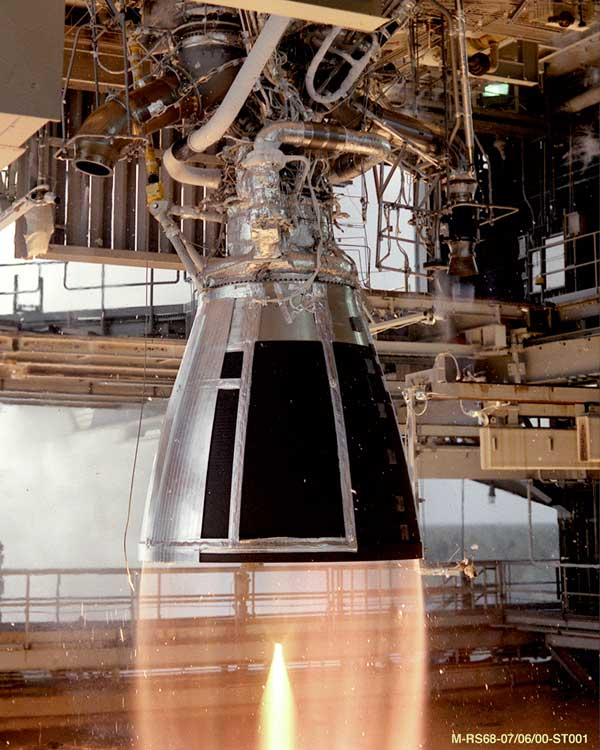
\includegraphics[height=\paperheight]{RS-68_rocket_engine_test.jpg}};
\fill[white,opacity=.91] (0,0) rectangle (595.276,89.5);
\fill[studiumInk,opacity=.96] (0,585.5) rectangle (595.276,841.89);
\node[anchor=west,text=studiumInk,font=\sffamily\bfseries\fontsize{18}{20}\selectfont,inner sep=0pt] at (51.223,38.5){STUDIUM};
\fill[studiumCyan] (51.223,61.5) rectangle (80.8,63.7);
\node[anchor=west,text=studiumInk,font=\sffamily\fontsize{9}{11}\selectfont,inner sep=0pt] at (89.49,65.5){BIBLIOTECA DE INGENIERÍA};
\node[anchor=west,text=studiumCyan,font=\sffamily\bfseries\fontsize{10}{12}\selectfont,inner sep=0pt] at (51.223,608){MANUAL UNIVERSITARIO};
\node[anchor=north west,text=white,text width=493pt,font=\rmfamily\bfseries\fontsize{33}{36}\selectfont,inner sep=0pt] at (51.223,636){#1};
\node[anchor=west,text=white!82!studiumInk,font=\sffamily\fontsize{11}{14}\selectfont,inner sep=0pt] at (51.223,732){#2};
\node[anchor=west,text=white,font=\sffamily\bfseries\fontsize{10}{12}\selectfont,inner sep=0pt] at (51.223,758){GRADO EN INGENIERÍA AEROESPACIAL};
\node[anchor=west,text=white!82!studiumInk,font=\sffamily\fontsize{10}{12}\selectfont,inner sep=0pt] at (51.223,773){Universidad de León};
\draw[white!75!studiumInk,line width=.4pt] (51.223,786) -- (544.05,786);
\node[anchor=west,text=white!82!studiumInk,font=\sffamily\fontsize{10}{12}\selectfont,inner sep=0pt] at (51.223,810){2026};
\node[anchor=east,text=white,font=\sffamily\bfseries\fontsize{10}{12}\selectfont,inner sep=0pt] at (544.05,810){I Edición};
\end{scope}\end{tikzpicture}\null\end{titlepage}\hypersetup{pageanchor=true}}

\hypersetup{pdftitle={MOTORES COHETE},pdfauthor={Daniel Miguel Tejedor}}
\renewcommand{\studiumvolumetype}{manual}
\begin{document}
\studiumcover{MOTORES COHETE}{Fundamentos, sistemas propulsivos y actuaciones espaciales}{MANUAL UNIVERSITARIO}
\frontmatter
\studiumreadingguide
\chapter*{Presentación y alcance}
\addcontentsline{toc}{chapter}{Presentación y alcance}
Este volumen pertenece al proyecto independiente de Motores Cohete, Universidad de León, curso 2026/2027. Es una elaboración original de apoyo al estudio, sin atribución de autoría ni aval a la Universidad. Los controles ejecutados y su alcance se detallan en los informes, junto con las comprobaciones pendientes.

La estructura académica conserva los seis bloques de la guía oficial. Los 28 capítulos, los problemas y los simulacros son decisiones editoriales. Los documentos proporcionados se abrieron y contrastaron; los manuscritos estudiantiles se usan para analizar competencias y posibles errores, sin copiar páginas, figuras ni enunciados extensos.

Los modelos se acompañan de hipótesis y límites. La reproducción aritmética, el álgebra simbólica, las dimensiones, la conservación y la validación experimental son niveles diferentes. Una solución de equilibrio o una curva ideal no se presenta como un ensayo real.

La procedencia técnica y los controles ejecutados se conservan en el repositorio del libro.

Se adopta $g_0=9.80665\,\mathrm{m/s^2}$ y unidades SI. Los decimales adicionales de algunas soluciones facilitan comprobar cálculos; no representan precisión experimental. Los niveles básico, intermedio, avanzado y de examen son orientativos.

El manual es autónomo: desarrolla teoría, derivaciones, figuras y 28 casos resueltos. Sus 112 ejercicios de estudio tienen respuestas en el apéndice H. Los cuadernos añaden datos y problemas originales para practicar y evaluar integración.
\tableofcontents
\listoffigures
\mainmatter
\part{Bloque 1. Introducción y fundamentos}
\chapter{Propulsión cohete: misiones y lenguaje físico}\label{ch:01}
\objetivos{Distinguir fuente de energía y masa de reacción; clasificar los sistemas propulsivos; relacionar los requisitos de una misión con empuje, impulso y potencia; separar dato, modelo y verificación.}
\section{Qué hace un sistema propulsivo}
Un motor cohete transfiere cantidad de movimiento a una masa que expulsa. El vehículo recibe la reacción correspondiente. La conservación se aplica al conjunto vehículo más materia expulsada; aplicada sólo a la parte que permanece a bordo requiere contabilizar el flujo de masa. Esta distinción explica por qué no es necesario empujar contra el aire y por qué un sistema puede funcionar en vacío. El entorno modifica presiones, intercambio térmico y fuerzas externas, pero no proporciona la reacción indispensable para la propulsión.

Conviene separar tres preguntas. La primera es qué sustancia abandona el vehículo: la masa de reacción. La segunda es de dónde procede la energía que permite acelerarla. La tercera es cómo se transforma esa energía en movimiento dirigido. En un motor químico las sustancias transportadas participan en reacciones que cambian su energía química. En un propulsor eléctrico, una fuente eléctrica aporta una parte esencial de la energía; el fluido puede calentarse, ionizarse o acelerarse mediante campos. La fuente eléctrica y el propulsante no son necesariamente el mismo subsistema.

La palabra \emph{propulsante} incluye la materia consumida por la propulsión. En un bipropulsante químico comprende combustible y oxidante; usar sólo el caudal de combustible en el denominador del impulso específico produciría una comparación falsa. Un monopropulsante no se define por almacenar combustible sin oxidante, sino por funcionar con una sustancia que puede liberar energía mediante un proceso adecuado sin un segundo propulsante separado. Un sólido puede contener componentes de distintas funciones distribuidos en una matriz; su clasificación no sustituye al análisis de su respuesta mecánica y térmica.

Las magnitudes de interés se definen antes de calcular. El empuje $F$ es una fuerza, en newtons. El impulso total es una integral temporal, en newton segundo. El caudal $\dot m$ es masa por tiempo. La velocidad efectiva $c=F/\dot m$ tiene dimensiones de velocidad aunque incluya un término de presión y no coincida con la velocidad física en la salida. El impulso específico $I_{sp}=c/g_0$ se expresa en segundos; $g_0=9.80665\,\mathrm{m\,s^{-2}}$ es una constante convencional, no la aceleración gravitatoria en la posición del vehículo.
\section{Clasificar para formular modelos}
Los motores químicos térmicos convierten energía interna y química en entalpía de los productos, y una tobera transforma parte de ella en energía cinética dirigida. La clasificación en sólidos, líquidos e híbridos informa sobre almacenamiento y mecanismos de suministro. No determina por sí sola el impulso específico, la estabilidad, el número de encendidos o el grado de regulación. Esas propiedades requieren examinar la arquitectura concreta y las condiciones de operación.

En un sólido, la superficie reactiva evoluciona al consumirse material. Su caudal no es una variable arbitraria: resulta del acoplamiento entre regresión, presión y descarga. En un líquido, las líneas de alimentación, la inyección, la combustión y la tobera forman una red acoplada. Las bombas aumentan presión a costa de potencia; el sistema que la proporciona participa en el balance completo. En un híbrido las fases de los propulsantes son distintas y la regresión puede estar asociada al flujo que recorre la superficie. No debe trasladarse automáticamente una ley empírica de un sólido a un híbrido.

La propulsión eléctrica comprende sistemas electrotérmicos, electrostáticos y electromagnéticos. Un Hall contiene campos magnéticos importantes para el transporte electrónico, pero la aceleración principal de los iones se asocia al campo eléctrico. Clasificarlo por la mera presencia de un imán ocultaría la física que se pretende estudiar. En todos los casos hay que cerrar un presupuesto de potencia, masa, impulso y tiempo de operación.

Las comparaciones requieren fronteras homogéneas. Una comparación de masas puede incluir sólo el propulsante, el sistema de alimentación, el motor seco o el subsistema completo con fuente de energía. Una comparación de rendimiento puede referirse a la energía del chorro, la conversión eléctrica o la utilidad para una maniobra. Ninguna de estas razones es una eficiencia universal del vehículo.
\section{Empuje, duración y utilidad de una misión}
La ecuación ideal del cohete relaciona una velocidad efectiva con una razón de masas. No dice cuánto tarda la maniobra. Si dos sistemas producen el mismo impulso total, no necesariamente llevan a cabo la misma trayectoria: durante tiempos distintos actúan fuerzas externas y cambian las condiciones orbitales. Tampoco el impulso total basta para comparar dos motores que aceleran vehículos con masas diferentes.

Para una descarga unidireccional ideal, sin presión adicional, se tiene
\begin{align}
 F&=\dot m v_e, & \dot E_j&=\frac12\dot m v_e^2,\\
 \frac{\dot E_j}{F}&=\frac{v_e}{2}, & F&=\frac{2\dot E_j}{v_e}.
\end{align}
La primera relación cuenta momento; la segunda cuenta energía cinética del chorro respecto al motor. A potencia de chorro fijada, aumentar la velocidad de escape reduce el empuje. No es una contradicción: se consume menos masa, pero cada kilogramo exige más energía. Esta relación será central en propulsión eléctrica. No se aplica sin modificación si se confunden potencia eléctrica de entrada y potencia dirigida del chorro.

En una misión espacial aparecen restricciones adicionales: tiempo disponible, orientación, masa de los depósitos, almacenamiento, potencia solar, disipación térmica y fiabilidad. Un sistema de alto $I_{sp}$ puede ahorrar propulsante y necesitar una fuente de potencia cuya masa elimine esa ventaja. Un motor de gran empuje puede reducir pérdidas gravitatorias y, a la vez, exigir estructura o alimentación más pesada. La decisión requiere un problema de sistema, no ordenar una tabla por un único número.
\section{De la historia a una forma de razonar}
Como hitos documentados, NASA sitúa el primer vuelo de un cohete de propulsante líquido de Robert Goddard el 16 de marzo de 1926, en Auburn, Massachusetts. El lanzamiento de Sputnik el 4 de octubre de 1957 abrió la etapa de satélites artificiales en órbita. Son hitos de demostración y de misión distintos: hacer funcionar una arquitectura propulsiva y alcanzar una condición orbital no exigen el mismo conjunto de prestaciones.\cite{NASA-GODDARD,NASA-SPUTNIK}

La evolución posterior puede entenderse mediante compromisos de sistema. Un lanzador necesita mucho empuje durante una fase breve; una sonda con energía eléctrica puede acumular un gran cambio de velocidad a lo largo de intervalos prolongados. En la historia de la propulsión eléctrica descrita por Goebel y Katz, el desarrollo de fuentes de plasma, aceleración y sistemas de potencia permitió pasar de demostraciones a aplicaciones de mantenimiento orbital y misiones científicas. No es una sustitución universal de la propulsión química: amplía el conjunto de soluciones disponibles para objetivos distintos.

La historia de la propulsión no consiste sólo en una sucesión de récords. El reconocimiento de la masa variable permitió separar la necesidad de transportar masa de reacción de la necesidad de una atmósfera. El desarrollo de toberas supersónicas hizo posible convertir una mayor fracción de entalpía en velocidad dirigida. Las arquitecturas líquidas añadieron capacidad de suministro y control; los sólidos aportaron otras formas de almacenamiento e integración; la propulsión eléctrica amplió el compromiso entre consumo y duración.

Estos avances no invalidaron las conservaciones. Cambiaron los mecanismos con los que se satisfacen y los límites de los modelos simplificados. Un mismo balance de momento permite estudiar una tobera química o un haz de iones, pero las ecuaciones constitutivas que suministran el caudal, la energía y las fuerzas internas son diferentes. Esa continuidad conceptual es más útil que memorizar una fórmula distinta para cada tecnología.

En este manual los seis bloques proceden de la documentación docente ULE; los 28 capítulos son una división editorial. La guía establece 6 ECTS y 150 horas de trabajo, con un 75\,\% de prueba escrita y un 25\,\% de trabajo y defensa. Los tiempos y puntuaciones de los simulacros son propuestas de estudio. La oferta de TFG y TFM acompaña a los materiales, pero no se utiliza como programa de la asignatura.\cite{GUIA2026,ULE-PRES}
\section{Problema resuelto: dos sistemas con distinta velocidad efectiva}
\begin{studiumworked}{M01. Cantidad de movimiento y presupuesto de potencia}
\textbf{Enunciado y datos.} Dos modelos ideales entregan la misma potencia al chorro, $\dot E_j=600\,\mathrm W$. Sus velocidades son $v_{e,A}=3000\,\mathrm{m/s}$ y $v_{e,B}=18000\,\mathrm{m/s}$. Determine empuje, caudal e impulso en un intervalo de $120\,\mathrm s$.

\textbf{Incógnitas e hipótesis.} $F$, $\dot m$ e $I$. Régimen constante, chorro axial monocinético, entorno sin término de presión y potencia ya referida al chorro. No se prescribe una tecnología física ni una eficiencia eléctrica.

\textbf{Modelo y despeje.} Conservar momento y energía da
\[F=2\dot E_j/v_e,\qquad \dot m=2\dot E_j/v_e^2,\qquad I=F\Delta t.\]
\textbf{Sustitución y resultados.} Para A: $F_A=1200/3000=0.400\,\mathrm N$, $\dot m_A=1.33333\times10^{-4}\,\mathrm{kg/s}$ e $I_A=48.0\,\mathrm{N\,s}$. Para B: $F_B=0.0666667\,\mathrm N$, $\dot m_B=3.70370\times10^{-6}\,\mathrm{kg/s}$ e $I_B=8.00\,\mathrm{N\,s}$.

\textbf{Interpretación.} Multiplicar por seis la velocidad divide el empuje por seis y el caudal por 36 a potencia fija. La masa ahorrada no se convierte automáticamente en una maniobra más rápida.

\textbf{Comprobación.} En ambos casos $Fv_e/2=600\,\mathrm W$ y $I=\Delta m\,v_e$. Las dimensiones de $2\dot E_j/v_e$ son newtons. \textbf{Límites.} Se excluyen divergencia, distribuciones de velocidad, pérdidas, masa de la fuente y variación de masa del vehículo.
\textbf{Operaciones para comparar ambos casos.}
\begin{enumerate}

\item Despejar empuje de potencia cinética: F=2P/v.

\[\fitmath{\mathrm{FA}=\frac{2\cdot 600}{3000}\approx 0.4\,\mathrm{N}}\]

\item Del balance de energía, caudal es 2P/v al cuadrado.

\[\fitmath{\mathrm{mA}=\frac{2\cdot 600}{{3000}^{2}}\approx 0.0001333333\,\mathrm{kg/s}}\]

\item Integrar empuje constante durante el intervalo.

\[\fitmath{\mathrm{IA}=\mathrm{FA}\cdot 120}\]

\[\fitmath{\mathrm{IA}=(0.4)\cdot 120\approx 48\,\mathrm{N\,s}}\]

\item Repetir el balance de momento y energía con la segunda velocidad.

\[\fitmath{\mathrm{FB}=\frac{2\cdot 600}{18000}\approx 0.06666667\,\mathrm{N}}\]

\item Calcular el segundo caudal.

\[\fitmath{\mathrm{mB}=\frac{2\cdot 600}{{18000}^{2}}\approx 3.703704\times10^{-6}\,\mathrm{kg/s}}\]

\item Impulso del segundo caso.

\[\fitmath{\mathrm{IB}=\mathrm{FB}\cdot 120}\]

\[\fitmath{\mathrm{IB}=(0.06666666667)\cdot 120\approx 8\,\mathrm{N\,s}}\]

\end{enumerate}

\end{studiumworked}
\figura{c01}{A potencia de chorro fija, aumentar la rapidez reduce el empuje. Modelo axial monocinético, sin término de presión.}
\section{Ejercicios propuestos}
\begin{enumerate}
\item Explique por qué un cohete funciona en vacío y por qué no puede prescindir de masa de reacción en el modelo descrito.
\item Un empuje constante de $0.12\,\mathrm N$ actúa durante $250\,\mathrm s$. Halle el impulso y distíngalo de un incremento de velocidad.
\item A potencia de chorro constante, duplique $v_e$. Prediga las razones de empuje, caudal e impulso específico antes de calcular.
\item Compare dos presupuestos de masa: uno que incluye sólo propulsante y otro que incluye fuente eléctrica. ¿Qué conclusión puede cambiar?
\end{enumerate}
\resumen{El sistema intercambia momento con materia expulsada. Empuje, impulso total e impulso específico no son intercambiables. Una elevada velocidad efectiva ahorra propulsante en ciertos modelos, pero exige energía y puede reducir el empuje. La elección depende de la misión y de una frontera de sistema explícita.}


\studiumchaptercheck

\chapter{Balances integrales y ecuación de empuje}\label{ch:02}
\objetivos{Formular balances con un volumen de control; obtener el término de presión sin duplicarlo; pasar de una distribución de salida a una velocidad efectiva; integrar el impulso cuando varía el caudal.}
\section{Sistema material y volumen de control}
Un sistema material contiene siempre las mismas partículas. Para él, la suma de fuerzas externas es la derivada de su cantidad de movimiento. Un motor, considerado como región geométrica, recibe y expulsa materia: no es ese sistema cerrado. El teorema de transporte de Reynolds relaciona ambos puntos de vista. Para una propiedad extensiva con valor por unidad de masa $b$, un volumen que se mueve con velocidad superficial $\mathbf v_s$ satisface
\begin{equation}
\frac{d B_{\rm sist}}{dt}=\frac{\partial}{\partial t}\int_{VC}\rho b\,dV+
\int_{SC}\rho b(\mathbf v-\mathbf v_s)\cdot\mathbf n\,dA.
\end{equation}
La normal es exterior. El producto escalar distingue automáticamente entradas y salidas. Omitir la velocidad relativa de cruce en un volumen móvil equivale a contar incorrectamente la masa que lo atraviesa.

Para masa, $b=1$ y $dB_{\rm sist}/dt=0$. En un volumen fijo respecto al motor y con velocidades relativas $\mathbf u$,
\begin{equation}
\frac{d}{dt}\int_{VC}\rho\,dV+\int_{SC}\rho\mathbf u\cdot\mathbf n\,dA=0.
\end{equation}
La hipótesis estacionaria elimina el almacenamiento, no las entradas ni las salidas. Para un motor que recibe dos corrientes y expulsa una, $\dot m_e=\dot m_f+\dot m_o$ sólo si no hay acumulación ni otras descargas. En un ciclo con gases auxiliares vertidos al exterior, esos gases también consumen propulsante y aportan o sustraen momento según su dirección.
\section{Balance de momento y fuerza propulsiva}
Tomemos un eje positivo hacia delante del vehículo. La velocidad de salida relativa tiene componente axial $-v_e$. El motor ejerce sobre el fluido una fuerza hacia atrás; el fluido ejerce sobre el motor la opuesta. Para derivar el empuje del sistema completo resulta cómodo incluir a bordo los depósitos, de modo que no aparezca una corriente externa de admisión. El caudal de escape atraviesa la sección posterior y su flujo de momento tiene que contabilizarse con el convenio de signos elegido.

La presión actúa sobre toda la superficie del vehículo, no únicamente sobre la salida imaginaria del volumen de control. Una presión ambiente espacialmente uniforme produce fuerza neta nula sobre una superficie cerrada. Al cerrar geométricamente la abertura de salida y restar esa contribución uniforme, aparece la diferencia $p_e-p_a$. Con régimen estacionario, salida uniforme, axial y plana, y despreciando otras fuerzas sobre el motor,
\begin{equation}\label{eq:thrust}
 F=\dot m v_e+(p_e-p_a)A_e.
\end{equation}
No se ha supuesto $p_e=p_a$. El término puede ser positivo, cero o negativo. Si se omite sin verificar adaptación, no se obtiene una aproximación controlada sino otro modelo. El hecho de que el término de presión sea negativo no demuestra que el empuje total lo sea; tampoco garantiza que una solución supersónica adherida exista a esa contrapresión.

La forma integral adecuada para una salida no uniforme es
\begin{equation}
 F_x=-\int_{A_e}\rho u_x(\mathbf u\cdot\mathbf n)\,dA-
 \int_{A_e}(p-p_a)\,n_x\,dA,
\end{equation}
con normal exterior y componentes de velocidad referidas al eje positivo hacia delante. Los signos menos convierten la fuerza sobre el fluido en su reacción sobre el motor. Si se usan magnitudes positivas de descarga hacia atrás, el primer término se escribe como flujo axial positivo de momento. Es imprescindible indicar qué magnitud representa $u_x$ antes de copiar la forma vectorial. Una velocidad media aritmética no reproduce necesariamente la integral de $\rho u^2$: la media relevante para el momento está ponderada por flujo másico.\cite{MIT02,NASA-THRUST}
\section{Velocidad física, efectiva y característica}
Dividir \eqref{eq:thrust} por el caudal total da
\begin{equation}\label{eq:ceff}
 c\equiv\frac{F}{\dot m}=v_e+\frac{(p_e-p_a)A_e}{\dot m}.
\end{equation}
Cada sumando tiene unidades de $\mathrm{m/s}$. La velocidad efectiva es una forma de expresar momento por masa consumida; no es la velocidad que mediría una sonda en el plano de salida cuando existe empuje de presión. Esa distinción permite describir con un solo parámetro la dinámica ideal del vehículo, siempre que el balance cuente una sola vez todas las contribuciones.

La velocidad característica se define de otra manera:
\begin{equation}
 c^*\equiv\frac{p_cA_t}{\dot m},\qquad C_F\equiv\frac{F}{p_cA_t},\qquad c=C_Fc^*.
\end{equation}
La identidad final procede de las definiciones; no necesita hipótesis isentrópicas. Sin embargo, predecir $c^*$ a partir de temperatura, composición y $\gamma$ sí exige un modelo de descarga. Medir $p_c$, $A_t$ y $\dot m$ produce un valor experimental de $c^*$; introducir una fórmula de gas perfecto produce un valor de modelo. No se deben intercambiar sus significados.

La página NASA sobre impulso específico consultada presenta en una de sus expresiones una agrupación que suma velocidad y fuerza antes de dividir por caudal. Se conserva la discrepancia en la auditoría. La ecuación dimensionalmente consistente es \eqref{eq:ceff}; la institución que publica una página no elimina la necesidad de revisar su álgebra.\cite{NASA-ISP}
\section{Impulso total e impulso específico variable}
El impulso total sobre un intervalo es
\begin{equation}
 I=\int_{t_0}^{t_f}F(t)\,dt.
\end{equation}
Si $F$ cambia, sustituir la integral por el valor máximo multiplicado por duración sobreestima el impulso. La aproximación por un promedio temporal es exacta sólo cuando ese promedio es el de la señal en el intervalo considerado. El impulso específico instantáneo y el del intervalo son, respectivamente,
\begin{align}
 I_{sp}(t)&=\frac{F(t)}{g_0\dot m(t)},\\
 \overline I_{sp}&=\frac{I}{g_0\Delta m_p}
 =\frac{\int I_{sp}(t)\dot m(t)\,dt}{\int\dot m(t)\,dt}.
\end{align}
El segundo es un promedio ponderado por masa consumida. Promediar aritméticamente dos impulsos específicos sólo funciona si las masas consumidas en las dos partes son iguales. En una comparación con distinta presión ambiente, el término de presión modifica $F$ y, por tanto, el impulso específico, aun con el mismo caudal y estado de cámara.

El valor de $g_0$ no cambia en una misión lunar. Lo que cambia con el lugar es la fuerza gravitatoria externa, que entra en las ecuaciones del vehículo. Si se sustituye la gravedad local en la definición de $I_{sp}$, se fabricaría una mejora de prestaciones sin cambiar el motor.
\section{Energía y momento angular}
Para una corriente estacionaria, el balance de energía por unidad de tiempo incluye entalpía, energía cinética y potencial. El trabajo de flujo ya está contenido en $h=e+p/\rho$:
\begin{equation}
 \dot Q-\dot W_s=\sum_{\rm sal}\dot m\left(h+\frac{u^2}{2}+gz\right)
 -\sum_{\rm ent}\dot m\left(h+\frac{u^2}{2}+gz\right).
\end{equation}
En una tobera adiabática sin trabajo de eje y con cambio de altura despreciable, $h+u^2/2$ se conserva. No se sigue que la entropía se conserve: un choque puede mantener la entalpía de remanso y aumentar la entropía. Una cámara reactiva requiere entalpías que incluyan referencias de formación; sumarle después otra vez el calor químico liberado contaría dos veces la misma energía.

En una turbomáquina también interesa el momento angular respecto al eje. La diferencia de flujo de $r u_\theta$ proporciona el par. Al multiplicarlo por velocidad angular se obtiene potencia de eje. Este balance conducirá a la ecuación de Euler, pero la energía transferida no determina por sí sola la altura útil: las pérdidas internas requieren un rendimiento y condiciones de entrada.
\section{Problema resuelto: separación del empuje de presión}
\begin{studiumworked}{M02. Un mismo escape en dos ambientes}
\textbf{Datos y pregunta.} Un modelo estacionario tiene $\dot m=2.40\,\mathrm{kg/s}$, $v_e=2500\,\mathrm{m/s}$, $p_e=45.0\,\mathrm{kPa}$ y $A_e=0.0120\,\mathrm{m^2}$. Calcule $F$, $c$ e $I_{sp}$ para $p_a=90.0\,\mathrm{kPa}$ y para vacío.

\textbf{Hipótesis y modelo.} Salida uniforme axial y estado interno invariable entre los dos cálculos; la hipótesis de adherencia se declara, no se demuestra aquí. Se utiliza \eqref{eq:thrust}, no una ecuación de motor adaptado.

\textbf{Despeje y sustitución.} $F=2.40(2500)+(45000-p_a)(0.0120)$. El término cinético vale $6000\,\mathrm N$. En el primer ambiente el término de presión es $-540\,\mathrm N$; en vacío es $+540\,\mathrm N$.

\textbf{Resultados.} $F_{90}=5460\,\mathrm N$, $c_{90}=2275\,\mathrm{m/s}$ e $I_{sp,90}=231.985\,\mathrm s$; $F_v=6540\,\mathrm N$, $c_v=2725\,\mathrm{m/s}$ e $I_{sp,v}=277.873\,\mathrm s$.

\textbf{Interpretación y comprobación.} La diferencia $F_v-F_{90}=1080\,\mathrm N$ coincide con $p_aA_e$. El valor de $v_e$ no cambió, pero sí el de $c$. Multiplicar cada $I_{sp}$ por $g_0$ recupera su velocidad efectiva. \textbf{Límites.} No se ha calculado separación ni respuesta del caudal a contrapresión; por ello no se afirma que el primer estado corresponda a una tobera real estable.
\textbf{Operaciones para comparar ambos casos.}
\begin{enumerate}

\item Contribución cinética del caudal.

\[\fitmath{\mathrm{Fk}=2.4\cdot 2500\approx 6000\,\mathrm{N}}\]

\item Presión residual en el primer ambiente.

\[\fitmath{\mathrm{Fp}_{90}=\left(45000-90000\right)\cdot 0.012\approx -540\,\mathrm{N}}\]

\item Sumar contribuciones del mismo balance.

\[\fitmath{F_{90}=\mathrm{Fk}+\mathrm{Fp}_{90}}\]

\[\fitmath{F_{90}=(6000)+(-540)\approx 5460\,\mathrm{N}}\]

\item Velocidad efectiva incluye presión.

\[\fitmath{c_{90}=\frac{F_{90}}{2.4}}\]

\[\fitmath{c_{90}=\frac{(5460)}{2.4}\approx 2275\,\mathrm{m/s}}\]

\item Pasar a impulso específico convencional.

\[\fitmath{\mathrm{Isp}_{90}=\frac{c_{90}}{9.80665}}\]

\[\fitmath{\mathrm{Isp}_{90}=\frac{(2275)}{9.80665}\approx 231.9854\,\mathrm{s}}\]

\item En vacío se resta presión ambiente cero.

\[\fitmath{\mathrm{Fv}=\mathrm{Fk}+45000\cdot 0.012}\]

\[\fitmath{\mathrm{Fv}=(6000)+45000\cdot 0.012\approx 6540\,\mathrm{N}}\]

\item Velocidad efectiva de vacío.

\[\fitmath{\mathrm{cv}=\frac{\mathrm{Fv}}{2.4}}\]

\[\fitmath{\mathrm{cv}=\frac{(6540)}{2.4}\approx 2725\,\mathrm{m/s}}\]

\item Impulso específico de vacío.

\[\fitmath{\mathrm{Ispv}=\frac{\mathrm{cv}}{9.80665}}\]

\[\fitmath{\mathrm{Ispv}=\frac{(2725)}{9.80665}\approx 277.8727\,\mathrm{s}}\]

\end{enumerate}

\end{studiumworked}
\figura{c02}{El escape cruza hacia atrás y la reacción propulsiva apunta hacia delante. El cierre de presión utiliza la diferencia entre salida y ambiente.}
\section{Ejercicios propuestos}
\begin{enumerate}
\item Deduzca las dimensiones de $c^*$, $C_F$, $I$ e $I_{sp}$ sin utilizar sus nombres.
\item Dos fases consumen 2 y 5 kg con impulsos específicos 240 y 300 s. Determine el valor del intervalo y explique el promedio empleado.
\item Una descarga auxiliar consume el 4\,\% del propulsante total. ¿Por qué no basta con usar el caudal de la cámara principal en el denominador de prestaciones del sistema?
\item Demuestre que omitir el término de presión y sumarlo después en $c$ duplicaría su contribución si se emplea ya $F=\dot m c$.
\end{enumerate}
\resumen{El balance de momento se cierra con presiones relativas al ambiente y flujos de masa definidos respecto al volumen de control. $c$, $v_e$ y $c^*$ son magnitudes diferentes. El impulso específico global es un promedio por masa consumida, y $g_0$ es convencional. El balance energético no permite inferir isentropía.}


\studiumchaptercheck

\chapter{Termodinámica de los gases propulsivos}\label{ch:03}
\objetivos{Distinguir gas ideal, composición congelada y gas caloríficamente perfecto; obtener las relaciones de remanso; incorporar la entropía y las referencias de energía química.}
\section{Variables de estado y escalas de masa}
Para un gas ideal simple, $p=\rho R T$. La constante específica pertenece a la composición: $R=R_u/\mathcal M$, donde $R_u=8314.462618\,\mathrm{J/(kmol\,K)}$ si $\mathcal M$ se expresa en $\mathrm{kg/kmol}$. También puede emplearse $R_u=8.314462618\,\mathrm{J/(mol\,K)}$ y masa molar en $\mathrm{kg/mol}$. Mezclar ambas convenciones introduce un factor mil. La unidad no se decide por el aspecto numérico de la masa molar.

Una mezcla ideal tiene fracciones molares $x_i=n_i/\sum n_j$ y másicas $Y_i=m_i/\sum m_j$. Con masas molares $\mathcal M_i$,
\begin{align}
\mathcal M&=\sum_i x_i\mathcal M_i,
&Y_i&=\frac{x_i\mathcal M_i}{\mathcal M},\\
\frac{1}{\mathcal M}&=\sum_i\frac{Y_i}{\mathcal M_i},
&R&=R_u\sum_i\frac{Y_i}{\mathcal M_i}.
\end{align}
Promediar directamente las masas molares con fracciones másicas no da la masa molar de mezcla. La ecuación de estado ideal tampoco obliga a que las fracciones sean constantes: esa es una hipótesis independiente sobre química o transporte de especies.
\section{Energía interna, entalpía y calores específicos}
La entalpía $h=e+p/\rho$ incorpora el trabajo de desplazar fluido a través de la frontera. Para composición fija y gas ideal, $e=e(T)$ y $h=h(T)$. Las derivadas $c_v=de/dT$ y $c_p=dh/dT$ satisfacen $c_p-c_v=R$. Sólo si son constantes se obtiene
\begin{equation}
 h(T)-h(T_r)=c_p(T-T_r),\qquad
 c_p=\frac{\gamma R}{\gamma-1},\qquad \gamma=\frac{c_p}{c_v}.
\end{equation}
Un gas térmicamente perfecto obedece la ecuación ideal con composición fija, pero puede tener $c_p(T)$. En tal caso se integra $h(T)-h(T_r)=\int_{T_r}^{T}c_p(\vartheta)\,d\vartheta$. Tratar ese gas mediante una única potencia de temperatura necesita una aproximación adicional, cuyo intervalo debe declararse.

En una mezcla reactiva, el cambio de $h$ incluye cambios de especies. Se escribe
\begin{equation}
 h(T,\mathbf Y)=\sum_iY_i\left[h_{f,i}^{\circ}+\int_{T_r}^{T}c_{p,i}(\vartheta)\,d\vartheta\right].
\end{equation}
Las entalpías de formación y las integrales deben compartir referencias. Los ceros individuales de entalpía son convencionales, pero no se pueden modificar de forma independiente entre reactantes y productos en un balance de reacción. Para un reactor adiabático, con energía cinética despreciable y sin trabajo de eje, la entalpía total de salida iguala la de entrada. La liberación química ya está representada mediante los términos de formación.
\section{Entropía y relaciones isentrópicas}
La identidad de Gibbs para una sustancia simple de composición fija es $T\,ds=dh-dp/\rho$. Con la ecuación ideal,
\begin{equation}\label{eq:gibbs}
 ds=c_p(T)\frac{dT}{T}-R\frac{dp}{p}.
\end{equation}
Si $c_p$ es constante y $ds=0$, integrar entre dos estados da
\begin{align}
 c_p\ln\frac{T_2}{T_1}&=R\ln\frac{p_2}{p_1},\\
 \frac{T_2}{T_1}&=\left(\frac{p_2}{p_1}\right)^{(\gamma-1)/\gamma}, &
 \frac{p_2}{p_1}&=\left(\frac{\rho_2}{\rho_1}\right)^\gamma.
\end{align}
Estas expresiones comparan estados conectados isentrópicamente del mismo gas caloríficamente perfecto. No son leyes generales de toda expansión. Con un choque o fricción adiabática puede conservarse energía total y aumentar la entropía. Con composición cambiante, la relación de Gibbs incorpora potenciales químicos y no se reduce sin más a \eqref{eq:gibbs} con un $R$ escogido a posteriori.

El balance de entropía de un volumen de control incluye transporte con las corrientes, transferencia de calor a temperatura de frontera y generación interna $\dot S_{gen}\geq0$. La desigualdad es una condición física, no una corrección algebraica opcional. Un rendimiento no puede utilizarse para ocultar una reducción de entropía incompatible con un proceso adiabático irreversible.
\section{Velocidad del sonido y magnitudes de remanso}
La velocidad de una perturbación isentrópica infinitesimal es
\begin{equation}
 a^2=\left(\frac{\partial p}{\partial\rho}\right)_s.
\end{equation}
Usando $p/\rho^\gamma=$ constante se obtiene $a^2=\gamma p/\rho=\gamma RT$. Esta deducción presupone una respuesta calorífica y composicional coherente con la perturbación. En un gas reactivo, la velocidad acústica puede corresponder a una respuesta congelada o de equilibrio según las escalas temporales; no basta con introducir el cociente de dos calores específicos impresos en una tabla.

Se define $h_0=h+u^2/2$ para detener idealmente la corriente sin cambio de altura. Una detención adiabática sin trabajo conserva esa magnitud. Para el modelo de $c_p$ constante,
\begin{align}
 c_pT_0&=c_pT+\frac{u^2}{2},\\
 \frac{T_0}{T}&=1+\frac{u^2}{2c_pT}
 =1+\frac{\gamma-1}{2}M^2,\qquad M=\frac{u}{\sqrt{\gamma RT}}.
\end{align}
Si la detención de referencia es además isentrópica,
\begin{equation}\label{eq:stagnation}
 \frac{p_0}{p}=\left(1+\frac{\gamma-1}{2}M^2\right)^{\gamma/(\gamma-1)},\qquad
 \frac{\rho_0}{\rho}=\left(1+\frac{\gamma-1}{2}M^2\right)^{1/(\gamma-1)}.
\end{equation}
La presión de remanso es una propiedad de referencia asociada al estado local y al proceso isentrópico de detención. A través de un choque adiabático $T_0$ permanece constante en el modelo simple, mientras que $p_0$ disminuye. Esta diferencia es una medida útil de irreversibilidad.

La presión de cámara $p_c$ suele aproximarse a $p_0$ porque la velocidad en la cámara es pequeña. Si no lo es, la aproximación debe corregirse con el Mach de cámara. Una medida de presión estática en una cámara de contracción finita no debe interpretarse automáticamente como presión total.
\section{Pérdidas, trabajo útil y comparación de procesos}
El rendimiento de tobera puede definirse como la energía cinética real obtenida dividida por el descenso entálpico isentrópico disponible entre referencias especificadas. Para velocidad de entrada despreciable,
\[\eta_n=\frac{v_{e,r}^2}{v_{e,s}^2},\qquad v_{e,r}=\sqrt{\eta_n}\,v_{e,s}.\]
Esto no implica $F_r=\eta_n F_s$ ni $c_r=\eta_n c_s$: el empuje incluye presión y la velocidad recibe la raíz del rendimiento. Además, si la pérdida cambia caudal o estado de salida, es necesario recalcular el balance completo.

En la aproximación caloríficamente perfecta, la caída isentrópica de entalpía entre cámara y salida es
\begin{equation}
 \frac{v_e^2}{2}=\frac{\gamma}{\gamma-1}RT_c
 \left[1-\left(\frac{p_e}{p_c}\right)^{(\gamma-1)/\gamma}\right].
\end{equation}
El límite $p_e/p_c\to0$ produce una velocidad finita porque la entalpía inicial es finita. Si el modelo exige temperatura final tendente a cero, su realismo termodinámico se deteriora antes de alcanzar ese límite matemático. La existencia del límite no valida la extrapolación de $c_p$ constante hasta cero kelvin.\cite{MIT03,MIT12,CEA-RP1}
\section{Aplicación y estudio activo}
El caso M03 de este capítulo calcula estados estáticos y de remanso y contrasta las dos rutas energéticas. Antes de sustituir números debe anotarse si $T_c$ y $p_c$ representan magnitudes totales. La hoja de fórmulas conserva estas hipótesis para evitar que una igualdad local se convierta en una receta universal.
\figura{c03}{Relaciones de remanso para un gas caloríficamente perfecto. Las curvas suponen composición fija e isentropía.}
\section{Caso desarrollado}
\begin{studiumworked}{M03. Dos rutas para la velocidad de una expansión · Intermedio}
\textbf{Enunciado.} Un gas académico de $\gamma=1.3$ y masa molar $23.3\,\mathrm{kg/kmol}$ tiene $T_0=2430$ K y $p_0=2.50$ MPa. Una sección isentrópica alcanza $M=2.075$. Halle $R,c_p,T,p,u$ y verifique energía.

\textbf{Datos.} Exponente constante: $1.3$; Masa molar: $23.3\,\mathrm{kg/kmol}$; Temperatura total: $2430\,\mathrm{K}$; Presión total: $2.500000\times10^{6}\,\mathrm{Pa}$; Mach: $2.075$.

\textbf{Incógnitas.} Propiedades específicas y estado estático.

\textbf{Hipótesis.} Gas caloríficamente perfecto de composición fija. Expansión adiabática reversible, sin trabajo ni altura.

\textbf{Modelo físico.} Energía y relaciones de remanso.
\[R=R_u/\mathcal M,\quad c_p=\gamma R/(\gamma-1)\]
\[T=T_0/[1+(\gamma-1)M^2/2]\]
\[p=p_0(T/T_0)^{\gamma/(\gamma-1)}\]
\[u=M\sqrt{\gamma RT}=\sqrt{2c_p(T_0-T)}\]
\textbf{Desarrollo.}
\begin{enumerate}
\item Se usa $R_u=8314.462618$ J/(kmol K), coherente con kg/kmol. Así $R=356.8439$ J/(kg K) y $c_p=1546.324$ J/(kg K).
\item El factor de remanso es $1.645844$. Dividir $T_0$ da $1476.446\,\mathrm{K}$; la potencia isentrópica da $288.5732\,\mathrm{kPa}$.
\item Con la temperatura estática, la ruta acústica da $1717.267\,\mathrm{m/s}$. La ruta energética usa el descenso $c_p(T_0-T)$ y produce el mismo valor. Usar $T_0$ dentro del sonido de la sección daría otra rapidez incompatible.
\end{enumerate}
\textbf{Operaciones para contrastar el cálculo.}
\begin{enumerate}

\item Magnitud 1.

\[\fitmath{y_{1}=\frac{8314.462618}{23.3}\approx 356.8439\,\mathrm{J/(kg\,K)}}\]

\item Magnitud 2.

\[\fitmath{y_{2}=2.075\cdot \sqrt{1.3\cdot 356.8438892\cdot 1476.446352}\approx 1717.267\,\mathrm{m/s}}\]

\item Magnitud 3.

\[\fitmath{y_{3}=1546.32352\cdot 1476.446352+\frac{{1717.266685}^{2}}{2}\approx 3757566\,\mathrm{J/kg}}\]

\end{enumerate}

\textbf{Resultados.} $T=1476.446$ K; $p=2.885732\times10^{5}$ Pa; $u=1717.267$ m/s.

\textbf{Interpretación.} El gas acelera y enfría, pero su temperatura total permanece fija. La presión total se mantiene sólo porque se ha supuesto isentropía.

\textbf{Comprobación.} $c_pT+u^2/2=c_pT_0=3.757566\times10^{6}$ J/kg. La entropía calculada mediante $c_p\ln(T/T_0)-R\ln(p/p_0)$ es cero dentro de redondeo.

\textbf{Límites.} No se modela química ni variación calorífica; gamma es un dato académico, no una propiedad universal de productos reales.
\end{studiumworked}

\section{Ejercicios propuestos}
\begin{enumerate}
\item Con $\mathcal M=24\,\mathrm{kg/kmol}$, determine $R$ y repita usando kg/mol. Los resultados deben coincidir.
\item Demuestre que al hacer $M\to0$, las magnitudes de remanso tienden a las estáticas.
\item Obtenga $ds$ entre dos estados y explique por qué no basta con comprobar que la temperatura disminuye para afirmar que una expansión es isentrópica.
\item ¿Puede mantenerse $T_0$ y disminuir $p_0$? Dé un mecanismo físico y la ecuación que detecta la irreversibilidad.
\end{enumerate}
\resumen{Gas ideal y gas caloríficamente perfecto son hipótesis diferentes. Las relaciones isentrópicas de potencias exigen composición y calores específicos constantes. La energía total puede conservarse con generación de entropía. Las referencias de formación son parte del balance reactivo, y las magnitudes de cámara no son siempre de remanso.}

\chapter{Parámetros característicos, pérdidas e incertidumbre}\label{ch:04}
\objetivos{Obtener las identidades entre prestaciones; definir rendimientos con fronteras coherentes; propagar incertidumbres; reconocer cuándo una comparación cambia de modelo.}
\section{Una jerarquía de definiciones}
Las definiciones proporcionan relaciones que no dependen de una tobera ideal:
\begin{align}
 c&=F/\dot m,& I_{sp}&=F/(\dot m g_0),\\
 c^*&=p_cA_t/\dot m,& C_F&=F/(p_cA_t),\\
 c&=C_Fc^*,& I_{sp}&=C_Fc^*/g_0.
\end{align}
De ellas no se deduce que $c^*$ sea constante, que $C_F$ sólo dependa de geometría ni que las prestaciones sean iguales en cualquier ambiente. Las predicciones requieren cerrar los estados y las condiciones de contorno. Por ejemplo, un cambio de garganta puede alterar el equilibrio de cámara de un sólido; su efecto no equivale al de cambiar un área en una cámara regulada a presión fija.

Cuando el sistema tiene más de una descarga, $F$ debe incluir sus contribuciones axiales y $\dot m$ todas las masas consumidas. De otro modo el impulso específico presentado sería el de una parte favorable del sistema y no el del conjunto. También conviene indicar si la presión usada en $c^*$ es estática medida o total estimada.
\section{Similitud y grupos adimensionales}
Para una tobera de gas caloríficamente perfecto, los grupos $A_e/A_t$, $p_a/p_c$ y $\gamma$ permiten describir el coeficiente de empuje ideal cuando se especifica el régimen. La temperatura y la constante específica establecen una escala de velocidad $\sqrt{RT_c}$. La escala de fuerza es $p_cA_t$ y la de caudal es $p_cA_t/\sqrt{RT_c}$.

Esas escalas explican por qué dos modelos geométricamente semejantes pueden tener el mismo $C_F$ y distinto empuje. No prueban semejanza de un motor real. La viscosidad introduce Reynolds; la transferencia térmica introduce Prandtl y razones de temperatura; la relajación química introduce tiempos característicos; la presencia de partículas añade tamaño, fracción de masa e inercia de fase. Dos sistemas con iguales $\gamma$ y relación de áreas pueden diferir en todos esos efectos.

El análisis dimensional es especialmente útil para descartar una expresión. No puede escoger entre dos expresiones dimensionalmente correctas con coeficientes distintos. Una fórmula que omite una pérdida puede conservar perfectamente sus unidades. Por ello la consistencia dimensional se registra separada de la fundamentación física y de la comprobación algebraica.
\section{Qué significa un rendimiento}
Sea $c^*_{id}$ un valor ideal calculado para reactantes, estados y modelo químico declarados. Una razón operacional $\eta_{c^*}=c^*_{med}/c^*_{id}$ resume discrepancias de cámara, pero no es una medida aislada de eficiencia de reacción si también hay errores de caudal, presión, área efectiva o composición. Es necesario distinguir la razón definida del mecanismo al que se atribuye.

Análogamente, $\eta_{C_F}=C_{F,r}/C_{F,id}$ puede representar una degradación respecto de un modelo de tobera. Si ambos cocientes emplean exactamente las mismas referencias,
\[\frac{I_{sp,r}}{I_{sp,id}}=\eta_{c^*}\eta_{C_F}.\]
No se puede multiplicar ese producto por otro rendimiento de velocidad ya incluido en $\eta_{C_F}$ sin contar dos veces una pérdida. Tampoco se garantiza que cualquier razón experimental se encuentre entre cero y uno cuando su referencia ideal fue elegida con hipótesis equivocadas. Un valor mayor que uno exige revisar referencias, incertidumbres y modelos; no se interpreta de inmediato como violación de la energía.

La eficiencia energética de un sistema eléctrico se define respecto de potencia eléctrica, mientras que $I_{sp}$ mide impulso por peso convencional de propulsante. Llamar al impulso específico ``rendimiento'' en una conversación abreviada no permite tratarlo como una fracción adimensional. Una cifra de 250 s y otra de 0.65 describen magnitudes diferentes.
\section{Propagación de incertidumbres}
Para $y=f(x_1,\ldots,x_n)$ y pequeñas desviaciones,
\begin{equation}
 \delta y\simeq\sum_i\frac{\partial f}{\partial x_i}\delta x_i,
 \qquad u_y^2\simeq\sum_i\sum_j\frac{\partial f}{\partial x_i}
 \frac{\partial f}{\partial x_j}\operatorname{cov}(x_i,x_j).
\end{equation}
Las covarianzas importan. Una misma calibración de presión puede afectar dos cocientes y cancelarse parcialmente o reforzarse. Si las entradas son independientes, los términos cruzados desaparecen; esa independencia debe justificarse con la cadena de medición, no con comodidad algebraica.

Aplicado a $I_{sp}=F/(g_0\dot m)$, con $g_0$ convencional exacto en este contexto,
\begin{equation}
 \left(\frac{u_{I_{sp}}}{I_{sp}}\right)^2\simeq
 \left(\frac{u_F}{F}\right)^2+
 \left(\frac{u_{\dot m}}{\dot m}\right)^2
 -2\frac{\operatorname{cov}(F,\dot m)}{F\dot m}.
\end{equation}
Para $c^*=p_cA_t/\dot m$ aparecen las incertidumbres de las tres magnitudes y sus correlaciones. Si $A_t=\pi d_t^2/4$, una pequeña incertidumbre relativa de diámetro produce aproximadamente el doble de incertidumbre relativa de área. Es un efecto de sensibilidad geométrica; no exige que el dato sea erróneo.

La linealización falla cerca de un cambio de régimen o de una raíz mal condicionada. Por ejemplo, la inversión de la relación área-Mach cerca de $M=1$ es sensible porque la derivada de área respecto a Mach se anula. En tal situación conviene propagar distribuciones o intervalos mediante el modelo completo y distinguir las ramas físicamente posibles.
\section{Verificar una afirmación, no sólo un número}
La reproducción aritmética comprueba que una expresión con unos datos produce el resultado declarado. La verificación algebraica comprueba una identidad o una transformación. La dimensional comprueba unidades. La compatibilidad física examina hipótesis, dominios y conservación. La validación experimental compara un modelo con observaciones que no se han generado mediante ese mismo modelo. Estos niveles responden preguntas distintas.

Si se obtiene un buen acuerdo entre dos implementaciones de la misma expresión, se ha reforzado la confianza en su implementación. No se ha demostrado que esa expresión describa un flujo separado, una combustión inestable o un plasma real. En el proyecto Studium cada comprobación conserva su método y alcance; las fuentes pendientes no se promueven por el hecho de que el PDF compile.

Una rutina de revisión eficaz empieza por fijar fronteras y signos, continúa con dimensiones, analiza límites, reproduce el cálculo y contrasta una ruta alternativa. Sólo entonces se decide qué evidencia bibliográfica o experimental falta. Esa secuencia evita gastar esfuerzo en un resultado aparentemente preciso de un modelo incompatible.
\figura{c04}{La incertidumbre de un cociente depende también de la correlación. Curva linealizada con incertidumbres relativas fijas.}
\section{Caso desarrollado}
\begin{studiumworked}{M04. Incertidumbre de un cociente correlacionado · Intermedio}
\textbf{Enunciado.} Se miden $F=4200$ N y $\dot m=1.78$ kg/s. Sus incertidumbres estándar relativas son $1.08$\,\% y 0.7\,\%, con correlación $r=0.25$. Estime $I_{sp}$ y su incertidumbre linealizada; compare con asumir independencia.

\textbf{Datos.} Empuje: $4200\,\mathrm{N}$; Caudal: $1.78\,\mathrm{kg/s}$; Incertidumbre relativa: $0.0108$; Incertidumbre relativa: $0.007$; Correlación: $0.25$.

\textbf{Incógnitas.} Impulso específico e incertidumbre estándar.

\textbf{Hipótesis.} Perturbaciones pequeñas y modelo diferenciable. g0 convencional; correlación proporcionada.

\textbf{Modelo físico.} Propagación mediante gradiente y covarianza.
\[I_{sp}=F/(g_0\dot m)\]
\[(u_I/I_{sp})^2=u_F^2/F^2+u_m^2/\dot m^2-2r(u_F/F)(u_m/\dot m)\]
\textbf{Desarrollo.}
\begin{enumerate}
\item Las sensibilidades son $\partial I/\partial F=1/(g_0\dot m)$ y $\partial I/\partial\dot m=-F/(g_0\dot m^2)$. Sus signos opuestos explican el signo negativo de la covarianza.
\item La sustitución da $I_{sp}=240.6072$ s y $u_I/I_{sp}=\sqrt{0.0108^2+0.007^2-2(0.25)(0.0108)(0.007)}=0.01130664$.
\item Multiplicar por el valor central da $2.720458\,\mathrm{s}$. Si se impone $r=0$, la incertidumbre relativa sería $1.287012$\,\%; esa diferencia no es una mejora del sensor sino un cambio del modelo de correlación.
\end{enumerate}
\textbf{Resultados.} $I_{sp}=240.6072$ s; $u(I_{sp})=2.720458$ s.

\textbf{Interpretación.} Las variaciones comunes de empuje y caudal pueden compensarse parcialmente en su cociente. La incertidumbre instrumental no cuantifica por sí sola error de modelo físico.

\textbf{Comprobación.} La matriz de correlación es admisible porque $|r|\leq1$. El radicando es no negativo y el resultado conserva unidad de segundos.

\textbf{Límites.} No es un intervalo de confianza expandido; no se asigna cobertura sin una distribución y factor definidos.
\end{studiumworked}

\section{Ejercicios propuestos}
\begin{enumerate}
\item Con errores relativos independientes del 1.2\,\% en empuje y 0.8\,\% en caudal, obtenga la incertidumbre relativa linealizada del impulso específico.
\item Una corrección de pérdidas ya modifica $v_e$. Explique qué información adicional necesita antes de aplicar otro factor a $C_F$.
\item Dos toberas tienen igual relación de áreas y distinto tamaño. Enumere tres grupos necesarios para evaluar semejanza viscosa y térmica.
\item Diseñe una comprobación que detecte confusión entre área y diámetro sin necesitar el valor correcto de un motor real.
\end{enumerate}
\resumen{Las identidades de prestaciones son exactas por definición cuando se mantienen las mismas fronteras. Los rendimientos dependen de sus referencias. La incertidumbre requiere sensibilidades y covarianzas. Ningún control aislado convierte una predicción ideal en una prestación experimental.}

\part{Bloque 2. Toberas}
\chapter{Flujo compresible cuasiunidimensional}\label{ch:05}
\objetivos{Reducir los balances integrales a un conducto de área variable; relacionar aceleración, presión y Mach; distinguir una singularidad matemática de una condición física de contorno.}
\section{Qué representa el modelo de conducto}
Una tobera transforma entalpía en energía cinética dirigida. El proceso no crea energía: modifica la distribución entre energía interna, trabajo de flujo y movimiento. El área variable hace compatible la aceleración con la continuidad y con la evolución de densidad. La conocida intuición del conducto incompresible deja de ser válida cuando esa variación de densidad compite con la de velocidad.

El modelo cuasiunidimensional utiliza estados medios sobre secciones normales a una línea central. El área $A(x)$ puede cambiar, aunque $p(x)$, $T(x)$, $\rho(x)$ y $u(x)$ se consideran uniformes en cada sección. No significa que el campo tridimensional sea literalmente uniforme: significa que se sustituyen sus integrales por productos de valores representativos. Para una tobera corta con fuertes giros, una capa límite importante o una salida no uniforme, la reducción introduce errores que deben estimarse.

Se adopta régimen estacionario, flujo inviscido, sin aporte de calor ni trabajo de eje, sin adición de masa y sin cambios apreciables de altura. El gas tiene composición fija, $R$ constante y, cuando se integren las relaciones de potencias, $\gamma$ constante. Los resultados diferenciales pueden formularse de forma más general mediante una velocidad del sonido adecuada, pero las expresiones cerradas posteriores pertenecen al modelo caloríficamente perfecto.\cite{MIT02,MIT03}
\section{Continuidad y cantidad de movimiento}
La continuidad entre dos secciones próximas establece $\rho u A=\dot m$. Tomando diferenciales logarítmicos,
\begin{equation}\label{eq:contdiff}
 \frac{d\rho}{\rho}+\frac{du}{u}+\frac{dA}{A}=0.
\end{equation}
La cantidad de movimiento requiere contabilizar la componente axial de presión sobre las paredes inclinadas. Para un elemento de longitud $dx$, la presión sobre esas paredes compensa el término $p\,dA$ que aparecería si sólo se comparasen las caras normales. El resultado inviscido es
\begin{equation}\label{eq:momentdiff}
 dp+\rho u\,du=0.
\end{equation}
No es correcto escribir $d(pA)+d(\dot m u)=0$ omitiendo la fuerza sobre la pared; esa omisión impediría deducir la relación área-velocidad correcta.

En flujo isentrópico de composición fija, $dp=a^2d\rho$. Dividiendo \eqref{eq:momentdiff} por $\rho a^2$ y usando $M=u/a$,
\[
 \frac{d\rho}{\rho}=-M^2\frac{du}{u}.
\]
Sustituyendo en \eqref{eq:contdiff} se obtiene
\begin{equation}\label{eq:areavel}
 \boxed{\frac{dA}{A}=(M^2-1)\frac{du}{u}}.
\end{equation}
Es una consecuencia conjunta de conservación y respuesta termodinámica, no una regla geométrica independiente. Para $M<1$, una contracción acelera; para $M>1$, una expansión acelera. En ambos casos, $du>0$ exige $dp<0$. La diferencia entre ramas procede de la compresibilidad: en la rama supersónica la densidad disminuye proporcionalmente más que lo que aumenta la velocidad, de modo que hace falta área creciente para mantener el mismo caudal.
\section{Energía y evolución del Mach}
El balance adiabático conserva $h_0=h+u^2/2$. Con $h=c_pT$ salvo una constante de referencia,
\[
 c_p\,dT+u\,du=0,
 \qquad \frac{dT}{T}=-(\gamma-1)M^2\frac{du}{u}.
\]
Como $M=u/(\gamma RT)^{1/2}$, la derivada logarítmica da
\begin{align}
 \frac{dM}{M}&=\frac{du}{u}-\frac12\frac{dT}{T}\\
 &=\left(1+\frac{\gamma-1}{2}M^2\right)\frac{du}{u}.
\end{align}
El factor entre paréntesis es positivo. En este modelo, acelerar aumenta Mach incluso aunque la velocidad del sonido cambie. Combinando con \eqref{eq:areavel},
\begin{equation}\label{eq:areaMdiff}
 \frac{dA}{A}=\frac{M^2-1}{1+(\gamma-1)M^2/2}\frac{dM}{M}.
\end{equation}
La presión sigue
\[
 \frac{dp}{p}=-\gamma M^2\frac{du}{u}.
\]
Por tanto, la pendiente de presión no se puede fijar sólo con el signo de $dA$: hace falta conocer la rama. Un divergente puede ser difusor subsónico o acelerador supersónico.
\section{La garganta y el paso transónico}
Si una solución suave pasa de subsónica a supersónica, debe atravesar $M=1$. La ecuación \eqref{eq:areavel} exige entonces $dA=0$ cuando $du$ es finito. Un mínimo de área permite conectar ambas ramas acelerantes. Esta condición local es necesaria dentro del modelo, pero no suficiente: una contrapresión demasiado alta mantiene el flujo subsónico en todo el conducto.

Cerca de una garganta suave $x_t$, supongamos
\[
 \frac{A}{A_t}=1+\frac{k}{2}(x-x_t)^2+\cdots,\qquad k>0.
\]
Integrar localmente la relación área-Mach, o expandir la relación del capítulo siguiente, da
\[
 \frac{A}{A^*}=1+\frac{2}{\gamma+1}(M-1)^2+\cdots.
\]
En la rama transónica acelerante resulta
\[
 M-1\simeq\sqrt{\frac{k(\gamma+1)}{4}}(x-x_t).
\]
La aparente indeterminación $0/0$ de una forma despejada para $du/dx$ no implica velocidad infinita: una geometría suave y la selección de rama producen una derivada finita. La expansión también muestra por qué invertir numéricamente $A/A^*$ cerca de uno es delicado: pequeños cambios de área se convierten en cambios de Mach de orden raíz cuadrada.
\section{Qué cambia si se relajan hipótesis}
El calentamiento puede acelerar una corriente subsónica hacia Mach uno aun en un conducto de área constante. La fricción también modifica el balance de momento y la presión total. La inyección distribuida altera continuidad y energía. Ninguno de esos fenómenos queda descrito cambiando únicamente el valor de $\gamma$ en \eqref{eq:areavel}. El modelo debe ampliarse antes de interpretar sus resultados.

En una tobera real, la capa límite desplaza la corriente exterior y reduce el área efectiva. El área geométrica de garganta no coincide exactamente con la que reproduce el caudal mediante el modelo inviscido. Un coeficiente de descarga puede representar parte de esa diferencia, pero su introducción debe especificar si corrige caudal, área o ambos; aplicarlo dos veces duplicaría la misma pérdida.

La aceleración de partículas condensadas puede ser distinta de la del gas. Un modelo de dos fases necesita balances de arrastre y transferencia térmica entre fases. Una única velocidad de escape omite el deslizamiento. En líquidos que vaporizan o gases con recombinación, el intercambio interno de energía altera la relación entre entalpía y temperatura. La conservación sigue siendo válida, pero se necesita una constitución más completa.
\section{Secuencia de resolución y comprobaciones}
Antes de sustituir números se identifica si las propiedades dadas son estáticas o totales, qué área es física y qué área crítica es de referencia. Después se selecciona el régimen compatible con la contrapresión. Sólo entonces se calculan Mach, presión, temperatura y velocidad. La continuidad debe producir el mismo caudal en todas las secciones. La energía debe recuperar el mismo $h_0$; la entropía debe permanecer constante si se ha declarado una rama isentrópica.

Una comprobación especialmente útil consiste en calcular $u$ por dos rutas: $u=M\sqrt{\gamma RT}$ y $u=\sqrt{2c_p(T_0-T)}$. Ambas deben coincidir. Si no coinciden, suelen haberse mezclado estados de remanso y estáticos, unidades de masa molar o un valor incompatible de $c_p$.
\figura{c05}{Geometría académica y rama transónica isentrópica. La curva presupone condiciones de contorno compatibles; no describe cualquier contrapresión.}
\section{Caso desarrollado}
\begin{studiumworked}{M05. Respuesta local de un conducto subsónico · Intermedio}
\textbf{Enunciado.} Una sección académica tiene Mach 0.40. Su área disminuye un 1\,\%. Estime el cambio relativo de rapidez y densidad mediante el modelo diferencial.

\textbf{Datos.} Mach: $0.4$; Variación área: $-0.01$.

\textbf{Incógnitas.} Magnitudes solicitadas y cierre físico.

\textbf{Hipótesis.} Modelo académico con hipótesis del capítulo. Datos originales; no representan hardware ni ensayo.

\textbf{Modelo físico.} Conservación y relaciones constitutivas declaradas.
\[dA/A=(M^2-1)du/u\]
\[du/u=(dA/A)/(M^2-1),\quad d\rho/\rho=-M^2du/u\]
\textbf{Desarrollo.}
\begin{enumerate}
\item Despejar la velocidad da $(-0.01)/(0.4^2-1)=0.01190476$. Es un aumento de 1.190476\,\%.
\item La densidad cambia por $-0.4^2(0.01190476)=-0.001904762$, es decir, disminuye aproximadamente 0.1904762\,\%.
\item Sumar las tres variaciones logarítmicas da cero: la menor área se compensa con rapidez mayor y densidad algo menor.
\end{enumerate}
\textbf{Resultados.} $du/u\simeq0.01190476$; $d\rho/\rho\simeq-0.001904762$.

\textbf{Interpretación.} El resultado corresponde a las hipótesis indicadas; su interpretación requiere conservar fronteras y unidades.

\textbf{Comprobación.} La continuidad linealizada cierra exactamente; para una variación finita el error es de segundo orden.

\textbf{Límites.} Sólo una estimación local, lejos de Mach uno; no determina régimen de todo el conducto.
\end{studiumworked}

\section{Ejercicios propuestos}
\begin{enumerate}
\item Deduzca \eqref{eq:areavel} partiendo de los dos balances y explique dónde entra la isentropía.
\item En una sección con $M=0.40$, el área disminuye un 1\,\%. Estime el cambio relativo de velocidad mediante el modelo diferencial y valore el error de una variación finita.
\item Repita el razonamiento para $M=2.0$. ¿Qué cambio de área produce aceleración?
\item Explique por qué un divergente no demuestra por sí solo la existencia de flujo supersónico y proponga la información de contorno que falta.
\end{enumerate}
\resumen{La relación área-velocidad combina masa, momento y termodinámica. Una garganta permite el paso sónico suave, pero la contrapresión selecciona si se realiza. Las relaciones cerradas de este bloque exigen gas caloríficamente perfecto, y una corrección empírica no sustituye un nuevo balance cuando cambian las hipótesis.}

\chapter{Relación área-Mach y bloqueo sónico}\label{ch:06}
\objetivos{Obtener el caudal crítico y la relación área-Mach; resolver las dos ramas; comprobar el bloqueo de una convergente y de una convergente-divergente con condiciones de contorno distintas.}
\section{El caudal como función del Mach}
Para un depósito grande conectado a un conducto adiabático ideal, los estados de remanso $p_0,T_0$ son constantes a lo largo de una rama isentrópica. Utilizando $\rho=p/(RT)$ y $u=M\sqrt{\gamma RT}$,
\[
 \frac{\dot m}{A}=p\sqrt{\frac{\gamma}{RT}}\,M.
\]
Las relaciones de remanso eliminan los estados estáticos:
\begin{equation}\label{eq:massfunction}
 \frac{\dot m}{A}=\frac{p_0}{\sqrt{T_0}}\sqrt{\frac{\gamma}{R}}\,
 M\left(1+\frac{\gamma-1}{2}M^2\right)^{-\frac{\gamma+1}{2(\gamma-1)}}.
\end{equation}
El prefactor tiene dimensiones de flujo másico por área. Definamos la función adimensional $f(M)$ como los dos últimos factores dependientes de Mach. Su derivada logarítmica es
\[
 \frac{d\ln f}{dM}=\frac1M-
 \frac{(\gamma+1)M/2}{1+(\gamma-1)M^2/2}
 =\frac{1-M^2}{M[1+(\gamma-1)M^2/2]}.
\]
Es positiva antes de uno y negativa después. El máximo de flujo por área para esos valores de $p_0,T_0$ se alcanza en $M=1$. La palabra crítico se refiere a este máximo sujeto a las hipótesis indicadas; no implica una singularidad material del gas.
\section{Estados críticos y caudal ahogado}
Un asterisco identifica el estado sónico de referencia de la rama:
\begin{align}
 \frac{T^*}{T_0}&=\frac{2}{\gamma+1},&
 \frac{p^*}{p_0}&=\left(\frac{2}{\gamma+1}\right)^{\gamma/(\gamma-1)},\\
 \frac{\rho^*}{\rho_0}&=\left(\frac{2}{\gamma+1}\right)^{1/(\gamma-1)}.
\end{align}
Si una garganta física de área $A_t$ alcanza Mach uno, $A_t=A^*$ para esa rama y
\begin{equation}\label{eq:choked}
 \boxed{\dot m=A_t\frac{p_0}{\sqrt{T_0}}\sqrt{\frac{\gamma}{R}}
 \left(\frac{2}{\gamma+1}\right)^{\frac{\gamma+1}{2(\gamma-1)}}}.
\end{equation}
Su linealidad con $p_0A_t$ y dependencia $T_0^{-1/2}$ se refieren a propiedades y régimen fijados. No autorizan a extrapolar una cámara reactiva cambiando presión sin revisar composición y temperatura.

Combinando la definición $c^*=p_cA_t/\dot m$ con $p_c\simeq p_0$,
\begin{equation}\label{eq:cstarideal}
 c^*=\sqrt{\frac{RT_c}{\gamma}}
 \left(\frac{\gamma+1}{2}\right)^{\frac{\gamma+1}{2(\gamma-1)}}.
\end{equation}
El área de salida no aparece: en el modelo ahogado, la cámara y garganta fijan caudal, mientras el divergente transforma ese caudal en velocidad y empuje de presión. Fuera del régimen ahogado esa separación deja de funcionar.
\section{Integración de la relación área-Mach}
El caudal es el mismo en una sección arbitraria y en la sección crítica de referencia. Dividir \eqref{eq:choked} por \eqref{eq:massfunction} produce
\begin{equation}\label{eq:areaMach}
 \boxed{\frac{A}{A^*}=\frac1M\left[\frac{2}{\gamma+1}
 \left(1+\frac{\gamma-1}{2}M^2\right)\right]^{\frac{\gamma+1}{2(\gamma-1)}}}.
\end{equation}
Para $A/A^*>1$ existen dos raíces positivas: una subsónica y otra supersónica. La geometría no decide cuál se utiliza. Un conducto enteramente subsónico puede tener su mínimo físico mayor que el área crítica de referencia: en tal caso $A^*$ es un parámetro calculado, no una sección que el flujo llegue a ocupar.

La solución numérica debe encerrar una raíz dentro de cada intervalo: $0<M<1$ o $M>1$. Un método de Newton sin control puede saltar de rama o fallar cerca del mínimo. Bisección o Brent con intervalo tienen una interpretación física clara. La comprobación posterior sustituye la raíz en \eqref{eq:areaMach}, evalúa el residuo y recupera el caudal. Devolver muchos decimales sin comprobar rama y residuo no mejora el resultado.
\section{Convergente: relación crítica de contrapresión}
En una convergente simple, el mínimo geométrico coincide con la salida. Con contrapresión $p_b$ próxima a $p_0$, el flujo es subsónico y la presión de salida se ajusta aproximadamente a $p_b$. Al reducir $p_b$, aumenta el caudal hasta que la salida alcanza Mach uno. El umbral ideal es
\[
 \frac{p_b}{p_0}=\left(\frac{2}{\gamma+1}\right)^{\gamma/(\gamma-1)}.
\]
Por debajo, el caudal queda ahogado y la presión del plano de salida permanece en $p^*$ dentro del modelo. La expansión restante sucede fuera del conducto. Es incorrecto seguir imponiendo $p_e=p_b$ a la convergente ahogada y calcular una salida supersónica interna que su geometría no admite suavemente.
\section{Convergente-divergente: el primer bloqueo}
Una convergente-divergente tiene salida mayor que garganta. Para encontrar la contrapresión de primer bloqueo, se fija $M_t=1$ y se recorre la \emph{rama subsónica} del divergente hasta la salida. Si $\varepsilon=A_e/A_t$, se obtiene $M_{e,sub}$ mediante \eqref{eq:areaMach}, y el umbral es
\begin{equation}\label{eq:firstchoking}
 \left(\frac{p_b}{p_0}\right)_{\rm inicio}=
 \left(1+\frac{\gamma-1}{2}M_{e,sub}^2\right)^{-\gamma/(\gamma-1)}.
\end{equation}
No es, en general, $p^*/p_0$. La presión se recupera en el divergente subsónico y el umbral de contrapresión puede ser mucho mayor que la presión estática sónica de garganta. Confundir ambas cantidades es uno de los errores más frecuentes al trasladar una condición de convergente a una tobera de Laval.

Al reducir más la contrapresión aparecen soluciones con tramo supersónico seguido de choque normal interno. El choque y el tramo subsónico posterior permiten recuperar la presión de salida exigida. El caudal puede seguir ahogado mientras cambia radicalmente la distribución interna. Por eso, comprobar ahogo no equivale a demostrar que todo el divergente es supersónico.
\section{Límites y sensibilidad}
Para $M\to0$, el área de referencia relativa diverge como $1/M$. Para $M\to\infty$, la relación también crece, con potencia positiva $2/(\gamma-1)$. Su mínimo es uno. Estos límites ayudan a detectar una inversión algebraica de la relación.

La sección crítica asociada a una corriente cambia si disminuye la presión total a través de un choque, aun cuando la temperatura total se conserve. A igual caudal y $T_0$, \eqref{eq:choked} exige $A^*\propto1/p_0$. No se debe utilizar la misma $A^*$ antes y después de una discontinuidad irreversible. La garganta física permanece, pero el área crítica de referencia del tramo posterior es diferente.\cite{MIT03}
\figura{c06}{La inversión exige seleccionar rama. El mínimo de área crítica corresponde a Mach uno.}
\section{Caso desarrollado}
\begin{studiumworked}{M06. Dos raíces y primer bloqueo · Intermedio}
\textbf{Enunciado.} Una tobera ideal tiene $A_e/A_t=2.86$ y $\gamma=1.4$. Calcule las dos raíces de salida para garganta sónica y la contrapresión relativa de primer bloqueo. Compare con una convergente simple.

\textbf{Datos.} Expansión: $2.86$; Exponente: $1.4$.

\textbf{Incógnitas.} Magnitudes solicitadas y cierre físico.

\textbf{Hipótesis.} Modelo académico con hipótesis del capítulo. Datos originales; no representan hardware ni ensayo.

\textbf{Modelo físico.} Conservación y relaciones constitutivas declaradas.
\[A/A^*=f(M,\gamma)\]
\[(p_b/p_0)_{inicio}=[1+(\gamma-1)M_{e,sub}^2/2]^{-\gamma/(\gamma-1)}\]
\textbf{Desarrollo.}
\begin{enumerate}
\item La inversión se encierra en dos intervalos distintos: $(0,1)$ y $(1,\infty)$. Las raíces son $0.2076227$ y $2.586722$, respectivamente.
\item El primer bloqueo usa la raíz subsónica del divergente. Sustituirla da $p_b/p_0=0.9704012$. Para una convergente simple el umbral sería $0.5282818$.
\item La diferencia aparece porque el divergente subsónico recupera presión después del mínimo sónico. Ninguno de esos valores es automáticamente la presión adaptada de la rama supersónica.
\end{enumerate}
\textbf{Resultados.} $M_{sub}=0.2076227$; $M_{sup}=2.586722$; $(p_b/p_0)_{inicio}=0.9704012$.

\textbf{Interpretación.} El resultado corresponde a las hipótesis indicadas; su interpretación requiere conservar fronteras y unidades.

\textbf{Comprobación.} Sustituir cada raíz en la relación área-Mach recupera la misma expansión dentro de la tolerancia numérica.

\textbf{Límites.} No se calcula separación ni posición de choque; el umbral es inviscido y cuasiunidimensional.
\end{studiumworked}

\section{Ejercicios propuestos}
\begin{enumerate}
\item Calcule las dos raíces de $A/A^*=3$ para $\gamma=1.4$ y verifique sus residuos.
\item Obtenga el umbral de primer ahogo de esa tobera y compárelo con el de una convergente simple.
\item Para $p_0,T_0$ fijos, ¿qué ocurre con el caudal crítico al duplicar $A_t$? Distinga este cambio de duplicar sólo $A_e$.
\item Si un choque reduce $p_0$ un 20\,\% conservando $T_0$ y caudal, determine el cambio de área crítica de referencia.
\end{enumerate}
\resumen{El caudal por área tiene un máximo sónico. La relación área-Mach posee dos ramas y exige selección física. En una convergente-divergente, la contrapresión del primer bloqueo se calcula por la rama subsónica de salida; el cociente crítico de garganta no es su sustituto. Un choque cambia el área crítica de referencia.}

\chapter{Prestaciones ideales y presión ambiente}\label{ch:07}
\objetivos{Relacionar geometría, estados de salida y prestaciones; obtener el coeficiente de empuje; deducir la condición ideal de expansión óptima y separar el límite matemático de un diseño realizable.}
\section{De los datos de cámara al estado de salida}
Para una tobera ahogada con divergente supersónico isentrópico, los datos $p_c,T_c,R,\gamma,A_t,\varepsilon$ determinan una solución interna ideal. Se aproxima cámara de velocidad pequeña, de modo que $p_c=p_0$ y $T_c=T_0$. Primero se invierte \eqref{eq:areaMach} por la rama supersónica para obtener $M_e$. Después,
\begin{align}
 T_e&=\frac{T_c}{1+(\gamma-1)M_e^2/2},\\
 p_e&=p_c\left(1+\frac{\gamma-1}{2}M_e^2\right)^{-\gamma/(\gamma-1)},\\
 v_e&=M_e\sqrt{\gamma RT_e}.
\end{align}
El caudal procede de la garganta. Finalmente se calcula el empuje con la presión ambiente real de la condición de estudio. Esta secuencia impide introducir por costumbre $p_e=p_a$ cuando la geometría ya fija otra presión de salida.

La solución interna así obtenida es una candidata. Si la contrapresión fuerza un choque dentro del conducto, el estado calculado por la rama supersónica completa no corresponde al funcionamiento real. Si aparece separación, el modelo inviscido unidimensional tampoco la predice. Debe comprobarse el régimen antes de utilizar la candidata como descripción física.\cite{MIT03}
\section{Coeficiente de empuje: derivación}
La ecuación de empuje se divide por $p_cA_t$:
\[
 C_F=\frac{\dot m v_e}{p_cA_t}+\frac{p_e-p_a}{p_c}\varepsilon
 =\frac{v_e}{c^*}+\left(\frac{p_e}{p_c}-\frac{p_a}{p_c}\right)\varepsilon.
\]
Definiendo $r=p_e/p_c$ y eliminando $v_e$ por energía,
\[
 v_e^2=\frac{2\gamma}{\gamma-1}RT_c\left(1-r^{(\gamma-1)/\gamma}\right).
\]
Al dividir por el cuadrado de \eqref{eq:cstarideal}, se obtiene
\begin{equation}\label{eq:CF}
 C_F=\sqrt{\frac{2\gamma^2}{\gamma-1}
 \left(\frac{2}{\gamma+1}\right)^{\frac{\gamma+1}{\gamma-1}}
 \left[1-r^{\frac{\gamma-1}{\gamma}}\right]}
 +(r-p_a/p_c)\varepsilon.
\end{equation}
Todos los términos son adimensionales. La temperatura y la masa molar han desaparecido explícitamente de $C_F$ para este modelo y geometría; siguen presentes en $c^*$, en la velocidad efectiva $c=C_Fc^*$ y en $I_{sp}=c/g_0$. No es correcto concluir que no afectan a las prestaciones del motor.

La ecuación muestra dos mecanismos distintos. El primero es momento dirigido a la salida; el segundo es fuerza de presión respecto al ambiente. Aumentar $\varepsilon$ aumenta velocidad, pero también expone una mayor área al término negativo $-p_aA_e$. La competencia explica un óptimo ideal a presión ambiente positiva.
\section{Subexpansión, adaptación y sobreexpansión}
Si $p_e>p_a$, el chorro sale subexpandido: aún puede expandirse fuera de la tobera. Si $p_e=p_a$, la salida está adaptada en el modelo uniforme. Si $p_e<p_a$, la salida candidata está sobreexpandida y requiere compresión exterior o un cambio interno de régimen. Las palabras comparan presiones, no dicen por sí solas si existe separación.

Con geometría y cámara constantes, el estado supersónico ideal interno no cambia al variar moderadamente $p_a$ mientras el régimen permanezca compatible. Por ello,
\begin{equation}\label{eq:Fambient}
 F(p_a)=F_v-p_aA_e,\qquad
 I_{sp}(p_a)=I_{sp,v}-\frac{p_aA_e}{\dot m g_0}.
\end{equation}
Son rectas respecto a presión ambiente, no necesariamente respecto a altitud. Convertirlas en curvas frente a altura exige un modelo atmosférico, temperatura y gravedad coherentes. La presión atmosférica real depende además del tiempo y del lugar.

Un valor calculado de empuje muy bajo o negativo mediante la prolongación de \eqref{eq:Fambient} a contrapresiones elevadas debe activar una revisión del régimen. La extrapolación de una solución interna incompatible no representa una predicción de inversión de empuje del motor real.
\section{Por qué la adaptación maximiza el empuje ideal}
Considérese una familia de toberas de distinta área de salida, pero igual cámara, gas y garganta ahogada. El caudal permanece constante. En una extensión diferencial de la tobera, el balance inviscido satisface
\[
 dp+\rho v\,dv=0,\qquad \dot m=\rho vA.
\]
Multiplicando la primera ecuación por $A$ se obtiene $\dot m\,dv=-A\,dp$. El diferencial del empuje de salida es entonces
\begin{align}
 dF&=\dot m\,dv+d[(p-p_a)A]\\
 &=-A\,dp+A\,dp+(p-p_a)dA\\
 &=(p-p_a)dA.
\end{align}
Si la presión de salida disminuye al aumentar área sobre la rama supersónica, $dF/dA_e$ pasa de positivo a negativo cuando $p_e=p_a$. Así se obtiene el máximo ideal para $p_a>0$. La derivación muestra qué se mantiene fijo; no compara motores completos de distinta masa, longitud, refrigeración o ciclo.

La relación de expansión adaptada se calcula encontrando primero
\[
 M_{e,opt}^2=\frac{2}{\gamma-1}
 \left[\left(\frac{p_c}{p_a}\right)^{(\gamma-1)/\gamma}-1\right]
\]
y después $\varepsilon$ mediante \eqref{eq:areaMach}. Esa fórmula exige que la raíz resulte compatible con una salida supersónica. Si el cociente de presiones no permite tal rama, no se debe forzar una tobera de Laval adaptada usando la misma receta.
\section{Vacío y límite de expansión}
Con $p_a=0$, una extensión ideal que mantenga $p_e>0$ sigue aumentando empuje, pero con ganancia marginal decreciente. En el límite matemático $\varepsilon\to\infty$, $p_e\to0$, la velocidad tiende a
\[
 v_{max}=\sqrt{\frac{2\gamma RT_c}{\gamma-1}}.
\]
El producto $p_eA_e$ tiende a cero para $\gamma>1$, y el coeficiente de empuje alcanza un límite finito. No hay energía infinita disponible por aumentar área.

Un diseño de vacío tiene masa y longitud limitadas. La ganancia marginal de impulso debe compararse con masa estructural, desplazamiento del centro de masas, refrigeración y restricciones de integración. El máximo de $F$ de una tobera ideal no es necesariamente el máximo de carga útil de una misión. La hipótesis de gas caloríficamente perfecto también pierde fidelidad al extrapolar la temperatura hacia cero.
\section{Comparaciones coherentes}
Para comparar dos toberas es preciso declarar si comparten cámara, garganta, caudal, masa o potencia. Mantener empuje en vez de garganta modifica el problema. Para comparar dos motores, el caudal debe incluir corrientes auxiliares. Un $I_{sp}$ de cámara principal y otro de sistema completo no son directamente comparables.

El cociente $\eta_{c^*}=c^*_{medido}/c^*_{ideal}$ resume desviaciones sólo si el denominador se ha calculado con las mismas referencias de presión, mezcla y modelo químico. Un valor aparente superior a uno puede revelar error de medición, erosión de garganta, sesgo del modelo o referencias diferentes. No demuestra creación de energía; obliga a revisar la definición antes de juzgarlo como rendimiento físico.
\figura{c07}{El ambiente penaliza áreas grandes. Las curvas son candidatas ideales de rama supersónica; su prolongación no demuestra compatibilidad ni ausencia de separación.}
\figura{thrust-altitude}{Empuje calculado con cámara y geometría fijas y presión exterior exponencial académica. No es una atmósfera estándar ni una trayectoria validada; se supone flujo adherido.}
\section{Caso desarrollado}
\begin{studiumworked}{M07. Tobera de Laval: geometría, régimen y prestaciones · INTERMEDIATE}
\textbf{Enunciado original.} Un modelo de gas tiene $\gamma=1.32$, $R=350$ J/(kg K), $T_c=2535$ K y $p_c=1.94$ MPa, magnitudes totales. La garganta tiene $2.640000\times10^{-4}\,\mathrm{m^2}$ y $A_e/A_t=3.28$. Para ambiente de 25 kPa, obtenga Mach, estado de salida, caudal, $c^*$, $C_F$, empuje e $I_{sp}$. Compruebe los umbrales ideales y calcule la prestación en vacío.

\textbf{Datos utilizados.} Exponente: $1.32$; Constante específica: $350\,\mathrm{J\,kg^{-1}\,K^{-1}}$; Temperatura total: $2535\,\mathrm{K}$; Presión total: $1.940000\times10^{6}\,\mathrm{Pa}$; Garganta: $2.640000\times10^{-4}\,\mathrm{m^2}$; Expansión: $3.28$; Ambiente: $25000\,\mathrm{Pa}$.

\textbf{Incógnitas.} Estado, descarga, régimen ideal y prestaciones.

\textbf{Hipótesis.} Gas caloríficamente perfecto. Garganta ahogada, salida candidata supersónica; separación viscosa fuera del modelo.

\textbf{Modelo físico.} Área-Mach, conservación de energía y momento.
\[\varepsilon=\frac1{M_e}\left[\frac2{\gamma+1}(1+\frac{\gamma-1}2M_e^2)\right]^{(\gamma+1)/[2(\gamma-1)]}\]
\[T_e=T_c/[1+(\gamma-1)M_e^2/2],\quad p_e=p_c(T_e/T_c)^{\gamma/(\gamma-1)}\]
\[\dot m=p_cA_t/c^*,\quad F=\dot m v_e+(p_e-p_a)A_e\]
\[C_F=F/(p_cA_t),\quad I_{sp}=F/(g_0\dot m)\]
\textbf{Despejes y sustituciones.}
\begin{enumerate}
\item La raíz supersónica es $M_e=2.622293$. La raíz subsónica de igual área es $0.1814415$. De ella resulta primer bloqueo a $p_b/p_c=0.9785623$; un choque normal en salida daría $0.360086$.
\item El ambiente tiene $p_a/p_c=0.0128866$, por debajo del umbral de choque en salida. Es compatible con divergente supersónico en el modelo unidimensional. Eso no comprueba separación viscosa.
\item La relación térmica da $1207.012\,\mathrm{K}$ y la isentrópica $90876.87\,\mathrm{Pa}$. Con la temperatura estática, $v_e=1958.204$ m/s. El área de salida es $\varepsilon A_t=8.659200\times10^{-4}$ m$^2$.
\item El caudal crítico se obtiene de $c^*=1404.094$ m/s, luego $\dot m=0.3647618$ kg/s. El término cinético es $714.2783\,\mathrm{N}$ y el de presión $57.0441\,\mathrm{N}$.
\item La suma produce $771.3224\,\mathrm{N}$; las divisiones definitorias dan $C_F=1.506018$ e $I_{sp}=215.6283$ s. Para vacío se suma $p_aA_e$ y resulta $792.9704\,\mathrm{N}$, con $I_{sp,v}=221.6802$ s.
\end{enumerate}
\textbf{Resultados.} $M_e=2.622293$; $\dot m=0.3647618$ kg/s; $F=771.3224$ N; $C_F=1.506018$; $I_{sp}=215.6283$ s.

\textbf{Interpretación.} La geometría fija una presión de salida que no se ha igualado al ambiente. La denominación subexpandida o sobreexpandida se decide comparando esas presiones; el vacío cambia empuje de presión.

\textbf{Comprobación.} Sustituir Mach debe recuperar la relación de áreas. El caudal calculado con densidad, rapidez y área de salida coincide con el de garganta; $C_Fc^*=g_0I_{sp}$. Las dos rutas de velocidad cierran energía.

\textbf{Límites.} No se predicen capa límite, cargas laterales ni química. La compatibilidad de umbrales es del modelo inviscido y no una garantía de adherencia real.
\end{studiumworked}

\par\noindent\begin{minipage}{\linewidth}
\section{Ejercicios propuestos}
\begin{enumerate}
\item Derive \eqref{eq:CF} y compruebe que $C_Fc^*$ recupera $F/\dot m$.
\item Para $p_a$ que baja de 80 a 20 kPa y $A_e=0.020\,\mathrm{m^2}$, calcule el cambio de empuje si el estado interno no cambia.
\item Demuestre que $p_eA_e\to0$ en el límite supersónico de área infinita y $\gamma>1$.
\item Explique por qué una tobera adaptada al nivel del mar deja de estar adaptada durante el ascenso aun si la cámara se regula perfectamente.
\end{enumerate}
\resumen{$C_F$ reúne contribuciones cinética y de presión; $c^*$ conecta cámara y caudal. La adaptación maximiza empuje sólo bajo restricciones ideales concretas. El vacío admite un límite finito de velocidad y empuje, y cualquier comparación exige la misma frontera de sistema y las mismas referencias.}

\end{minipage}

\chapter{Ondas de choque y regímenes de funcionamiento}\label{ch:08}
\objetivos{Derivar las relaciones de choque normal; interpretar la pérdida de presión total; construir los umbrales de régimen de una tobera ideal y reconocer lo que queda fuera del modelo.}
\section{Una discontinuidad resuelta con balances}
Un choque es una región delgada en la que presión, densidad y temperatura aumentan mientras la corriente supersónica se desacelera. La aproximación de discontinuidad compara estados uniformes suficientemente alejados de esa región. No elimina la irreversibilidad; la concentra en un salto que cumple conservación y generación positiva de entropía.

Para un choque normal estacionario, el volumen de control tiene caras paralelas al frente y área constante. Se desprecian calor, trabajo de eje y altura. Los balances son
\begin{align}
 \rho_1u_1&=\rho_2u_2=j,\label{eq:shockmass}\\
 p_1+\rho_1u_1^2&=p_2+\rho_2u_2^2,\label{eq:shockmom}\\
 c_pT_1+\frac{u_1^2}{2}&=c_pT_2+\frac{u_2^2}{2}.\label{eq:shockenergy}
\end{align}
La normal apunta a lo largo de la corriente; los subíndices uno y dos indican antes y después. Se mantiene el mismo gas caloríficamente perfecto. La presión total no figura entre las cantidades conservadas.
\section{Eliminación de las incógnitas}
Definamos $r=\rho_2/\rho_1$. De continuidad, $u_2/u_1=1/r$. Del balance de momento,
\[
 \frac{p_2}{p_1}=1+\gamma M_1^2\left(1-\frac1r\right).
\]
La ecuación de estado proporciona $T_2/T_1=(p_2/p_1)/r$. Introduciendo ambas expresiones en energía y eliminando la solución trivial $r=1$, se obtiene
\begin{align}
 \frac{\rho_2}{\rho_1}&=\frac{(\gamma+1)M_1^2}{2+(\gamma-1)M_1^2},\\
 \frac{p_2}{p_1}&=\frac{2\gamma M_1^2-(\gamma-1)}{\gamma+1},\\
 \frac{T_2}{T_1}&=\frac{p_2/p_1}{\rho_2/\rho_1}.
\end{align}
El Mach posterior resulta
\begin{equation}\label{eq:Mshock}
 M_2^2=\frac{1+(\gamma-1)M_1^2/2}
 {\gamma M_1^2-(\gamma-1)/2}.
\end{equation}
Para $M_1>1$, $M_2<1$. El salto permitido comprime. La solución matemática inversa que llevaría de subsónico a supersónico mediante un choque de expansión viola la segunda ley para el proceso considerado.

Cuando $M_1\to1^+$, todos los cocientes tienden a uno y el salto desaparece. Cuando $M_1\to\infty$, el cociente de densidades tiende a $(\gamma+1)/(\gamma-1)$. Es un límite del modelo de $\gamma$ constante; choques muy energéticos pueden activar disociación e ionización y requieren otra constitución.
\section{Presión total y entropía}
La conservación de energía implica $T_{02}=T_{01}$. Calculando cada presión de remanso con el Mach local,
\begin{equation}\label{eq:p0shock}
 \frac{p_{02}}{p_{01}}=\frac{p_2}{p_1}
 \left[\frac{1+(\gamma-1)M_2^2/2}
 {1+(\gamma-1)M_1^2/2}\right]^{\gamma/(\gamma-1)}.
\end{equation}
Para el choque compresivo es menor que uno. Otra comprobación independiente usa
\[
 \Delta s=c_p\ln\frac{T_2}{T_1}-R\ln\frac{p_2}{p_1}
 =-R\ln\frac{p_{02}}{p_{01}}>0.
\]
La energía no se ha perdido del sistema adiabático. Lo que se degrada es su capacidad de producir una expansión isentrópica útil hasta una presión dada. Llamar a esa degradación pérdida de energía sin matizar puede confundir conservación de energía con destrucción de exergía.
\section{Construcción del mapa de regímenes}
Para una tobera convergente-divergente ideal se fijan geometría, $p_0,T_0$ y gas. Se reduce gradualmente la contrapresión $p_b$ desde $p_0$.
\begin{enumerate}
\item Al principio, el flujo es subsónico en todo el conducto. La garganta acelera y el divergente recupera presión. El caudal depende de $p_b$.
\item En el primer bloqueo, $M_t=1$ y el divergente sigue la rama subsónica límite. El umbral se calcula con \eqref{eq:firstchoking}.
\item Una reducción adicional permite una zona supersónica tras la garganta y un choque normal interno. Después del choque el flujo es subsónico y se ajusta a la salida.
\item Al llegar el choque a la salida se alcanza otro umbral. Por debajo, el modelo interno puede ser supersónico completo y la adaptación restante ocurre fuera.
\item La condición adaptada corresponde a $p_b=p_{e,s}$, donde $p_{e,s}$ es la presión de salida de la rama supersónica isentrópica.
\end{enumerate}
El umbral de choque en la salida se obtiene sin resolver su posición interior:
\begin{equation}\label{eq:shockexit}
 \left(\frac{p_b}{p_0}\right)_{\rm choque\ salida}=
 \left(\frac{p_{e,s}}{p_0}\right)
 \frac{2\gamma M_{e,s}^2-(\gamma-1)}{\gamma+1}.
\end{equation}
Suele ser mucho mayor que la presión adaptada. Por ello una tobera puede estar sobreexpandida y aun mantener salida supersónica en el modelo ideal. La separación viscosa introduce restricciones adicionales que este mapa no predice.\cite{MIT03}
\section{Cómo localizar un choque interno}
Se elige una posición candidata con área $A_s$. Antes del choque se calcula $M_1$ por la rama supersónica con $A^*_1=A_t$. Las relaciones de salto dan $M_2$ y $p_{02}$. Como el caudal y $T_0$ se conservan,
\[
 \frac{A^*_2}{A^*_1}=\frac{p_{01}}{p_{02}}.
\]
La relación $A_e/A^*_2$ permite calcular el Mach subsónico de salida. Con $p_{02}$ se obtiene $p_e$ y se compara con $p_b$. Un método de búsqueda ajusta $A_s$ hasta cerrar ese residuo. No se impone la presión ambiente inmediatamente detrás del choque interno: queda un tramo de conducto que también modifica la presión.

El método necesita una geometría con una correspondencia entre área y posición; el área del choque no determina por sí sola la coordenada si la sección no es monótona. Además, la solución de un choque normal plano es una simplificación de un patrón real que puede ser oblicuo, separado y no estacionario.
\section{Separación y cargas laterales}
La capa límite transporta momento reducido cerca de la pared. Una subida de presión adversa puede impedir que continúe adherida. El contorno efectivo del chorro cambia y aparecen regiones recirculantes. Si el patrón es asimétrico o móvil, puede ejercer fuerzas laterales y momentos.

No existe en este libro una regla universal que convierta $p_e/p_a$ en una predicción exacta de separación. Los criterios empíricos dependen de geometría, capa límite, transitorios y ensayo. El modelo unidimensional permite reconocer incompatibilidades de régimen y estimar tendencias, pero no certifica cargas laterales ni estabilidad estructural. En problemas académicos se declarará expresamente cuándo se supone flujo adherido.
\figura{c08}{Mapa de umbrales del modelo ideal. La separación viscosa no está incluida y no puede deducirse de estas curvas.}
\figura{pressure-profiles}{Perfiles de presión de una misma geometría ideal. El choque cambia presión total y área crítica de referencia; la separación viscosa no está modelada.}
\section{Caso desarrollado}
\begin{studiumworked}{M08. Salto normal y degradación de presión total · Intermedio}
\textbf{Enunciado.} Un gas académico con $\gamma=1.4$, $R=287$ J/(kg K), $M_1=2.04$, $T_1=408$ K y $p_1=30$ kPa cruza un choque normal estacionario. Determine $M_2,p_2,T_2$, relación de presiones totales y generación específica de entropía.

\textbf{Datos.} Mach anterior: $2.04$; Temperatura anterior: $408\,\mathrm{K}$; Presión anterior: $30000\,\mathrm{Pa}$; Exponente: $1.4$; Constante: $287\,\mathrm{J\,kg^{-1}\,K^{-1}}$.

\textbf{Incógnitas.} Estado posterior y entropía.

\textbf{Hipótesis.} Gas caloríficamente perfecto; choque plano. Adiabático y sin trabajo; no se conserva presión total.

\textbf{Modelo físico.} Rankine--Hugoniot y segunda ley.
\[\rho_1u_1=\rho_2u_2,\quad p_1+\rho_1u_1^2=p_2+\rho_2u_2^2\]
\[h_1+u_1^2/2=h_2+u_2^2/2\]
\[M_2^2=\frac{1+(\gamma-1)M_1^2/2}{\gamma M_1^2-(\gamma-1)/2}\]
\[\Delta s=-R\ln(p_{02}/p_{01})\]
\textbf{Desarrollo.}
\begin{enumerate}
\item Eliminar velocidad posterior mediante continuidad permite obtener $\rho_2/\rho_1=2.725463$. El balance de momento da $p_2/p_1=4.688533$ y la ecuación de estado $T_2/T_1=1.720271$.
\item Se obtiene $M_2=0.5706785$, $p_2=1.406560\times10^{5}$ Pa y $T_2=701.8704$ K. Las velocidades son $825.9718\,\mathrm{m/s}$ y $303.0574\,\mathrm{m/s}$, respectivamente.
\item Calcular remanso a cada lado produce $p_{02}/p_{01}=0.7021799$. Por tanto $\Delta s=-287\ln(0.7021799)=101.4733$ J/(kg K).
\end{enumerate}
\textbf{Resultados.} $M_2=0.5706785$; $p_2=1.406560\times10^{5}$ Pa; $T_2=701.8704$ K; $\Delta s=101.4733$ J/(kg K).

\textbf{Interpretación.} La temperatura estática aumenta al convertir movimiento en entalpía. La energía total se conserva, pero la presión total baja: no es una expansión isentrópica.

\textbf{Comprobación.} Las entalpías totales coinciden en $7.509507\times10^{5}\,\mathrm{J/kg}$. La ruta $c_p\ln(T_2/T_1)-R\ln(p_2/p_1)$ recupera la misma entropía positiva.

\textbf{Límites.} La disociación, calor a pared y frentes oblicuos no están modelados. El resultado no localiza el choque dentro de una tobera.
\end{studiumworked}

\section{Ejercicios propuestos}
\begin{enumerate}
\item Para $M_1=2$ y $\gamma=1.4$, calcule $M_2$, los saltos estáticos y $p_{02}/p_{01}$; compruebe energía y entropía.
\item Construya los tres cocientes de presión característicos de una tobera con $\varepsilon=3$: primer bloqueo, choque en salida y adaptación.
\item Explique por qué no puede conservarse simultáneamente $p_0$ a través de un choque y una generación positiva de entropía con $T_0$ constante.
\item Diseñe un algoritmo de búsqueda de choque interno que mantenga separadas las áreas críticas antes y después del salto.
\end{enumerate}
\resumen{Un choque normal conserva masa, momento y entalpía total, pero reduce presión total y aumenta entropía. Los umbrales de primer ahogo, choque en salida y adaptación son distintos. La separación y sus cargas laterales requieren información viscosa y multidimensional adicional.}

\chapter{Toberas reales y expansión termoquímica}\label{ch:09}
\objetivos{Identificar pérdidas de descarga, divergencia y viscosidad; distinguir expansión congelada, de equilibrio y de velocidad química finita; interpretar coeficientes de prestación con referencias consistentes.}
\section{Del ideal a una descripción medible}
El modelo ideal es útil porque separa mecanismos y permite comprobar órdenes de magnitud. La discrepancia con un ensayo no se reduce a un único rendimiento universal. Puede proceder de combustión incompleta, transferencia térmica, distribución de velocidades, capa límite, partículas, erosión, no uniformidad de cámara o error de medición. Algunos mecanismos alteran simultáneamente caudal, geometría y composición.

Para analizar un ensayo se define una frontera de sistema y un conjunto de referencias: presión total o estática de cámara, área de garganta en el instante considerado, caudal de todas las corrientes consumidas y presión ambiente. Sin esas referencias, un cociente entre prestación medida e ideal mezcla fenómenos físicos con diferencias de definición.
\section{Caudal y coeficiente de descarga}
El coeficiente $C_d$ puede definirse mediante
\[
 \dot m_{real}=C_d\dot m_{ideal}(p_0,T_0,A_{t,g},R,\gamma),
\]
donde $A_{t,g}$ es el área geométrica. Representa una comparación concreta, no una propiedad universal del material. Si el área efectiva ya ha sido corregida por desplazamiento de capa límite, aplicar además un $C_d$ que contiene esa misma corrección duplica su efecto.

A cámara y área fijas, una reducción del caudal aumenta el valor definido $c^*_{med}=p_cA_t/\dot m$. Por tanto, no toda variación de $c^*_{med}$ se interpreta directamente como cambio de eficiencia química. El valor ideal de referencia debe incorporar el mismo modelo de descarga si se pretende aislar combustión.

La erosión hace variar $A_t(t)$. Usar un área inicial constante en la reducción de datos puede producir tendencias artificiales de $c^*$ y $C_F$. Sus productos aún pueden compensarse algebraicamente, pero la interpretación separada será incorrecta. Es necesario registrar la geometría utilizada, el instante y la incertidumbre.
\section{Divergencia y distribución de velocidad}
Una descarga inclinada transporta menos momento axial que otra con la misma rapidez y caudal paralela al eje. Para una corriente elemental,
\[
 dF_{cin,x}=v\cos\theta\,d\dot m.
\]
La integral se evalúa con la distribución real de $v$, $\theta$ y masa. En una idealización cónica con rapidez uniforme y reparto uniforme por ángulo sólido hasta semiángulo $\alpha$, el promedio es
\begin{align}
 \lambda&=\frac{\int_0^\alpha\cos\theta\sin\theta\,d\theta}
 {\int_0^\alpha\sin\theta\,d\theta}
 =\frac{1+\cos\alpha}{2},\\
 F_{cin,x}&=\lambda\dot m v.
\end{align}
La fórmula pertenece a ese reparto idealizado. No debe presentarse como corrección exacta de cualquier tobera de campana, y no corrige automáticamente el empuje de presión. Reducir todo $F$ por $\lambda$ sin revisar el segundo término introduce otro modelo distinto.

Una campana permite orientar la corriente de salida con menor longitud que una prolongación cónica de referencia. Su evaluación detallada necesita el campo bidimensional o tridimensional, la capa límite y restricciones estructurales. El modelo de área-Mach no determina el ángulo local del chorro.
\section{Pérdida térmica y energética}
Si sale calor del gas, el balance estacionario da
\[
 h_{0,e}=h_{0,c}+\frac{\dot Q}{\dot m},\qquad \dot Q<0
\]
con el signo positivo hacia el fluido. El gas dispone de menos entalpía total para acelerar. Sin embargo, una refrigeración regenerativa puede devolver parte de esa energía al propulsante antes de la cámara: para el sistema completo no equivale al calor rechazado definitivamente al exterior. La frontera de control decide qué transferencia es interna y cuál externa.

Un rendimiento cinético $\eta_n=v_{real}^2/v_{is}^2$ da una relación de velocidades mediante raíz cuadrada. Un coeficiente de velocidad $C_v=v_{real}/v_{is}$ no es la misma magnitud: $\eta_n=C_v^2$ bajo referencias iguales. El uso indistinto de ambos símbolos puede generar diferencias sistemáticas en todos los resultados de un problema.
\section{Composición congelada y equilibrio}
La composición congelada supone que las fracciones de especies no cambian durante la expansión, aunque sus calores específicos puedan variar con temperatura. El equilibrio local supone que las reacciones se ajustan a cada nuevo estado termodinámico. En una expansión caliente, parte de la energía almacenada en disociación puede convertirse en energía térmica mediante recombinación y después en velocidad.\cite{MIT12,CEA-RP1}

La comparación exige idénticos reactantes, energía inicial, cámara, presiones o geometría y convenciones de congelación. Un cálculo congelado desde cámara difiere de otro congelado después de garganta. Un programa que ofrece ambas opciones no está proporcionando dos medidas de un motor real: está resolviendo modelos constitutivos distintos.

Una medida conceptual es el número de Damköhler,
\[
 Da=\frac{\tau_{flujo}}{\tau_{quimica}}.
\]
Si las reacciones relevantes son rápidas respecto al transporte, la aproximación de equilibrio puede ser razonable. Si son lentas, la composición puede permanecer próxima a congelada. Un mecanismo tiene muchas reacciones y escalas; un único $Da$ no describe por completo toda la expansión. Una zona puede aproximarse al equilibrio y otra congelarse parcialmente.

No se afirmará que la prestación real de cualquier tobera queda necesariamente entre los resultados ideales congelado y de equilibrio. Las pérdidas térmicas, viscosas, de divergencia o por separación pueden situarla por debajo de ambos. El acotamiento sólo tendría sentido para una comparación química restringida que mantuviera los demás mecanismos ideales y demostrara sus condiciones.
\section{Qué significa un gamma tabulado}
En una mezcla reactiva pueden distinguirse derivadas congeladas y de equilibrio. El cociente $c_p/c_v$, el exponente isentrópico $-(\partial\ln p/\partial\ln v)_s$ y el parámetro utilizado en una aproximación de gas perfecto no tienen por qué ser intercambiables. La liberación de energía al cambiar especies modifica derivadas efectivas.

Introducir un $\gamma$ de un estado CEA en las fórmulas de potencia constante para toda la tobera no convierte esas fórmulas en una solución de equilibrio. La expansión completa requiere integrar conservación y propiedades a lo largo del proceso, o utilizar un cálculo especializado con esa función. El capítulo de termoquímica mostrará un caso CEA de equilibrio a presión y temperatura fijadas, expresamente distinto de una simulación de motor.
\section{Incertidumbre y trazabilidad de prestaciones}
Para $I_{sp}=F/(\dot m g_0)$, la aproximación lineal de incertidumbre relativa es
\[
 \frac{u^2(I_{sp})}{I_{sp}^2}\simeq
 \frac{u^2(F)}{F^2}+\frac{u^2(\dot m)}{\dot m^2}
 -2\frac{\operatorname{cov}(F,\dot m)}{F\dot m}.
\]
La covarianza no se elimina por comodidad si ambas magnitudes dependen de una calibración común. Una incertidumbre pequeña de sensores tampoco cuantifica el error del modelo químico ni la representatividad del ensayo.

Un informe reproducible debe conservar datos de entrada, versión del código, opciones de modelo, unidades, tolerancias, salida original y controles independientes. Una gráfica limpia no demuestra que se hayan conservado elementos o energía. Tampoco basta que el programa termine sin error para declarar validación experimental.
\figura{c09}{Factor de momento axial para un reparto cónico idealizado. No corrige automáticamente empuje de presión ni representa cualquier campana.}
\section{Caso desarrollado}
\begin{studiumworked}{M09. Divergencia y definición de rendimiento · Intermedio}
\textbf{Enunciado.} Un modelo de descarga cónica uniforme por ángulo sólido tiene semiángulo de 14 grados. El empuje cinético de referencia es 3000 N y el término de presión 120 N. Halle el empuje axial corregido. Si un coeficiente de velocidad independiente vale 0.96, determine su rendimiento cinético equivalente, sin aplicarlo otra vez al mismo resultado.

\textbf{Datos.} Semiángulo: $14^\circ$; Momento de referencia: $3000\,\mathrm{N}$; Presión: $120\,\mathrm{N}$.

\textbf{Incógnitas.} Magnitudes solicitadas y cierre físico.

\textbf{Hipótesis.} Modelo académico con hipótesis del capítulo. Datos originales; no representan hardware ni ensayo.

\textbf{Modelo físico.} Conservación y relaciones constitutivas declaradas.
\[\lambda=(1+\cos\alpha)/2,\quad F=\lambda F_{cin}+F_p\]
\[\eta_n=C_v^2\]
\textbf{Desarrollo.}
\begin{enumerate}
\item Integrar $\cos\theta$ con peso $\sin\theta$ da $\lambda=0.9851479$. Se corrige sólo momento axial: $0.9851479(3000)+120=3075.444$ N.
\item La comparación de velocidades independiente tiene $\eta_n=0.96^2=0.9216$. No es 0.96 si el rendimiento se define por energía cinética.
\item No se multiplican ambos factores sobre un empuje ya medido o corregido sin identificar qué pérdidas contiene cada referencia.
\end{enumerate}
\textbf{Operaciones para contrastar el cálculo.}
\begin{enumerate}

\item Magnitud 1.

\[\fitmath{y_{1}=\frac{1+\cos\left(\frac{14\cdot \pi}{180}\right)}{2}\cdot 3000+120\approx 3075.444\,\mathrm{N}}\]

\item Magnitud 2.

\[\fitmath{y_{2}={0.96}^{2}\approx 0.9216\,}\]

\end{enumerate}

\textbf{Resultados.} $F=3075.444$ N; $\eta_n=0.9216$.

\textbf{Interpretación.} El resultado corresponde a las hipótesis indicadas; su interpretación requiere conservar fronteras y unidades.

\textbf{Comprobación.} Para semiángulo cero, lambda vale uno y se recuperan 3120 N. El rendimiento energético permanece menor que el coeficiente de velocidad para valores entre cero y uno.

\textbf{Límites.} El reparto angular es una idealización; no se predice una tobera real de campana.
\end{studiumworked}

\section{Ejercicios propuestos}
\begin{enumerate}
\item Obtenga la corrección cónica para $\alpha=12^\circ$ y explique qué término del empuje corrige en la idealización descrita.
\item Si $C_v=0.96$, determine $\eta_n$ y compare con el resultado erróneo de tratarlos como iguales.
\item Enumere las referencias que deben coincidir al comparar resultados congelados y de equilibrio.
\item Proponga una tabla de reducción de ensayo que permita distinguir área inicial, área instantánea y caudal total del sistema.
\end{enumerate}
\resumen{Las pérdidas no se resumen sin referencias en un rendimiento único. Descarga, velocidad y energía cinética tienen coeficientes diferentes. Equilibrio y composición congelada son modelos, no mediciones; un gamma local no convierte un cálculo de potencias constantes en termoquímica real.}

\part{Bloque 3. Motores de propulsante sólido}
\chapter{Arquitectura y propiedades de propulsantes sólidos}\label{ch:10}
\objetivos{Relacionar almacenamiento, superficie de combustión y generación de gas; separar propiedades térmicas, químicas y mecánicas; formular un modelo académico sin confundirlo con especificaciones de un motor real.}
\section{La arquitectura y su frontera de sistema}
En un motor sólido, la masa propulsante está almacenada en un cuerpo cuyo frente superficial retrocede durante el funcionamiento. La superficie expuesta genera gases que ocupan la cavidad y salen por una tobera. En el esquema conceptual se distinguen envolvente resistente, protección térmica, masa propulsante, volumen gaseoso y descarga. Cada uno cumple una función distinta: contener presión, limitar transferencia de calor, almacenar energía y masa, distribuir el flujo o convertir entalpía en momento dirigido.

La ausencia de turbobombas no implica ausencia de dinámica interna. La presión depende de una realimentación entre regresión superficial y descarga. La geometría evoluciona al consumirse la masa. La temperatura del sólido antes de funcionamiento influye en la respuesta de combustión. La integridad de la masa propulsante y de sus interfaces también forma parte del comportamiento del sistema.

Se distingue esta arquitectura de un sistema híbrido, en el que una parte de los reactantes se almacena en fase sólida y otra se suministra desde un depósito. La ley de regresión de un híbrido puede depender intensamente del flujo de oxidante por el conducto. No debe sustituirse sin justificación por una ley que sólo dependa de presión.
\section{Propiedades que no se pueden intercambiar}
La densidad $\rho_p$ convierte volumen consumido en masa. La velocidad normal de regresión $r_b$ convierte superficie en volumen por tiempo. La temperatura de productos, la masa molar y las propiedades caloríficas intervienen en la descarga. El módulo elástico, la resistencia y la deformación admisible caracterizan respuestas mecánicas. Un material con mayor densidad no tiene necesariamente mayor velocidad efectiva ni mejor integridad.

Una primera propiedad de mezcla de constituyentes de volúmenes aditivos es
\[
 \frac1{\rho_p}=\sum_i\frac{Y_i}{\rho_i}.
\]
Se deduce tomando una masa total $m$, asignando $m_i=Y_im$ y sumando $V_i=m_i/\rho_i$. El resultado no incluye porosidad, contracción ni interacción de fases. Con una fracción de vacíos $\phi$, la densidad aparente puede aproximarse a $(1-\phi)\rho_{sin\ vacios}$ sólo si la definición de $\phi$ y el modelo geométrico son coherentes.

La composición condiciona la energía química, los productos y posibles fases condensadas. El análisis académico puede comparar esas consecuencias sin convertir una clasificación en una receta. Las fuentes abiertas consultadas describen mezclas homogéneas y compuestas y muestran que una mayor temperatura no garantiza más prestación cuando aumentan las pérdidas bifásicas. Aquí se conserva ese principio físico, sin trasladar formulaciones ni procedimientos de preparación.\cite{MIT16,MIT17}
\section{La combustión como proceso acoplado}
La llama y la superficie intercambian energía. El calor que llega al sólido eleva su temperatura y alimenta transformaciones de fase y descomposición; los gases liberados reaccionan y devuelven parte de la energía hacia la superficie. En una descripción unidimensional simplificada, la conducción en el sólido tiene escala
\[
 \tau_{th}\sim\frac{\ell^2}{\alpha_p},\qquad
 \alpha_p=\frac{k_p}{\rho_pc_p}.
\]
El espesor térmicamente afectado no debe confundirse con la profundidad geométrica total disponible para regresión. Una misma velocidad media puede corresponder a mecanismos microscópicos diferentes, por lo que una correlación macroscópica no identifica por sí sola el mecanismo químico.

La presión modifica los procesos de transporte y reacción cerca de la superficie. La temperatura inicial y el flujo gaseoso paralelo pueden influir en la tasa de regresión. Una ley ajustada en un intervalo debe conservar ese intervalo como parte de sus datos. Extrapolar su exponente hasta presiones muy distintas no constituye una predicción validada.
\section{Ley empírica y unidades}
La representación local más cómoda para estudio es
\begin{equation}\label{eq:burnlaw}
 r_b=r_{ref}\left(\frac{p_c}{p_{ref}}\right)^n,
 \qquad r_{ref}>0,\quad p_{ref}>0.
\end{equation}
El cociente de presiones es adimensional y $r_{ref}$ tiene unidades de velocidad. El exponente puede interpretarse como pendiente local $n=\partial\ln r_b/\partial\ln p_c$ bajo las demás condiciones fijadas. No se afirma que permanezca constante para cualquier estado.

La escritura alternativa $r_b=a p_c^n$ exige $[a]=\mathrm{m\,s^{-1}\,Pa^{-n}}$ si la presión numérica está en pascales. Si se cambia a MPa, el valor numérico de $a$ cambia por un factor $10^{6n}$. Copiar el número de una tabla sin su convenio de unidades puede producir errores enormes manteniendo una apariencia algebraica correcta.

La generación de masa en una superficie de área $A_b$ es
\begin{equation}\label{eq:massgeneration}
 \dot m_g=\int_{A_b}\rho_p r_b\,dA.
\end{equation}
Sólo para densidad y regresión uniformes se reduce a $\rho_pA_br_b$. Una superficie mayor genera más masa con la misma presión, pero esa masa adicional modifica a su vez presión y regresión. El acoplamiento se resolverá mediante el balance del capítulo~\ref{ch:12}.
\section{Ventajas y limitaciones desde la misión}
El almacenamiento integrado de reactantes y la arquitectura de pocas corrientes de alimentación pueden simplificar determinadas funciones. A cambio, la modulación y el cese del empuje no se deducen de la mera existencia de una válvula de alimentación, como en un sistema líquido. Las posibilidades concretas dependen del sistema y no deben generalizarse a partir de una taxonomía.

La masa de envolvente y protección térmica afecta a la fracción estructural. Una prestación de tobera elevada puede quedar compensada por una masa seca mayor. También importan el historial térmico, las solicitaciones mecánicas y la dispersión de propiedades. Por tanto, comparar únicamente $I_{sp}$ omite parte del problema de selección del vehículo.
\figura{c10}{Funciones de envolvente, protección, masa almacenada y cavidad. La superficie activa evoluciona durante el consumo.}
\section{Caso desarrollado}
\begin{studiumworked}{M10. Ley de regresión sin ambigüedad dimensional · Intermedio}
\textbf{Enunciado.} Una ley local académica tiene $r_b=r_{ref}(p/p_{ref})^{0.35}$. La presión sube un 20\,\%. Determine la razón de velocidades y la transformación del coeficiente si se escribe la presión numérica en Pa o en MPa.

\textbf{Datos.} Razón de presión: $1.2$; Exponente: $0.35$.

\textbf{Incógnitas.} Magnitudes solicitadas y cierre físico.

\textbf{Hipótesis.} Modelo académico con hipótesis del capítulo. Datos originales; no representan hardware ni ensayo.

\textbf{Modelo físico.} Conservación y relaciones constitutivas declaradas.
\[r_2/r_1=(p_2/p_1)^n\]
\[a_{MPa}=a_{Pa}(10^6)^n\]
\textbf{Desarrollo.}
\begin{enumerate}
\item La razón de regresión es $1.20^{0.35}=1.065893$, un aumento de 6.589257\,\%.
\item Para una misma presión física, $p_{Pa}=10^6p_{MPa}$. Sustituir en $r=ap^n$ da $a_{MPa}=a_{Pa}10^{6n}$.
\item Para el exponente dado, el factor numérico es $10^{2.1}=125.8925$. No significa un cambio físico de velocidad: compensa la unidad de presión.
\end{enumerate}
\textbf{Operaciones para contrastar el cálculo.}
\begin{enumerate}

\item Magnitud 1.

\[\fitmath{y_{1}={1.2}^{0.35}\approx 1.065893\,}\]

\item Magnitud 2.

\[\fitmath{y_{2}={10}^{6\cdot 0.35}\approx 125.8925\,}\]

\end{enumerate}

\textbf{Resultados.} $r_2/r_1=1.065893$; $a_{MPa}/a_{Pa}=125.8925$.

\textbf{Interpretación.} El resultado corresponde a las hipótesis indicadas; su interpretación requiere conservar fronteras y unidades.

\textbf{Comprobación.} El producto coeficiente por presión elevada al exponente es invariante al convertir unidades de forma coherente.

\textbf{Límites.} El exponente es local; no se extrapola a otro intervalo ni a otro material.
\end{studiumworked}

\section{Ejercicios propuestos}
\begin{enumerate}
\item Deduzca las unidades de $a$ en $r_b=ap_c^n$ y la transformación de su valor numérico de Pa a MPa.
\item Para un modelo normalizado con $n=0.35$, calcule $r_b/r_{ref}$ cuando $p_c/p_{ref}=1.20$.
\item Explique por qué conocer $\rho_p$ y la masa total no determina la historia de empuje.
\item Formule la generación de masa si la regresión varía espacialmente y diga qué medición adicional permite reducir la integral a un producto.
\end{enumerate}
\resumen{Densidad, energía química, regresión e integridad describen aspectos distintos. La generación de gas es una integral sobre una superficie evolutiva. La ley de presión es empírica y local; expresarla con cocientes adimensionales evita ambigüedades de unidades, pero no elimina sus límites de ajuste.}

\chapter{Geometría evolutiva y cinemática de la superficie}\label{ch:11}
\objetivos{Relacionar profundidad de regresión, superficie y volumen; distinguir progresividad geométrica de evolución de empuje; integrar un ejemplo normalizado con dimensiones relativas.}
\section{La coordenada de regresión}
Sea $w$ la distancia normal que ha retrocedido una superficie desde el estado inicial. Si la regresión es espacialmente uniforme,
\[
 \frac{dw}{dt}=r_b(p_c,T_{inicial},\ldots).
\]
El área activa se describe por una función $A_b(w)$ válida hasta el siguiente cambio topológico. La geometría determina $A_b$ frente a $w$; la física de combustión y la presión determinan $w$ frente a tiempo. Confundir ambas dependencias equivale a suponer implícitamente una tasa constante que quizá el propio modelo niega.

El incremento de volumen consumido cumple
\begin{equation}\label{eq:volumeweb}
 dV_{cons}=A_b(w)\,dw.
\end{equation}
Se deduce sumando prismas diferenciales de base superficial y espesor $dw$. Los términos de curvatura de orden superior desaparecen en el límite diferencial. La masa restante es
\[
 m_p(w)=m_{p,0}-\rho_p\int_0^wA_b(\xi)\,d\xi.
\]
Derivar respecto al tiempo recupera $-dm_p/dt=\rho_pA_br_b$. Esta igualdad proporciona una comprobación independiente entre la descripción geométrica y el balance de masa.
\section{Un cilindro hueco idealizado}
Considérese un modelo geométrico abstracto con longitud $L$ constante, superficie exterior inactiva y extremos inactivos. Sólo retrocede la pared de una cavidad cilíndrica interior. Si el radio inicial es $r_0$,
\begin{align}
 r(w)&=r_0+w,\\
 A_b(w)&=2\pi L(r_0+w),\\
 V_{cons}(w)&=\pi L[(r_0+w)^2-r_0^2].
\end{align}
La derivada del volumen es exactamente el área. Mientras se mantengan esas condiciones, el área crece linealmente con profundidad: la geometría es progresiva. El resultado no requiere elegir composición ni dimensiones de fabricación; puede estudiarse íntegramente con $\widehat w=w/r_0$ y $\widehat A=A_b/A_{b,0}=1+\widehat w$.

Si $R$ representa el límite exterior de la región disponible, la profundidad geométrica final es $w_f=R-r_0$. La mitad de esa profundidad ocurre en
\[
 r_{medio}=r_0+\frac{R-r_0}{2}=\frac{R+r_0}{2}.
\]
No es, en general, $R/2$. La mitad del radio exterior, la mitad del espesor disponible, la mitad del volumen consumido y la mitad del tiempo son cuatro condiciones diferentes. Un enunciado que diga sólo ``a mitad'' necesita aclarar qué variable se divide.
\section{Otras evoluciones ideales}
Una superficie plana que avanza manteniendo su área es geométricamente neutra. Una superficie cilíndrica exterior que retrocede hacia el eje, con extremos inactivos, tiene $A_b=2\pi L(R_0-w)$ y es regresiva. Una esfera exterior de radio $R_0-w$ tiene $A_b=4\pi(R_0-w)^2$ y también es regresiva. Estos ejemplos muestran que la progresividad es la derivada $dA_b/dw$, no la forma visual inicial por sí sola.

Si los extremos también son activos, la longitud cambia y aparecen términos adicionales de área. Para un cuerpo cuya geometría se modifica en varias direcciones no basta con actualizar un solo radio manteniendo el resto constante. Las superficies pueden encontrarse, desaparecer o dividirse. En cada cambio de topología se debe revisar la expresión geométrica y la continuidad del volumen.

No se introduce una familia de geometrías industriales como recetario. El objetivo matemático es aprender a derivar superficie, volumen y dominio antes de emplear una función en la balística interna. Una curva de área que produzca volumen consumido superior al disponible es incompatible aunque su forma parezca razonable.
\section{Área neutra no significa empuje constante}
Si $A_b$ permanece constante pero crece $A_t$ por erosión, cambia la relación entre generación y descarga. Si varía temperatura inicial efectiva, $r_{ref}$ o $c^*$, también puede cambiar presión. Si cambia la presión ambiente, el mismo estado interno produce otro término de presión a la salida. Por ello, la neutralidad geométrica es una condición parcial.

En un modelo cuasiestacionario con propiedades, garganta y coeficiente de empuje constantes, sí puede relacionarse el empuje con $A_b$ mediante el equilibrio de masa. Esa conclusión necesita todas esas hipótesis. En las figuras se indicará si el eje horizontal es profundidad normalizada, tiempo normalizado o fracción de masa consumida.
\section{Tiempo de regresión}
Con presión determinada como función de $w$, la duración hasta $w_f$ es
\begin{equation}\label{eq:burntime}
 t_f=\int_0^{w_f}\frac{dw}{r_b[p_c(w)]}.
\end{equation}
No se sustituye por $w_f/r_{b,0}$ salvo tasa constante. Si el área es progresiva y el modelo de presión hace crecer $r_b$, la mitad de profundidad se alcanza después de la mitad del tiempo total: la segunda mitad se recorre más deprisa. La comprobación consiste en integrar las dos mitades, no en inferirlo sólo de una gráfica de área.

Para el cilindro interior, el modelo posterior dará $p/p_0=(1+w/r_0)^{1/(1-n)}$. Con $r_b/r_{b,0}=(p/p_0)^n$,
\[
 \frac{r_{b,0}t}{r_0}=\int_0^{w/r_0}(1+\xi)^{-n/(1-n)}d\xi.
\]
Si $n\ne1/2$, la integral es
\[
 \frac{(1+w/r_0)^{(1-2n)/(1-n)}-1}{(1-2n)/(1-n)}.
\]
Para $n=1/2$ el límite es $\ln(1+w/r_0)$. La aparente división por cero de la primera expresión es una singularidad removible de la parametrización, no una duración infinita.
\figura{c11}{Tres geometrías normalizadas. La progresividad se define respecto a profundidad, sin imponer una duración de regresión.}
\section{Caso desarrollado}
\begin{studiumworked}{M11. Mitad de profundidad frente a mitad de volumen · Intermedio}
\textbf{Enunciado.} Una geometría cilíndrica interior normalizada tiene $R/r_0=5$, longitud fija y extremos inactivos. Determine la razón de área activa a mitad de profundidad disponible y a mitad de volumen consumible.

\textbf{Datos.} Radio exterior relativo: $5$.

\textbf{Incógnitas.} Magnitudes solicitadas y cierre físico.

\textbf{Hipótesis.} Modelo académico con hipótesis del capítulo. Datos originales; no representan hardware ni ensayo.

\textbf{Modelo físico.} Conservación y relaciones constitutivas declaradas.
\[A_b/A_{b0}=r/r_0\]
\[r_{mitad\ profundidad}=(R+r_0)/2\]
\[r_{mitad\ volumen}^2=(R^2+r_0^2)/2\]
\textbf{Desarrollo.}
\begin{enumerate}
\item La profundidad final es $4r_0$; a su mitad el radio es $r_0+2r_0=3r_0$. La razón de área es $3$.
\item Para volumen, se iguala $r^2-r_0^2=(R^2-r_0^2)/2$. Despejar da $r/r_0=\sqrt{13}=3.605551$, también razón de áreas.
\item Usar $R/2=2.5r_0$ no representaría ninguna de las dos mitades pedidas. Tampoco se ha calculado mitad de tiempo porque falta la ley temporal acoplada.
\end{enumerate}
\textbf{Operaciones para contrastar el cálculo.}
\begin{enumerate}

\item Magnitud 1.

\[\fitmath{y_{1}=\frac{5+1}{2}\approx 3\,}\]

\item Magnitud 2.

\[\fitmath{y_{2}=\sqrt{\frac{{5}^{2}+1}{2}}\approx 3.605551\,}\]

\end{enumerate}

\textbf{Resultados.} $A_b/A_{b0}=3$ a mitad de profundidad y $3.605551$ a mitad de volumen.

\textbf{Interpretación.} El resultado corresponde a las hipótesis indicadas; su interpretación requiere conservar fronteras y unidades.

\textbf{Comprobación.} Derivar el volumen consumido respecto a profundidad produce exactamente el área lateral activa.

\textbf{Límites.} Geometría abstracta; no especifica duración, composición ni empuje.
\end{studiumworked}

\section{Ejercicios propuestos}
\begin{enumerate}
\item Obtenga $A_b(w)$ diferenciando el volumen consumido de una esfera exterior.
\item En un cilindro interior con $R/r_0=5$, determine $A_b/A_{b,0}$ a mitad de profundidad y a mitad de volumen consumido.
\item Compruebe por expansión de Taylor el límite logarítmico de la duración cuando $n\to1/2$.
\item Indique tres mecanismos por los que una geometría neutra puede producir empuje variable.
\end{enumerate}
\resumen{La geometría se expresa frente a profundidad; el tiempo se obtiene integrando la ley de regresión acoplada a presión. La derivada de volumen consumido debe coincidir con el área activa. Las distintas definiciones de mitad no son intercambiables, y la neutralidad geométrica no garantiza neutralidad de empuje.}


\studiumchaptercheck

\chapter{Balística interna y balances de presión}\label{ch:12}
\objetivos{Cerrar generación y descarga mediante conservación de masa; derivar la presión cuasiestacionaria; cuantificar sensibilidades y mantener explícitas las limitaciones de los modelos normalizados.}
\section{Equilibrio de generación y descarga}
El volumen de control contiene el gas de cámara, limitado por la superficie en regresión y por la descarga. La generación desde el sólido es una entrada de masa al gas. En aproximación cuasiestacionaria, el almacenamiento gaseoso se desprecia frente a las corrientes y
\[
 \rho_pA_b r_b=\dot m_e.
\]
Para descarga ahogada se representa $\dot m_e=p_cA_t/c^*$. Se supone $c^*$ constante en el intervalo y se utiliza \eqref{eq:burnlaw}. El equilibrio resulta
\[
 \rho_pA_br_{ref}\left(\frac{p_c}{p_{ref}}\right)^n
 =\frac{p_cA_t}{c^*}.
\]
Definiendo $P=p_c/p_{ref}$ y
\[
 \kappa=\frac{\rho_pr_{ref}c^*A_b}{p_{ref}A_t},
\]
se obtiene $P^{1-n}=\kappa$ y, para $n\ne1$,
\begin{equation}\label{eq:solidP}
 \boxed{P=\kappa^{1/(1-n)}}.
\end{equation}
El grupo $\kappa$ es adimensional: el numerador tiene dimensiones de presión por área, igual que el denominador. No hacen falta constantes dimensionales ambiguas para estudiar la dependencia geométrica.
\section{Cocientes y sensibilidad}
Al comparar dos estados con propiedades y garganta constantes,
\begin{equation}\label{eq:solidratio}
 \frac{p_2}{p_1}=\left(\frac{A_{b,2}}{A_{b,1}}\right)^{1/(1-n)}.
\end{equation}
La descarga ahogada hace que $\dot m_2/\dot m_1=p_2/p_1$. Si $C_F$ también permanece fijo y se desprecia la variación ambiental, el empuje tiene el mismo cociente. No se mantiene constante por el mero hecho de conservar masa total o volumen inicial.

La derivada logarítmica general es
\begin{equation}
 d\ln p_c=\frac{d\ln\rho_p+d\ln r_{ref}+d\ln c^*
 +d\ln A_b-d\ln A_t}{1-n}
\end{equation}
si se fija $n$ y $p_{ref}$. La sensibilidad geométrica $1/(1-n)$ crece mucho al acercarse $n$ a uno. Para incertidumbre de $n$ se deriva $\ln P=\ln\kappa/(1-n)$:
\[
 \frac{\partial\ln P}{\partial n}=\frac{\ln\kappa}{(1-n)^2}.
\]
El valor depende de la referencia y de cómo se mantengan los parámetros ajustados: si $r_{ref}$ y $n$ proceden de un mismo ajuste, pueden estar correlacionados. Variarlos independientemente sin esa información puede dar una incertidumbre poco representativa.
\section{Crecimiento de garganta y compensaciones}
Si tanto superficie activa como garganta cambian, el cociente relevante es
\[
 \frac{p_2}{p_1}=\left[
 \frac{A_{b,2}/A_{b,1}}{A_{t,2}/A_{t,1}}
 \right]^{1/(1-n)}
\]
con el resto constante. Una garganta creciente reduce presión respecto al caso de garganta fija. Sin embargo, $F=C_Fp_cA_t$ contiene el área directamente, y $C_F$ puede variar porque cambia $A_e/A_t$ y $p_a/p_c$. No basta con aplicar el cociente de presión al empuje si esas magnitudes cambian.

Una erosión de garganta no es una estrategia de regulación deducible de esta igualdad; es un fenómeno que requiere un modelo y datos propios. Aquí sólo se identifica su efecto algebraico dentro de una aproximación declarada.
\section{Balance con almacenamiento y volumen variable}
La conservación exacta de masa gaseosa del modelo concentrado es
\begin{equation}
 \frac{dm_g}{dt}=\rho_pA_br_b-\frac{p_cA_t}{c^*}.
\end{equation}
Con gas ideal uniforme y $m_g=p_cV_g/(RT_g)$, al derivar,
\begin{equation}\label{eq:solidDynamic}
 V_g\frac{dp_c}{dt}=RT_g\left(\rho_pA_br_b-\frac{p_cA_t}{c^*}\right)
 -p_c\frac{dV_g}{dt}+\frac{p_cV_g}{T_g}\frac{dT_g}{dt},
\end{equation}
si $R$ es constante. El signo del término de temperatura es positivo: calentar una masa a volumen fijo eleva presión. El término de volumen es negativo: aumentar cavidad reduce presión para la misma masa y temperatura. Omitirlo equivale a fijar volumen, no a aplicar una identidad general.

Para regresión normal uniforme, $dV_g/dt=A_br_b$ si toda la cavidad nueva se incorpora al volumen gaseoso. El modelo simplificado de temperatura constante conserva ese término geométrico. Para predecir $T_g$ hace falta además un balance de energía con entalpías de entrada y salida y calor a la pared; la ecuación de masa por sí sola no determina temperatura.
\section{Cuándo es válida la aproximación cuasiestacionaria}
Una escala de residencia gaseosa es $\tau_g=m_g/\dot m_e$. Una escala geométrica es $\tau_A=|A_b/\dot A_b|$. Si $\tau_g\ll\tau_A$ y las demás propiedades evolucionan lentamente, el gas puede aproximarse a una secuencia de equilibrios. Cerca de cambios rápidos, al inicio o al final del intervalo, el almacenamiento puede ser importante.

El equilibrio usado al comienzo también desprecia el efecto de expansión de cavidad sobre presión. Comparando $\rho_pA_br_b$ con la masa necesaria para llenar cavidad nueva, $\rho_gA_br_b$, la corrección relativa contiene $\rho_g/\rho_p$. Si esta razón es pequeña, el llenado de volumen nuevo consume una parte pequeña de la masa generada. Esta justificación debe comprobarse; no se sustituye por la palabra estacionario.
\section{Un modelo normalizado para integración}
Con volumen fijo y temperatura constante, sea $p_0$ un equilibrio y $\theta=t/\tau_0$, con $\tau_0=V_gc^*/(RT_gA_t)$. Definiendo $P=p_c/p_0$ y $a=A_b/A_{b,0}$,
\begin{equation}\label{eq:solidNorm}
 \frac{dP}{d\theta}=aP^n-P.
\end{equation}
La ecuación permite estudiar una perturbación sin asignar una formulación ni parámetros de un motor específico. El equilibrio es $P_{eq}=a^{1/(1-n)}$. Una integración numérica debe mantener presión positiva y verificar que el residuo de masa tiende a cero en el estado estacionario.

Si se hace evolucionar $a$ rápidamente, la presión no sigue exactamente su valor cuasiestacionario. Ese desfase es consecuencia del almacenamiento, no necesariamente de inestabilidad. La comparación entre integración y equilibrio proporciona una medida de la validez de la aproximación para el modelo considerado.
\figura{c12}{Modelo normalizado de equilibrio generación-descarga. Una superficie variable produce presión variable; no es una predicción de un propulsante real.}
\section{Caso desarrollado}
\begin{studiumworked}{M12. Superficie y garganta variables: modelo normalizado · Intermedio}
\textbf{Enunciado.} En un modelo académico de regresión se conserva densidad, temperatura y $c^*$. La ley es $r_b/r_{ref}=(p_c/p_{ref})^n$, con $n=0.344$. Entre dos estados el área activa se multiplica por $1.24$ y la garganta por 1.02. Calcule razones de presión, regresión y caudal. Determine la razón de empuje si $C_F$ se mantiene.

\textbf{Datos.} Exponente local: $0.344$; Razón de área activa: $1.24$; Razón de garganta: $1.02$.

\textbf{Incógnitas.} Cocientes de presión, regresión, masa y empuje.

\textbf{Hipótesis.} Cuasiestacionario; descarga ahogada. Propiedades y CF fijos; ejemplo normalizado sin asignación a propulsante real.

\textbf{Modelo físico.} Equilibrio de generación y descarga.
\[\rho_pA_br_{ref}(p_c/p_{ref})^n=p_cA_t/c^*\]
\[P^{1-n}=\frac{A_{b,2}/A_{b,1}}{A_{t,2}/A_{t,1}}\]
\[P=(\alpha/\tau)^{1/(1-n)},\quad r_{b,2}/r_{b,1}=P^n\]
\[\dot m_2/\dot m_1=P\tau,\quad F_2/F_1=P\tau\ (C_F\ fijo)\]
\textbf{Desarrollo.}
\begin{enumerate}
\item Dividir los equilibrios elimina los parámetros dimensionales comunes. Queda $P^{1-0.344}=1.24/1.02$. Se despeja elevando a $1/(1-n)$, porque $n<1$.
\item Sustituir da $P=1.346794$. La regresión aumenta por un factor $P^n=1.107846$. El caudal generado cambia por $\alpha P^n=1.37373$.
\item La descarga produce independientemente $P\tau=1.37373$, igual al caudal generado. Con $C_F$ fijo, $F=C_Fp_cA_t$ da el mismo factor de empuje; usar sólo $P$ omitiría el cambio de garganta.
\end{enumerate}
\textbf{Resultados.} $p_2/p_1=1.346794$; $r_{b,2}/r_{b,1}=1.107846$; $\dot m_2/\dot m_1=F_2/F_1=1.37373$.

\textbf{Interpretación.} El aumento de garganta compensa parte del efecto de área activa. La hipótesis de CF fijo es adicional y podría fallar si cambia la expansión o presión ambiente.

\textbf{Comprobación.} El cierre $\alpha P^n=P\tau$ se verifica por ambas rutas. Todos los cocientes son adimensionales. Para $\alpha=\tau=1$ se recupera equilibrio inicial.

\textbf{Límites.} No se incluye almacenamiento, erosión predictiva, cinética de superficie ni inestabilidad acústica. Un exponente local no es una garantía de estabilidad real.
\end{studiumworked}

\section{Ejercicios propuestos}
\begin{enumerate}
\item Para $n=0.40$ y aumento de área activa del 15\,\%, calcule los cocientes de presión y caudal con garganta fija.
\item Determine qué cociente de área activa produciría un incremento de presión del 8\,\% con $n=0.30$.
\item Reproduzca la derivación de \eqref{eq:solidDynamic} y compruebe signos con calentamiento a volumen y masa constantes.
\item Integre \eqref{eq:solidNorm} para un pequeño escalón de $a$ y compare su límite con \eqref{eq:solidratio}; no lo interprete como ensayo de un motor real.
\end{enumerate}
\resumen{La presión resulta del acoplamiento entre generación y descarga. Su sensibilidad aumenta cerca de $n=1$. El almacenamiento, la cavidad creciente y la temperatura requieren términos explícitos. Los cocientes normalizados permiten comprobar física y álgebra sin extrapolar a un sistema real.}

\chapter{Dinámica, estabilidad y límites termoestructurales}\label{ch:13}
\objetivos{Linealizar un equilibrio concentrado; separar estabilidad de presión media y combustión acústica; relacionar escalas térmicas y mecánicas sin utilizar modelos elementales como certificación estructural.}
\section{Estabilidad local de un equilibrio concentrado}
En el modelo normalizado \eqref{eq:solidNorm}, tomemos área fija $a=1$ y equilibrio $P=1$. Escribamos $P=1+\delta$, con $|\delta|\ll1$. La expansión binomial da
\[
 P^n=1+n\delta+O(\delta^2),
\]
y la ecuación linealizada es
\[
 \frac{d\delta}{d\theta}=(n-1)\delta.
\]
Por integración,
\begin{equation}\label{eq:solidStability}
 \delta(\theta)=\delta(0)e^{-(1-n)\theta}.
\end{equation}
Para $n<1$ las perturbaciones pequeñas decaen dentro de este modelo de un único estado, volumen fijo, temperatura constante y descarga ahogada. El tiempo de relajación dimensional es $\tau_0/(1-n)$. Acercarse a uno aumenta a la vez sensibilidad estática y lentitud de recuperación.

Para $n=1$, la linealización es neutra y la existencia del equilibrio depende del coeficiente de generación respecto a descarga. Para $n>1$, la perturbación crece en el modelo. Estas conclusiones no autorizan a clasificar un motor real como estable o inestable sólo por su exponente medio. La dinámica térmica de superficie, el acoplamiento acústico y los retardos no están representados.
\section{Respuesta a una perturbación geométrica}
Si $a=1+\epsilon$ y $P=1+\delta$, a primer orden,
\[
 \frac{d\delta}{d\theta}=\epsilon-(1-n)\delta.
\]
Para escalón constante y condición $\delta(0)=0$,
\[
 \delta(\theta)=\frac{\epsilon}{1-n}
 \left[1-e^{-(1-n)\theta}\right].
\]
El límite $\epsilon/(1-n)$ coincide con la expansión lineal de la solución cuasiestacionaria $(1+\epsilon)^{1/(1-n)}-1$. Esa coincidencia es una verificación cruzada entre cálculo diferencial y equilibrio algebraico. Para perturbaciones grandes se compara con la ecuación no lineal, porque los términos de orden superior pueden ser relevantes.
\section{Presión media y modos acústicos}
Una cámara real admite distribuciones espaciales. Las fluctuaciones de presión pueden acoplarse a liberación de calor y a la respuesta de la superficie. Un modelo acústico elemental sin flujo medio satisface
\[
 \frac{\partial^2p'}{\partial t^2}=a^2\nabla^2p'
\]
con condiciones de contorno apropiadas. Las frecuencias no dependen sólo del volumen: también de la geometría, impedancias, velocidad del sonido y acoplamientos. Un gas caliente no uniforme requiere una descripción más rica.

La idea energética es que la liberación de calor en fase con una presión elevada puede alimentar una oscilación. Para una descripción termoacústica, el signo de un promedio espacial y temporal de $p'\dot q'$ es un indicador de aporte o extracción de energía acústica, bajo las hipótesis que permiten construir ese balance. No es un criterio completo si se omiten pérdidas, fronteras y transporte. Este razonamiento se retoma para motores líquidos.\cite{MIT22,MIT23}
\section{Flujo erosivo y partículas}
Una corriente gaseosa sobre una superficie puede modificar su intercambio térmico y la tasa de regresión. Esa dependencia no está contenida en una ley que sólo utiliza presión. Sustituirla por un cambio arbitrario de $n$ puede ajustar una curva, pero no identifica ni predice el mecanismo fuera de los datos.

Los productos condensados pueden intercambiar momento y calor con el gas y acumularse en ciertas regiones. Las partículas con velocidad inferior a la del gas reducen el momento axial respecto a un modelo de equilibrio mecánico perfecto. La masa total sigue conservándose: la diferencia está en cómo se reparte su energía y velocidad. Un modelo bifásico requiere tamaños, propiedades y escalas de relajación; no se deduce con una simple corrección de masa molar.\cite{MIT06}
\section{Integridad y escalas térmicas}
La envolvente soporta carga de presión y restricciones térmicas. Como referencia mecánica elemental, una membrana cilíndrica delgada, lejos de extremos y discontinuidades, cumple
\[
 \sigma_\theta\simeq\frac{pr}{t},\qquad
 \sigma_z\simeq\frac{pr}{2t}
\]
para extremos cerrados y carga interna diferencial $p$. Estas igualdades se obtienen equilibrando la fuerza de presión con las tracciones de membrana. Exigen $t/r\ll1$, geometría regular y ausencia de concentraciones. No representan juntas, cierres, gradientes térmicos ni materiales compuestos anisótropos.

La conducción transitoria tiene profundidad característica $\ell_{th}\sim\sqrt{\alpha t_{exp}}$. Un espesor grande respecto a esa escala puede mantener una zona posterior relativamente fría durante un intervalo, pero no establece por sí solo una temperatura admisible. Hace falta resolver condiciones iniciales y de contorno, propiedades dependientes de temperatura y posibles cambios de fase.

La ablación consume o transforma material y modifica la frontera térmica. Una protección aislante reduce flujo hacia la estructura; una masa absorbente acumula energía sensible; una superficie radiante rechaza energía al entorno. Sus balances son diferentes. Hablar genéricamente de refrigeración sin distinguir el destino de la energía impide comprobar conservación.\cite{MIT10}
\section{Integración de prestaciones y dispersión}
El impulso total se calcula como $I=\int C_F(t)p_c(t)A_t(t)\,dt$. Una curva de área progresiva no permite integrar el empuje sin la evolución temporal de presión, garganta y ambiente. Si se emplea un promedio, debe declararse qué señal se promedia y durante qué intervalo.

La dispersión de propiedades puede amplificarse por la sensibilidad $1/(1-n)$. En un estudio docente se pueden propagar incertidumbres mediante derivadas o muestreo de parámetros normalizados, conservando sus correlaciones y dominios. Un conjunto de curvas numéricas no representa una distribución real de fabricación si los parámetros no provienen de datos.
\figura{c13}{Estabilidad local de un único estado con temperatura y volumen fijos. No evalúa modos acústicos ni certifica estabilidad de combustión.}
\section{Caso desarrollado}
\begin{studiumworked}{M13. Respuesta lineal a un pequeño cambio de área · Intermedio}
\textbf{Enunciado.} El modelo normalizado $dP/d\theta=aP^n-P$ tiene $n=0.4$, $P(0)=1$. El área salta a $a=1.02$. Obtenga la respuesta lineal en $\theta=3$, el equilibrio lineal y el equilibrio no lineal.

\textbf{Datos.} Exponente: $0.4$; Escalón: $0.02$; Tiempo relativo: $3$.

\textbf{Incógnitas.} Magnitudes solicitadas y cierre físico.

\textbf{Hipótesis.} Modelo académico con hipótesis del capítulo. Datos originales; no representan hardware ni ensayo.

\textbf{Modelo físico.} Conservación y relaciones constitutivas declaradas.
\[P=1+\delta,\quad d\delta/d\theta=\epsilon-(1-n)\delta\]
\[\delta(\theta)=\epsilon[1-e^{-(1-n)\theta}]/(1-n)\]
\[P_{eq}=a^{1/(1-n)}\]
\textbf{Desarrollo.}
\begin{enumerate}
\item Linealizar alrededor de uno elimina productos de perturbaciones. El equilibrio lineal es $\delta_{eq}=0.02/0.6=0.03333333$.
\item A tiempo relativo tres, $\delta=0.02782337$ y $P\simeq1.027823$. El tiempo de relajación es $1/(1-n)=1.666667$ unidades de $\theta$.
\item El equilibrio no lineal tiene $P_{eq}-1=1.02^{1/0.6}-1=0.03355506$. La diferencia con $0.03333333$ es de orden cuadrático en el escalón.
\end{enumerate}
\textbf{Operaciones para contrastar el cálculo.}
\begin{enumerate}

\item Magnitud 1.

\[\fitmath{y_{1}=\frac{0.02}{0.6}\cdot \left(1-\exp\left(-0.6\cdot 3\right)\right)\approx 0.02782337\,}\]

\item Magnitud 2.

\[\fitmath{y_{2}={1.02}^{\frac{1}{0.6}}\approx 1.033555\,}\]

\end{enumerate}

\textbf{Resultados.} $P(3)\simeq1.027823$; $P_{eq,lineal}=1.033333$; $P_{eq,no\ lineal}=1.033555$.

\textbf{Interpretación.} El resultado corresponde a las hipótesis indicadas; su interpretación requiere conservar fronteras y unidades.

\textbf{Comprobación.} La respuesta arranca con delta cero y tiende al equilibrio lineal; el autovalor -0.6 es negativo.

\textbf{Límites.} Estabilidad local del modelo concentrado, no estabilidad acústica de un motor.
\end{studiumworked}

\section{Ejercicios propuestos}
\begin{enumerate}
\item Derive el tiempo de relajación y compare $n=0.30$ con $n=0.80$ en unidades de $\tau_0$.
\item Calcule el error de la aproximación lineal del equilibrio para $a=1.1$, $n=0.4$.
\item Explique por qué una presión media que vuelve al equilibrio no descarta una oscilación acústica creciente.
\item Distinga aislamiento, acumulación sensible y ablación escribiendo un término energético característico de cada mecanismo.
\end{enumerate}
\resumen{La estabilidad de un estado concentrado es una conclusión limitada a sus variables e hipótesis. La cámara puede tener modos espaciales ausentes del modelo medio. Integridad, transferencia térmica y dispersión requieren información adicional; las relaciones elementales permiten interpretar tendencias y comprobar balances, no certificar un motor.}

\part{Bloque 4. Motores de propulsante líquido}
\chapter{Propulsantes líquidos y relaciones de mezcla}\label{ch:14}
\objetivos{Cerrar balances de dos corrientes; diferenciar relaciones molares, másicas y volumétricas; comprender la selección de propulsantes como un compromiso de misión y no como una maximización aislada de temperatura.}
\section{Arquitectura y formas de almacenamiento}
En un sistema líquido, las corrientes almacenadas se transportan hasta una cámara de empuje. La energía puede proceder de una reacción entre dos reactantes, de la descomposición de una sola corriente o de otro mecanismo compatible con la arquitectura. El término monopropulsante cuenta corrientes de propulsante almacenadas, no necesariamente el número de especies presentes en sus productos.

En un bipropulsante se distinguen combustible y oxidante. Los depósitos, la presurización, los conductos, el acondicionamiento térmico, las bombas cuando existen, la inyección, la cámara y la tobera forman un sistema acoplado. El estado a la entrada de cámara puede diferir del de almacenamiento por calentamiento, vaporización y caída de presión. La ficha de un líquido a una temperatura no debe utilizarse para toda la instalación sin revisar su estado.

La clasificación entre criogénico y almacenable describe necesidades de conservación térmica, no una escala universal de rendimiento. La densidad influye en volumen y masa de depósitos; la volatilidad influye en almacenamiento y alimentación; la compatibilidad de materiales y la estabilidad afectan a la integración. Una temperatura de llama alta no basta para ordenar alternativas.\cite{MIT19,SP125}
\section{Relación de mezcla y conservación de masa}
Definamos la relación másica oxidante-combustible
\[
 \mathcal R=\frac{\dot m_o}{\dot m_f}.
\]
Si ambas corrientes son las únicas entradas y no hay acumulación ni descarga auxiliar, $\dot m=\dot m_o+\dot m_f$. Sustituyendo $\dot m_o=\mathcal R\dot m_f$,
\begin{equation}\label{eq:mixflows}
 \dot m_f=\frac{\dot m}{1+\mathcal R},\qquad
 \dot m_o=\frac{\mathcal R\dot m}{1+\mathcal R}.
\end{equation}
Las fracciones másicas son $Y_f=1/(1+\mathcal R)$ y $Y_o=\mathcal R/(1+\mathcal R)$. Si $\mathcal R$ es constante, las mismas proporciones relacionan las masas consumidas. Si varía con tiempo, se integran cada una de las corrientes: la relación de masas totales no tiene por qué ser el promedio temporal aritmético de $\mathcal R(t)$.

Las relaciones molares se obtienen dividiendo cada masa por su masa molar. Una ecuación química ajustada da coeficientes molares; convertirlos en relación másica requiere multiplicar por las masas molares correspondientes. La equivalencia estequiométrica puede expresarse como $\phi=\mathcal R_{esteq}/\mathcal R$ si se adopta la convención combustible-aire generalizada. Así $\phi>1$ indica riqueza en combustible. Debe declararse esa convención porque también se utiliza el inverso en algunas representaciones.
\section{Volumen y densidad global almacenada}
Para masas consumidas $m_o,m_f$ y densidades uniformes fijadas a sus estados de referencia,
\[
 V_p=\frac{m_o}{\rho_o}+\frac{m_f}{\rho_f}.
\]
Usando $m_o=\mathcal Rm_f$, la densidad equivalente de la masa propulsante almacenada en depósitos separados es
\begin{equation}
 \rho_{eq}=\frac{m_o+m_f}{V_p}
 =\frac{1+\mathcal R}{\mathcal R/\rho_o+1/\rho_f}.
\end{equation}
No es una densidad de mezcla física en un mismo depósito: es masa total dividida por suma de volúmenes líquidos de referencia. No incluye espacio de gas, reservas, estructuras ni contracción térmica. Su media es armónica ponderada por masa, no aritmética.

Un aumento de $I_{sp}$ que exige mucho más volumen puede penalizar masa de tanques, superficie térmica y resistencia aerodinámica del vehículo. El producto de densidad y prestación puede ser un indicador preliminar, pero no sustituye el presupuesto completo de masas y trayectoria. La selección requiere comparar una misión bajo restricciones comunes.
\section{Mezcla local, global y rendimiento}
La relación global medida en conductos no garantiza mezcla uniforme dentro de la cámara. Pueden coexistir regiones con exceso de combustible y oxidante. El tiempo disponible para atomizar, vaporizar, mezclar y reaccionar puede limitar la aproximación al equilibrio. Una temperatura global aparente no describe completamente las distribuciones locales ni la carga térmica de pared.

La relación que maximiza temperatura adiabática no coincide necesariamente con la que maximiza velocidad efectiva: cambian masa molar, calores específicos, disociación y composición durante expansión. Tampoco tiene por qué coincidir con el mejor compromiso de refrigeración o masa de vehículo. Esta es una razón para separar un estudio termodinámico de una optimización de sistema.

El rendimiento de combustión puede definirse mediante una comparación de $c^*$ observado con una referencia calculada, pero esa comparación también depende de descarga y geometría, como se explicó en el capítulo~\ref{ch:09}. Sin información adicional no separa de forma única mezcla, cinética, pérdidas térmicas y sesgo de medida.
\section{Corrientes auxiliares y prestaciones del sistema}
En un ciclo abierto, parte de las corrientes puede alimentar un generador y salir sin atravesar la cámara principal. Sea $\beta$ la fracción del caudal total destinada a una descarga auxiliar, con velocidades efectivas axiales $c_m$ y $c_a$. Si cada una incorpora su término de presión y se usa la misma dirección positiva,
\[
 F=(1-\beta)\dot m_{tot}c_m+\beta\dot m_{tot}c_a,
\]
por lo que
\begin{equation}
 c_{sist}=(1-\beta)c_m+\beta c_a.
\end{equation}
Omitir la corriente auxiliar del denominador puede aparentar un impulso específico mayor que el del sistema. La mezcla de cámara principal también puede diferir de la mezcla global de depósitos si las fracciones desviadas de cada corriente no son iguales.

Este balance no exige conocer el detalle de una turbina. Es una consecuencia de sumar flujos de momento y contabilizar toda la masa consumida. Sirve como control de cualquier descripción posterior de un ciclo.
\figura{c14}{Las fracciones suman uno, pero no determinan por sí solas composición local de cámara ni prestación.}
\section{Caso desarrollado}
\begin{studiumworked}{M14. Dos corrientes, duración y volumen almacenado · Intermedio}
\textbf{Enunciado.} Un sistema académico de dos líquidos consume $5.4\,\mathrm{kg/s}$ durante $94\,\mathrm{s}$, con relación másica oxidante/combustible $2.68$. A sus estados de referencia, las densidades son 1100 y 850 kg/m$^3$. Determine caudales separados, masas consumidas, volúmenes y densidad equivalente.

\textbf{Datos.} Caudal total: $5.4\,\mathrm{kg/s}$; Relación de mezcla: $2.68$; Duración: $94\,\mathrm{s}$; Densidad oxidante: $1100\,\mathrm{kg/m^3}$; Densidad combustible: $850\,\mathrm{kg/m^3}$.

\textbf{Incógnitas.} Caudales, masas y volúmenes.

\textbf{Hipótesis.} Régimen constante y sólo dos corrientes. Densidades de referencia constantes; no se incluyen espacio de gas, estructura ni reservas.

\textbf{Modelo físico.} Conservación de masa y volumen de líquidos separados.
\[\dot m_f=\dot m/(1+\mathcal R),\quad \dot m_o=\mathcal R\dot m_f\]
\[m_i=\dot m_it,\quad V_i=m_i/\rho_i\]
\[\rho_{eq}=(1+\mathcal R)/(1/\rho_f+\mathcal R/\rho_o)\]
\textbf{Desarrollo.}
\begin{enumerate}
\item Se despeja combustible de $\dot m=(1+\mathcal R)\dot m_f$. Resulta $1.467391\,\mathrm{kg/s}$; multiplicar por la relación da $3.932609\,\mathrm{kg/s}$ de oxidante.
\item Integrar caudales constantes durante $94\,\mathrm{s}$ da $137.9348\,\mathrm{kg}$ y $369.6652\,\mathrm{kg}$. Dividir por densidades produce $0.1622762\,\mathrm{m^3}$ y $0.3360593\,\mathrm{m^3}$.
\item La suma de volúmenes es $0.4983355\,\mathrm{m^3}$; dividir la masa total por ese volumen da $1018.591\,\mathrm{kg/m^3}$. No se ha promediado aritméticamente densidades.
\end{enumerate}
\textbf{Resultados.} $\dot m_f=1.467391$ kg/s; $\dot m_o=3.932609$ kg/s; $V_p=0.4983355$ m$^3$; $\rho_{eq}=1018.591$ kg/m$^3$.

\textbf{Interpretación.} La densidad equivalente es masa dividida por suma de volúmenes separados; no implica mezcla física en un depósito. La relación dada es másica y no coincide con relación volumétrica.

\textbf{Comprobación.} Los caudales suman $5.4\,\mathrm{kg/s}$ y su cociente es $2.68$. La densidad equivalente queda entre ambas densidades positivas.

\textbf{Límites.} No se predice combustión ni prestación. Si la mezcla o caudal varían, cada corriente se integra de forma independiente.
\end{studiumworked}

\section{Ejercicios propuestos}
\begin{enumerate}
\item Derive \eqref{eq:mixflows} y compruebe masa total y cociente para $\mathcal R=2.8$.
\item Para dos líquidos académicos de densidades 900 y $1200\,\mathrm{kg/m^3}$ y masas iguales, calcule $\rho_{eq}$ y explique por qué no es la media aritmética.
\item Formule las masas consumidas cuando $\dot m$ es constante pero $\mathcal R(t)$ varía linealmente.
\item Si una descarga auxiliar tiene menor $c$ que la principal, demuestre cómo cambia el impulso específico del sistema al aumentar $\beta$.
\end{enumerate}
\resumen{La relación de mezcla másica cierra caudales, pero no determina por sí sola temperatura, uniformidad ni rendimiento. Las relaciones molares y volumétricas necesitan conversiones explícitas. La prestación del sistema debe incluir todas las corrientes y la selección de propulsantes debe considerar almacenamiento y masa del vehículo.}


\studiumchaptercheck

\chapter{Termoquímica de equilibrio y NASA CEA}\label{ch:15}
\objetivos{Formular conservación elemental y equilibrio químico; distinguir problemas TP y HP; interpretar un cálculo CEA realmente ejecutado, sus unidades, su reproducibilidad y su alcance limitado.}
\section{La composición es una incógnita}
Un gas caliente no conserva necesariamente las moléculas iniciales. La disociación distribuye átomos entre especies, y la recombinación los reúne de otro modo al cambiar estado. La conservación se aplica a elementos y masa total, mientras las cantidades de cada especie pueden variar.

Si $n_i$ es la cantidad molar de especie $i$ y $a_{ki}$ el número de átomos del elemento $k$ en ella, las restricciones son
\begin{equation}\label{eq:elements}
 \sum_i a_{ki}n_i=b_k,\qquad n_i\geq0.
\end{equation}
El vector $\mathbf b$ procede de los reactantes. Un solver que cierre las fracciones molares pero viole estas restricciones no ha obtenido una composición físicamente compatible. Cerrar la suma de fracciones sólo comprueba una normalización, no todos los balances.
\section{Equilibrio a temperatura y presión fijadas}
Para una mezcla ideal gaseosa, el potencial químico de cada especie puede escribirse
\[
 \mu_i(T,p,\mathbf x)=g_i^\circ(T)+R_uT\ln\left(x_i\frac{p}{p^\circ}\right),
\]
con el logaritmo de una actividad adimensional. El equilibrio TP minimiza $G=\sum_i n_i\mu_i$ sujeto a \eqref{eq:elements}. Introduciendo multiplicadores $\lambda_k$,
\[
 \mathcal L=G-\sum_k\lambda_k\left(\sum_i a_{ki}n_i-b_k\right).
\]
Para especies presentes, la condición de estacionariedad da
\[
 \mu_i=\sum_k\lambda_ka_{ki}.
\]
Las especies ausentes requieren las condiciones de desigualdad correspondientes. El cálculo no consiste sólo en ajustar una reacción global: resuelve simultáneamente composición y restricciones termodinámicas.\cite{CEA-RP1}

Para una reacción independiente con coeficientes $\nu_i$, la condición $\sum_i\nu_i\mu_i=0$ lleva a
\[
 K_p(T)=\prod_i\left(x_i\frac{p}{p^\circ}\right)^{\nu_i}
 =\exp\left[-\frac{\Delta_rG^\circ(T)}{R_uT}\right].
\]
La presión influye cuando cambia el número total de moles gaseosos. La reacción de disociación de una molécula en más partículas tiende a verse desfavorecida por mayor presión a temperatura fijada. Esa tendencia no sustituye la solución del sistema completo cuando hay múltiples reacciones.
\section{TP no es una temperatura adiabática de cámara}
En un problema TP, temperatura y presión son entradas y la composición se ajusta a ellas. El entorno debe suministrar o retirar la energía necesaria para mantener esa temperatura. En un problema HP, la entalpía inicial y presión se fijan, y la temperatura final se determina junto con composición imponiendo conservación de entalpía.

Para una cámara ideal adiabática con velocidades pequeñas, $H_{productos}=H_{reactantes}$. Las entalpías incluyen formación y estados de entrada. Cambiar un reactante de líquido a gas sin modificar su entalpía inicial cambia físicamente el problema. Sumar de nuevo un calor de combustión después de utilizar entalpías de formación cuenta la energía química dos veces.

Un cálculo de tobera añade condiciones de expansión, caudal y geometría. El cálculo TP que sigue no contiene esos balances y, por tanto, no produce empuje, área de garganta, relación de expansión ni impulso específico de un motor.
\section{Versión y caso ejecutado}
Se instaló y ejecutó \textbf{NASA CEA 3.3.4}, paquete Python oficial con biblioteca compilada, en el entorno reproducible del proyecto. La documentación NASA consultada describe la modernización de CEA y sus interfaces. La instalación por paquete precompilado no requirió compilar localmente Fortran. Se conserva la versión y el hash SHA-256 de la base termodinámica en el informe de ejecución.\cite{CEA-DOC,CEA-UPDATES}

El caso usa una entrada elemental equivalente a vapor de agua y restringe productos a seis especies gaseosas neutras: $\mathrm{H_2O,H_2,O_2,OH,O,H}$. Se resolvieron seis estados: 1500, 2500 y 3500 K, a 1 y 10 bar. No se incluyen iones, especies condensadas ni un mecanismo de velocidad química finita. La selección restringida es parte del modelo, no una descripción universal del agua a cualquier estado.

La llamada de la API utilizada recibe presión en \textbf{bar}. Introducir pascales directamente representaría una presión un factor $10^5$ mayor. Las propiedades caloríficas devueltas se interpretan en $\mathrm{kJ/(kg\,K)}$, y la masa molar numérica en $\mathrm{kg/kmol}$. El cambio a SI para otros cálculos debe hacerse antes de sustituir en ecuaciones de energía.
\section{Resultados y comprobaciones}
A 1 bar, la fracción molar de agua obtenida fue aproximadamente 0.999669 a 1500 K, 0.909005 a 2500 K y 0.231186 a 3500 K. El aumento de temperatura promueve disociación en el conjunto de especies considerado. La masa molar de la mezcla baja de aproximadamente 18.0133 a $11.1708\,\mathrm{kg/kmol}$ entre esos extremos. Son resultados de equilibrio del caso definido, no datos experimentales ni prestaciones de propulsión.

En cada estado se comprobó convergencia, suma de fracciones molares igual a uno dentro de $10^{-8}$ y cociente de átomos H/O igual a dos dentro de $10^{-7}$. Una segunda ejecución en el mismo entorno reprodujo los seis registros exactamente. Esa repetición comprueba reproducibilidad local de entradas y software; no constituye validación independiente del modelo ni de la base de propiedades.

La capacidad calorífica de equilibrio puede superar mucho la congelada porque parte de la energía añadida modifica composición. A 2500 K y 1 bar se obtuvieron aproximadamente $c_{p,fr}=3.0414$ y $c_{p,eq}=6.7104\,\mathrm{kJ/(kg\,K)}$. No son dos mediciones contradictorias: corresponden a restricciones distintas sobre la respuesta composicional.
\section{Cómo no utilizar la salida}
El exponente isentrópico que muestra CEA no debe introducirse sin más en una expansión de gamma constante. Tampoco se deduce un rendimiento real comparando una temperatura CEA con una temperatura puntual medida en una cámara no uniforme. Hace falta especificar qué magnitudes se comparan y con qué incertidumbre.

La documentación RP-1311 describe modelos y métodos, pero un manual de usuario no valida todos los cálculos posibles con cualquier lista de especies. La base de datos, fases permitidas, opciones de equilibrio y tolerancias forman parte de cada caso. En el proyecto se conservan entradas, salida original y controles para que puedan revisarse.

El siguiente paso científico para ampliar este ejemplo sería contrastar propiedades con una segunda implementación y estudiar convergencia al ampliar especies y fases. Esa comprobación queda pendiente y se declara como tal. No se rellena la ausencia de contraste con una etiqueta automática de fuente verificada.
\figura{c15}{Resultados TP reales de software, con segmentos como guía visual entre estados discretos. No es una expansión de tobera ni un ensayo de motor.}
\section{Caso desarrollado}
\begin{studiumworked}{M15. Leer y comprobar una salida CEA · Intermedio}
\textbf{Enunciado.} Use el registro reproducible TP a 2500 K y 1 bar del proyecto. Calcule la constante específica a partir de la masa molar de salida, convierta la capacidad calorífica congelada a SI y compruebe conservación elemental. Explique qué prestación de motor no se puede deducir.

\textbf{Datos.} Salida CEA: $17.42656\,\mathrm{kg/kmol}$; Capacidad congelada: $3.04142\,\mathrm{kJ\,kg^{-1}\,K^{-1}}$.

\textbf{Incógnitas.} R, cp SI y alcance del resultado.

\textbf{Hipótesis.} Equilibrio TP restringido de seis especies. Versiones, base de propiedades y unidades conservadas.

\textbf{Modelo físico.} Conservación elemental y conversión de unidades.
\[R=R_u/\mathcal M,\quad c_{p,SI}=1000c_{p,kJ}\]
\[\sum_i x_i=1,\quad (\sum_i a_{Hi}x_i)/(\sum_i a_{Oi}x_i)=2\]
\textbf{Desarrollo.}
\begin{enumerate}
\item La salida registra $\mathcal M=17.42656$ kg/kmol. Usar $R_u=8314.462618$ J/(kmol K) da $477.1145\,\mathrm{J/(kg K)}$.
\item La capacidad congelada se convierte multiplicando por mil: $3041.42\,\mathrm{J/(kg K)}$. No se usa la de equilibrio como si fuese la misma derivada.
\item Las fracciones del registro suman uno dentro de $10^{-8}$ y el cociente H/O es 2. La verificación se hizo con las fracciones sin redondear y el script conserva la salida original.
\end{enumerate}
\textbf{Operaciones para contrastar el cálculo.}
\begin{enumerate}

\item Magnitud 1.

\[\fitmath{y_{1}=\frac{8314.462618}{17.42655628}\approx 477.1145\,\mathrm{J/(kg\,K)}}\]

\item Magnitud 2.

\[\fitmath{y_{2}=3.041419847\cdot 1000\approx 3041.42\,\mathrm{J/(kg\,K)}}\]

\end{enumerate}

\textbf{Resultados.} $R=477.1145$ J/(kg K); $c_{p,fr}=3041.42$ J/(kg K).

\textbf{Interpretación.} El equilibrio no determina prestaciones de motor sin resolver cámara y expansión.

\textbf{Comprobación.} Fracciones normalizadas y H/O conservado con tolerancias declaradas.

\textbf{Límites.} No es ensayo ni cálculo de Isp real.
\end{studiumworked}

\section{Ejercicios propuestos}
\begin{enumerate}
\item Escriba la matriz elemental de las seis especies y compruebe que todas conservan H y O en las reacciones independientes.
\item Explique por qué un cálculo TP no determina por sí mismo una temperatura adiabática.
\item Convierta $3.0414\,\mathrm{kJ/(kg\,K)}$ a SI y calcule el error de usar ese número sin conversión en un balance en julios.
\item Proponga un control adicional de resultados y distinga si verifica aritmética, conservación, reproducibilidad o validación experimental.
\end{enumerate}
\resumen{El equilibrio químico minimiza un potencial sujeto a conservación elemental. TP, HP y expansión de tobera son problemas distintos. CEA se ejecutó realmente en seis estados y se repitió; sus resultados permanecen limitados al conjunto de especies, unidades y condiciones declaradas.}


\studiumchaptercheck

\chapter{Cámara de empuje, inyección y combustión}\label{ch:16}
\objetivos{Relacionar procesos de entrada, mezcla y reacción con residencia y prestaciones; deducir escalas de vaporización; distinguir una correlación de sistema de una predicción de detalle.}
\section{Procesos en la cámara}
La cámara de empuje recibe corrientes, redistribuye masa y energía, y entrega gas a la tobera. Cuando entran líquidos, pueden intervenir fragmentación de chorros, dispersión de gotas, calentamiento, vaporización, mezcla y reacción. La secuencia no es idéntica en todas las arquitecturas: una corriente ya puede llegar gaseosa o en estado supercrítico.

El equilibrio termodinámico describe un estado compatible con restricciones, pero no indica cuánto tarda en alcanzarse ni si el campo de flujo permite hacerlo. La cámara requiere una descripción de transporte y escalas. El material abierto del MIT consultado insiste en que un modelo de gota aislada sólo representa parte del problema de una nube de gotas y un campo de mezcla real.\cite{MIT20,MIT21}
\section{Residencia, volumen y longitud característica}
Una escala media de residencia se define como masa gaseosa contenida dividida por caudal,
\[
 \tau_r=\frac{m_g}{\dot m}\simeq\frac{\rho_cV_c}{\dot m}.
\]
Con $\rho_c=p_c/(RT_c)$ y descarga $\dot m=p_cA_t/c^*$,
\begin{equation}
 \tau_r\simeq\frac{c^*}{RT_c}\frac{V_c}{A_t}
 =\frac{c^*L^*}{RT_c},\qquad L^*\equiv\frac{V_c}{A_t}.
\end{equation}
La magnitud $L^*$ tiene unidades de longitud aunque no coincide con la longitud geométrica de cámara. Dos cámaras de igual $L^*$ pueden tener áreas, recirculación y distribuciones de residencia muy diferentes. Esta relación es una escala de un modelo uniforme, no una garantía de combustión completa.

Un número de Damköhler $Da=\tau_r/\tau_{reaccion}$ compara residencia con una escala química definida. Si la vaporización o mezcla es más lenta, esa otra escala puede controlar el proceso. El menor tiempo químico no resuelve automáticamente una mezcla deficiente.
\section{Balance de una gota y ley del diámetro al cuadrado}
Considérese una gota esférica idealizada de densidad constante $\rho_l$ y radio $r$. Su masa es $m=4\pi\rho_lr^3/3$. Supongamos un modelo cuasiestacionario en el que la transferencia total disponible para evaporación es proporcional a $r$, de modo que $-dm/dt=C r$, con $C>0$ constante bajo condiciones externas fijadas. Derivar la masa da
\[
 4\pi\rho_l r^2\frac{dr}{dt}=-Cr,
 \qquad \frac{d(r^2)}{dt}=-\frac{C}{2\pi\rho_l}.
\]
Para $d=2r$,
\begin{equation}\label{eq:d2}
 d^2(t)=d_0^2-Kt,\qquad K=\frac{2C}{\pi\rho_l}.
\end{equation}
La duración característica es $d_0^2/K$. Duplicar diámetro multiplica por cuatro esa escala, no por dos. La relación permite interpretar por qué distribución de tamaños importa incluso si el diámetro medio permanece parecido.

El modelo presupone gota aislada, propiedades y entorno representados por constantes y ausencia de una fase inicial de calentamiento significativa. En una nube, el vapor modifica composición, temperatura y transferencia entre gotas. Cerca de estados supercríticos la frontera clásica líquido-gas puede dejar de representar adecuadamente el proceso. La ley no debe extrapolarse automáticamente a esas condiciones.
\section{Inyección como reparto de momento y mezcla}
La inyección establece velocidades relativas y distribución de masa. Una estimación incompresible de una corriente a través de una restricción usa
\[
 \dot m=C_d A\sqrt{2\rho\Delta p}.
\]
Se obtiene de Bernoulli y continuidad bajo condiciones idealizadas y se corrige mediante $C_d$. La expresión no prescribe una geometría de inyector ni describe cavitación, vaporización, compresibilidad o distribución de gotas. Su utilidad aquí es interpretar la sensibilidad de caudal a presión.

Al diferenciar con $C_d,A,\rho$ fijos,
\[
 \frac{\delta\dot m}{\dot m}\simeq\frac12\frac{\delta(\Delta p)}{\Delta p}.
\]
Si sube la presión de cámara manteniendo fija la de suministro, disminuye $\Delta p$ y baja el caudal. La perturbación puede modificar liberación de calor y realimentarse con la presión. Por eso alimentación, mezcla y estabilidad no son problemas independientes.
\section{Balances energéticos y temperatura no uniforme}
Para una cámara estacionaria,
\[
 \sum_{ent}\dot m_i h_{0,i}+\dot Q
 =\sum_{sal}\dot m_j h_{0,j}
\]
si no hay trabajo de eje. La energía química se incluye en las entalpías. El calor hacia refrigeración es negativo para el volumen del gas, pero puede ser transferencia interna al ampliar la frontera hasta incluir el circuito regenerativo.

Una temperatura media que cierre el balance no describe necesariamente máximos locales. Las paredes intercambian calor con una capa límite y pueden estar expuestas a composición distinta de la media global. La predicción de temperatura de material requiere un problema de transferencia acoplado. Un gas de cámara de temperatura elevada no implica que la estructura esté a esa misma temperatura.
\section{Prestación y diagnóstico}
Una reducción de $c^*$ respecto a una referencia puede ser compatible con combustión incompleta, calor a pared, mezcla no uniforme o diferencias de descarga. El diagnóstico necesita más observables que un único cociente. Presión, caudal, composición, distribución térmica y geometría aportan restricciones distintas.

La comprobación mínima de un problema académico cierra masa de cada corriente, energía total y condiciones de descarga. Las escalas de residencia y vaporización permiten valorar si las hipótesis son plausibles dentro del modelo. No sustituyen un modelo validado de atomización ni datos de ensayo.
\figura{c16}{Modelo de gota aislada con propiedades constantes. Duplicar diámetro cuadruplica la escala de duración.}
\section{Caso desarrollado}
\begin{studiumworked}{M16. Escalas de vaporización y residencia · Intermedio}
\textbf{Enunciado.} Una gota académica aislada tiene diámetro inicial 120 micrómetros y constante $K=8\times10^{-7}$ m$^2$/s en la ley $d^2=d_0^2-Kt$. La residencia media del modelo es 0.030 s. Halle la duración de vaporización y compare al duplicar diámetro.

\textbf{Datos.} Diámetro inicial: $1.200000\times10^{-4}\,\mathrm{m}$; Constante: $8.000000\times10^{-7}\,\mathrm{m^2/s}$; Residencia: $0.03\,\mathrm{s}$.

\textbf{Incógnitas.} Magnitudes solicitadas y cierre físico.

\textbf{Hipótesis.} Modelo académico con hipótesis del capítulo. Datos originales; no representan hardware ni ensayo.

\textbf{Modelo físico.} Conservación y relaciones constitutivas declaradas.
\[t_v=d_0^2/K,\quad Da_{vap}=\tau_r/t_v\]
\textbf{Desarrollo.}
\begin{enumerate}
\item Convertir diámetro da $1.20\times10^{-4}$ m. Igualar diámetro final a cero produce $t_v=1.440000\times10^{-8}/8.000000\times10^{-7}=0.018$ s.
\item El cociente residencia/vaporización es $1.666667$. Con diámetro doble, $t_v$ se multiplica por cuatro: $0.072\,\mathrm{s}$, mayor que la residencia media.
\item La comparación advierte de una posible limitación del modelo, pero no demuestra que cada gota tenga exactamente la residencia media ni que una nube se comporte como una gota aislada.
\end{enumerate}
\textbf{Resultados.} $t_v=0.018$ s; con diámetro doble $0.072$ s.

\textbf{Interpretación.} El resultado corresponde a las hipótesis indicadas; su interpretación requiere conservar fronteras y unidades.

\textbf{Comprobación.} La constante tiene dimensión m²/s y el tiempo es positivo; la dependencia cuadrática se recupera por cocientes.

\textbf{Límites.} Sin calentamiento inicial, interacción entre gotas ni variación del entorno.
\end{studiumworked}

\section{Ejercicios propuestos}
\begin{enumerate}
\item Deduzca la relación entre $\tau_r$ y $L^*$ y compruebe sus dimensiones.
\item Si una gota modelo duplica diámetro inicial a igual $K$, determine el cambio de duración y de masa inicial.
\item Obtenga la sensibilidad de caudal a una perturbación pequeña de presión de cámara con suministro fijo.
\item Explique por qué dos cámaras de igual volumen y caudal pueden tener distinta distribución de residencia y distinta aproximación al equilibrio.
\end{enumerate}
\resumen{La cámara acopla transporte, cambio de fase, mezcla y reacción. La residencia media y la ley del diámetro al cuadrado proporcionan escalas, no una solución completa. Las perturbaciones de presión afectan a alimentación, y un único rendimiento no identifica de forma única la causa de una pérdida.}

\chapter{Transferencia de calor y refrigeración}\label{ch:17}
\objetivos{Cerrar un balance térmico de pared y refrigerante; distinguir temperatura de gas, recuperación y material; interpretar resistencias, transitorios y recuperación regenerativa sin confundir energía conservada con reversibilidad.}
\section{La carga térmica y sus temperaturas de referencia}
Un flujo caliente puede transferir energía por convección y radiación. La temperatura que impulsa la convección compresible junto a una pared no es necesariamente la temperatura estática de la corriente exterior. Se utiliza una temperatura de recuperación o pared adiabática $T_{aw}$, definida por el estado que alcanzaría una pared sin intercambio neto bajo esas condiciones.

Una representación de gas caloríficamente perfecto es
\[
 T_{aw}=T+ r_h\frac{u^2}{2c_p},
\]
donde $r_h$ es un factor de recuperación ligado al transporte en la capa límite. No se identifica automáticamente con uno ni con un rendimiento propulsivo. El flujo convectivo se modela como $q''_g=h_g(T_{aw}-T_{wg})$. El coeficiente $h_g$ depende del campo y propiedades; no es una constante universal de la cámara.\cite{MIT07,MIT09}
\section{Pared plana y resistencias térmicas}
En una pared plana de espesor $\delta$, conductividad $k$ constante, régimen estacionario y conducción unidimensional sin generación,
\[
 q''=k\frac{T_{wg}-T_{wl}}{\delta}.
\]
Si el lado refrigerante tiene $q''=h_l(T_{wl}-T_l)$, sumar caídas de temperatura da
\begin{equation}\label{eq:thermalresistance}
 q''=\frac{T_{aw}-T_l}{1/h_g+\delta/k+1/h_l}.
\end{equation}
Las resistencias por unidad de área tienen unidades $\mathrm{m^2K/W}$. Las temperaturas de pared se recuperan restando cada salto, no asignando al metal la temperatura del gas.

La igualdad de los tres flujos exige estacionariedad y ausencia de otras ramas de transferencia. En una pared transitoria parte de la energía se almacena; con radiación aparece otra contribución. Para geometría cilíndrica o áreas distintas, las resistencias deben referirse a áreas coherentes y la conducción contiene logaritmos radiales. Usar directamente la fórmula plana requiere justificar espesor pequeño respecto al radio.
\section{Capacidad térmica del refrigerante}
Un circuito que absorbe potencia $\dot Q_c$ satisface
\[
 \dot Q_c=\dot m_c(h_{out}-h_{in})
\]
si se desprecia trabajo, cambio cinético y altura. Para $c_{p,c}$ aproximadamente constante y una sola fase,
\[
 \Delta T_c=\frac{\dot Q_c}{\dot m_cc_{p,c}}.
\]
Esta ecuación determina un aumento medio de entalpía; no garantiza que la pared local permanezca admisible. Una potencia total moderada puede concentrarse en una región pequeña con flujo superficial elevado.

Si hay cambio de fase, se debe usar entalpía y fracción de vapor en lugar de extender $c_p\Delta T$ a través de la transición. Las propiedades y la caída de presión pueden cambiar intensamente. El estado del refrigerante se comprueba localmente antes de asumir que conserva densidad y capacidad calorífica constantes.
\section{Refrigeración regenerativa y segunda ley}
En un sistema regenerativo, el propulsante absorbe calor de pared y después entra en la cámara. Para una frontera que encierra gas, pared y circuito hasta esa entrada, gran parte del calor intercambiado es interno. La energía recuperada puede volver al proceso propulsivo. Eso no vuelve reversible la transferencia: mover calor desde gas muy caliente a fluido más frío genera entropía.

Para un intercambio diferencial entre temperaturas $T_h>T_c$,
\[
 dS_{gen}=\delta Q\left(\frac1{T_c}-\frac1{T_h}\right)>0.
\]
Además existen pérdidas de presión y potencia de bombeo. Decir que se recupera energía no implica que se recupere íntegramente su capacidad de producir trabajo. El análisis de ciclo debe incluir ambas cosas.\cite{MIT09}
\section{Película, ablación, acumulación y radiación}
Una película modifica la composición y temperatura de la región próxima a pared. Puede disminuir carga térmica, pero también cambiar mezcla y prestación. El refrigerante consumido forma parte del balance de masa total; excluirlo de $I_{sp}$ genera una comparación inconsistente.

Una protección ablativa utiliza transformaciones y pérdida de material. Un balance superficial idealizado puede escribirse
\[
 q''_{in}=q''_{cond}+\dot m''_a h_{ef}+q''_{rad},
\]
con $h_{ef}$ definido para agrupar procesos del modelo. No debe interpretarse como una constante universal sin datos de material y condiciones. La frontera se mueve y puede modificar geometría.

Una estructura absorbente almacena energía sensible: $mc\,dT/dt=\dot Q_{in}-\dot Q_{out}$ en un modelo concentrado. La radiación neta hacia un entorno representativo puede aproximarse por $\epsilon\sigma(T_w^4-T_{ent}^4)$ bajo hipótesis de superficies y factores de vista adecuados. Estos mecanismos pueden coexistir; se suman mediante un balance, no escogiendo arbitrariamente la temperatura más favorable.\cite{MIT10}
\section{Escalas y acoplamiento estructural}
El número de Biot $Bi=h\delta/k$ compara resistencia interna de conducción con resistencia superficial. Si es pequeño y la geometría permite una longitud característica adecuada, un modelo térmico concentrado puede ser razonable. El número de Fourier $Fo=\alpha t/\delta^2$ compara duración con difusión interna. Son indicadores del modelo, no valores admisibles de material.

Un gradiente térmico produce dilataciones incompatibles si la estructura está restringida. Una escala de tensión térmica elástica es $E\alpha_T\Delta T$, modificada por restricción y coeficiente de Poisson. Combinarla con presión requiere geometría, compatibilidad y una ley constitutiva. La temperatura también puede cambiar resistencia, fluencia y fatiga. Un balance de calor correcto no basta para demostrar integridad estructural.\cite{MIT06}
\figura{c17}{Red térmica ideal. Las temperaturas de pared se obtienen de las caídas parciales; no se igualan a la temperatura del gas.}
\section{Caso desarrollado}
\begin{studiumworked}{M17. Pared y refrigerante: cierre térmico · INTERMEDIATE}
\textbf{Enunciado original.} Una pared plana académica tiene espesor 1.50 mm y $k=18$ W/(m K). El gas tiene $T_{aw}=1134$ K y $h_g=1970$ W/(m$^2$ K); el refrigerante, 290 K y $h_l=5000$ W/(m$^2$ K). Para área 0.012 m$^2$, caudal 0.15 kg/s y $c_p=2200$ J/(kg K), obtenga flujo, temperaturas de caras y aumento térmico del refrigerante.

\textbf{Datos utilizados.} Convección gas: $1970\,\mathrm{W\,m^{-2}\,K^{-1}}$; Convección líquido: $5000\,\mathrm{W\,m^{-2}\,K^{-1}}$; Espesor: $0.0015\,\mathrm{m}$; Conductividad: $18\,\mathrm{W\,m^{-1}\,K^{-1}}$; Recuperación: $1134\,\mathrm{K}$; Refrigerante: $290\,\mathrm{K}$.

\textbf{Incógnitas.} q, temperaturas de pared y potencia.

\textbf{Hipótesis.} Estacionario unidimensional, propiedades constantes. Sin radiación ni almacenamiento; temperatura de refrigerante representativa.

\textbf{Modelo físico.} Resistencias térmicas y balance de entalpía.
\[q^{\prime\prime}=(T_{aw}-T_l)/(1/h_g+\delta/k+1/h_l)\]
\[T_{wg}=T_{aw}-q^{\prime\prime}/h_g,\quad T_{wl}=T_l+q^{\prime\prime}/h_l\]
\[\dot Q=q^{\prime\prime}A,\quad \Delta T_l=\dot Q/(\dot m_lc_{p,l})\]
\textbf{Despejes y sustituciones.}
\begin{enumerate}
\item Las resistencias suman $7.909475\times10^{-4}\,\mathrm{m^2K/W}$. Dividir el salto $844\,\mathrm{K}$ da $1.067075\times10^{6}\,\mathrm{W/m^2}$.
\item La caída del lado gas es $541.6622\,\mathrm{K}$, la de pared $88.92288\,\mathrm{K}$ y la del refrigerante $213.4149\,\mathrm{K}$. Así las caras quedan a $592.3378\,\mathrm{K}$ y $503.4149\,\mathrm{K}$.
\item Multiplicar por área da $12804.89\,\mathrm{W}$. El balance del refrigerante produce $\Delta T=12804.89/(0.15\cdot2200)=38.80271$ K. Esa subida pequeña se compara con el salto gas-líquido para valorar la temperatura representativa inicial.
\end{enumerate}
\textbf{Resultados.} $q^{\prime\prime}=1.067075\times10^{6}$ W/m$^2$; $T_{wg}=592.3378$ K; $T_{wl}=503.4149$ K; $\Delta T_l=38.80271$ K.

\textbf{Interpretación.} Las temperaturas metálicas se calculan entre las del gas y líquido. La potencia total y la temperatura local de pared son restricciones distintas.

\textbf{Comprobación.} $h_g(T_{aw}-T_{wg})=k(T_{wg}-T_{wl})/\delta=h_l(T_{wl}-T_l)=1.067075\times10^{6}$ W/m$^2$. El calor absorbido coincide con $\dot m c_p\Delta T$.

\textbf{Límites.} No se comprueban ebullición, resistencia del material ni geometría de un motor; si la subida del líquido fuese grande, habría que resolver la variación axial.
\end{studiumworked}

\section{Ejercicios propuestos}
\begin{enumerate}
\item Deduzca \eqref{eq:thermalresistance} y recupere las temperaturas de ambas caras de pared.
\item Para una potencia absorbida de 24 kW, caudal académico $0.80\,\mathrm{kg/s}$ y $c_p=2500\,\mathrm{J/(kg\,K)}$, calcule el aumento de temperatura y cierre energía.
\item Explique por qué recuperar el calor en el propulsante no elimina generación de entropía.
\item Distinga qué balance cambia si el refrigerante hierve, si la pared acumula energía o si una superficie se abla.
\end{enumerate}
\resumen{La temperatura del material se obtiene de un problema de transferencia, no de igualarla a la del gas. La capacidad global del refrigerante y el flujo local son restricciones distintas. La regeneración recupera energía dentro del sistema y aun así genera entropía y pérdidas de presión.}


\studiumchaptercheck

\chapter{Alimentación por presurización}\label{ch:18}
\objetivos{Construir un presupuesto de presiones; comparar regulación y expansión libre; derivar la evolución de un gas presurizante ideal y reconocer sus limitaciones térmicas y de masa.}
\section{La cadena de presión}
La corriente necesita presión suficiente para recorrer conductos, elementos de acondicionamiento e inyección antes de entrar en la cámara. En un esquema de alimentación por presión, esa energía procede del gas que actúa sobre el líquido almacenado. La presión del depósito debe superar la de cámara más las pérdidas y otros cambios de energía mecánica relevantes.

Para una corriente líquida idealizada entre dos estados,
\[
 \frac{p_1}{\rho}+\frac{u_1^2}{2}+gz_1+w_{bomba}
 =\frac{p_2}{\rho}+\frac{u_2^2}{2}+gz_2+w_{perdidas}.
\]
Si no hay bomba, velocidades de depósito pequeñas y diferencias de altura despreciables, el presupuesto simplificado es
\[
 p_{dep}=p_c+\Delta p_{conductos}+\Delta p_{inyeccion}.
\]
Todas son presiones referidas al mismo convenio. La ecuación de estado del gas requiere presión absoluta, aunque algunos instrumentos y pérdidas se expresen mediante diferencias. Sumar una presión manométrica a otra absoluta sin conversión introduce un error de referencia.
\section{Sistema regulado y sistema de expansión}
Una arquitectura regulada mantiene aproximadamente la presión objetivo de depósito mientras desciende la presión del reservorio de gas, dentro de su intervalo de regulación. El término regulado no significa que cámara, mezcla y caudal sean perfectamente constantes: intervienen caídas de presión, dinámica del regulador y temperatura.

En una arquitectura de expansión o \emph{blowdown}, el gas aumenta de volumen a medida que se consume líquido y su presión cae. Esa evolución reduce el margen de alimentación y puede modificar caudal, relación de mezcla y condiciones de cámara. El comportamiento concreto requiere resolver la red, no sólo una ecuación de gas aislada.\cite{MIT24}

La presurización evita la potencia de una bomba principal, pero obliga a que los depósitos soporten una presión mayor. Una bomba permite separar parte de la presión de almacenamiento de la de cámara a costa de masa, potencia y complejidad de otros componentes. La mejor opción depende de duración, masa propulsante, presión y misión.
\section{Expansión politrópica de una masa fija}
Para una masa fija de gas ideal que se expande cuasiestáticamente, sin transferencia de calor y con $c_v$ constante,
\[
 dU=-p\,dV,\qquad U=mc_vT,\qquad pV=mRT.
\]
Sustituyendo,
\[
 mc_v\,dT=-mRT\frac{dV}{V},
 \qquad \frac{dT}{T}=-(\gamma-1)\frac{dV}{V}.
\]
La integración da $TV^{\gamma-1}=\text{constante}$ y
\begin{equation}\label{eq:blowdown}
 pV^\gamma=\text{constante}.
\end{equation}
Si el gas intercambia calor de forma que su temperatura permanezca constante, la relación es $pV=\text{constante}$. Una representación politrópica utiliza $pV^k=\text{constante}$ con exponente de proceso $k$, que no se identifica automáticamente con $\gamma$.

Estas relaciones corresponden a masa gaseosa fija dentro del depósito. Un reservorio que descarga gas hacia otro volumen tiene masa variable y requiere balance de entalpía de salida; no se puede aplicar a todo el sistema la misma ecuación cerrada sin revisar su frontera. El llenado de un volumen y el vaciado de un reservorio son procesos abiertos diferentes.
\section{Reservorio rígido adiabático en descarga}
Considérese un reservorio bien mezclado de volumen fijo, gas ideal y salida a la misma temperatura del interior. Sin calor ni trabajo,
\[
 \frac{d(mc_vT)}{dt}=-\dot m_{out}c_pT,
 \qquad \frac{dm}{dt}=-\dot m_{out}.
\]
Usando $dm/dt$ y expandiendo,
\[
 c_vm\,dT=(c_p-c_v)T\,dm=RT\,dm.
\]
Por tanto,
\[
 \frac{T}{T_0}=\left(\frac{m}{m_0}\right)^{\gamma-1},\qquad
 \frac{p}{p_0}=\left(\frac{m}{m_0}\right)^\gamma.
\]
La temperatura baja porque el gas saliente transporta entalpía. El volumen no cambia y, aun así, la presión evoluciona. Esta derivación evita confundir descarga de masa con expansión geométrica de una masa cerrada.
\section{Masa de gas, temperatura y aproximaciones}
La estimación $m_g=pV/(RT)$ requiere temperatura representativa y comportamiento ideal. Un gas que se calienta después de entrar puede necesitar menos masa para sostener una presión final que si permaneciese frío, pero la energía debe proceder de algún lugar. El contacto térmico con líquido, paredes y entorno modifica ese balance.

La disolución del gas en líquido, condensación, fugas y estratificación térmica quedan fuera del gas uniforme elemental. Un regulador también puede introducir diferencias de entalpía y pérdidas de presión. Por ello, calcular una masa mínima ideal no proporciona automáticamente una masa de sistema, que incluye reservorio, regulación, conductos y márgenes definidos.
\section{Modelo de red y cierre de caudal}
Una aproximación de conducto con $\Delta p=K\dot m^2$ puede combinarse con una descarga de cámara $\dot m=p_cA_t/c^*$. En un sistema de una sola corriente idealizada,
\[
 p_{dep}=p_c+K\left(\frac{p_cA_t}{c^*}\right)^2.
\]
La presión de cámara se obtiene de una ecuación algebraica, no asignándola independientemente del depósito y caudal. Para dos corrientes, las dos ramas deben cerrar simultáneamente masa y mezcla. Si la alimentación cambia con tiempo, esas ecuaciones se acoplan a temperatura y volumen de gas.

El parámetro $K$ incorpora un modelo de pérdida y sus unidades dependen de la variable elegida. Una cifra de $K$ sin unidades y sin definición del caudal no es un dato utilizable. En las aplicaciones de este manual se usará una red académica o un gas inerte para estudiar balances y sensibilidad.
\figura{c18}{Dos procesos límite para gas ideal. No representan directamente un reservorio rígido que pierde masa.}
\section{Caso desarrollado}
\begin{studiumworked}{M18. Gas inerte en expansión: dos límites térmicos · INTERMEDIATE}
\textbf{Enunciado original.} Una masa fija de gas ideal inerte ocupa inicialmente un volumen $V_0$, a 2 MPa absolutos y 300 K. El volumen aumenta a $1.8V_0$. Halle presión y temperatura para expansión adiabática reversible con gamma 1.4 y compare presión isotérmica.

\textbf{Datos utilizados.} Expansión: $1.8$; Presión absoluta: $2.000000\times10^{6}\,\mathrm{Pa}$; Temperatura inicial: $300\,\mathrm{K}$.

\textbf{Incógnitas.} Magnitudes solicitadas y cierre físico.

\textbf{Hipótesis.} Modelo académico con hipótesis del capítulo. Datos originales; no representan hardware ni ensayo.

\textbf{Modelo físico.} Conservación y relaciones constitutivas declaradas.
\[p/p_0=(V/V_0)^{-\gamma},\quad T/T_0=(V/V_0)^{1-\gamma}\]
\[p_{iso}/p_0=V_0/V\]
\textbf{Despejes y sustituciones.}
\begin{enumerate}
\item El proceso adiabático da $p=2\times10^6(1.8)^{-1.4}=8.783113\times10^{5}$ Pa y $T=300(1.8)^{-0.4}=237.1441$ K.
\item El isotérmico conserva 300 K y da $p=2\times10^6/1.8=1.111111\times10^{6}$ Pa. Su presión mayor requiere entrada de calor para compensar el trabajo de expansión.
\item La masa se mantiene fija en ambas hipótesis; este cálculo no debe trasladarse sin cambios a un reservorio rígido que descarga gas.
\end{enumerate}
\textbf{Resultados.} $p_{ad}=8.783113\times10^{5}$ Pa; $T_{ad}=237.1441$ K; $p_{iso}=1.111111\times10^{6}$ Pa.

\textbf{Interpretación.} El resultado corresponde a las hipótesis indicadas; su interpretación requiere conservar fronteras y unidades.

\textbf{Comprobación.} En cada proceso, pV/(RT) recupera la misma masa inicial; ambos estados tienden al inicial cuando la razón de volumen tiende a uno.

\textbf{Límites.} Gas ideal uniforme; sin líquido, disolución ni red de alimentación.
\end{studiumworked}

\section{Ejercicios propuestos}
\begin{enumerate}
\item Compare $p/p_0$ al duplicar volumen para expansión isotérmica y adiabática con $\gamma=1.4$.
\item Derive la evolución de temperatura de un reservorio rígido que descarga adiabáticamente.
\item Explique qué presión entra en $pV=mRT$ y cómo convertir una lectura manométrica.
\item Resuelva la ecuación de red simplificada y compruebe que la raíz física satisface $0<p_c<p_{dep}$ para $K>0$.
\end{enumerate}
\resumen{La presión de cámara debe cerrar con depósito y pérdidas. Una masa fija en expansión y un reservorio que pierde masa exigen balances diferentes. Regulación, temperatura y masa de sistema condicionan la alimentación; las relaciones politrópicas son modelos de proceso con frontera definida.}

\chapter{Turbobombas y ciclos de alimentación}\label{ch:19}
\objetivos{Derivar potencia hidráulica y trabajo de Euler; cerrar el balance de eje; comparar ciclos por destino de masa y energía, y reconocer restricciones de cavitación e integración.}
\section{La potencia necesaria para elevar presión}
Una bomba transmite trabajo al líquido. Para un incremento ideal de presión de un líquido aproximadamente incompresible,
\[
 w_{hid}=\int_{p_1}^{p_2}\frac{dp}{\rho}\simeq\frac{\Delta p}{\rho}.
\]
Con rendimiento de bomba $\eta_p=w_{hid}/w_{eje}$,
\begin{equation}\label{eq:pumppower}
 P_{bomba}=\frac{\dot m\Delta p}{\rho\eta_p}.
\end{equation}
Las unidades son $\mathrm{kg/s}\,\mathrm{Pa}/(\mathrm{kg/m^3})=\mathrm W$. A igual caudal másico y salto de presión, un líquido menos denso exige mayor potencia volumétrica. Para dos corrientes se suman potencias de sus bombas y pérdidas de transmisión.

La aproximación de densidad constante no representa adecuadamente cualquier estado criogénico ni cambio térmico. La integral permite conservar el concepto cuando la densidad varía. El rendimiento debe tener definición y dominio: un valor positivo mayor que uno es incompatible con la definición de bomba adoptada.\cite{MIT25,MIT26}
\section{Momento angular y ecuación de Euler}
En un rotor estacionario en promedio, el balance de momento angular da el par comunicado al fluido,
\[
 \mathcal T=\dot m(r_2c_{\theta2}-r_1c_{\theta1}).
\]
Multiplicando por velocidad angular $\Omega$ y dividiendo por caudal,
\begin{equation}\label{eq:euler}
 \Delta h_0=U_2c_{\theta2}-U_1c_{\theta1},\qquad U_i=\Omega r_i,
\end{equation}
con signo positivo de trabajo al fluido. Las velocidades $c_\theta$ son componentes tangenciales absolutas; las relativas a la pala satisfacen $\mathbf w=\mathbf c-\mathbf U$. Mezclar una componente relativa con otra absoluta destruye el significado del balance.

En una turbina se adopta frecuentemente trabajo positivo extraído y se invierte el orden. Es la misma conservación con otro convenio, que debe indicarse. El trabajo de Euler es transferencia de energía total, no aumento útil de presión por sí solo. La irreversibilidad y el cambio cinético separan trabajo y altura hidráulica.
\section{Turbina y balance de eje}
Para una expansión de gas caloríficamente perfecto entre presiones totales especificadas,
\[
 \Delta h_{t,is}=c_{p,t}T_{0,in}
 \left[1-\left(\frac{p_{0,out}}{p_{0,in}}\right)^{(\gamma_t-1)/\gamma_t}\right].
\]
Con rendimiento isentrópico de turbina $\eta_t$ y mecánico $\eta_m$,
\[
 P_{disponible}=\eta_m\dot m_t\eta_t\Delta h_{t,is}.
\]
Debe coincidir con demanda de bombas y auxiliares en un eje estacionario. Si se incluye aceleración de rotor, la diferencia entra en $J\Omega\dot\Omega$. Los datos totales y estáticos no se intercambian sin corregir energía cinética.\cite{MIT27}

Un balance de potencia cerrado es necesario para un ciclo, pero no garantiza que sus caudales y presiones sean simultáneamente compatibles. La turbina necesita una presión de salida que permita el destino posterior de su gas. Un ciclo cerrado hacia cámara exige condiciones distintas de una descarga exterior.
\section{Generador de gas y combustión escalonada}
En el ciclo de generador de gas, una fracción de las corrientes produce gas para la turbina y se descarga por una ruta que no completa la expansión de la cámara principal. Ese gas puede aportar empuje auxiliar, pero su velocidad efectiva suele diferir de la principal. La prestación de sistema se obtiene del balance de todas las descargas del capítulo~\ref{ch:14}.

En combustión escalonada, la corriente que impulsa la turbina entra posteriormente en la cámara principal. Se aprovecha su masa en la ruta principal, pero su presión después de turbina debe superar la necesaria para llegar a cámara con sus pérdidas. Esta condición acopla con fuerza bombas, precombustión, turbina e inyección. No se deduce la superioridad global del ciclo sólo por decir que es cerrado: importan masa, fiabilidad, materiales y restricciones de misión.\cite{MIT25}

Las variantes ricas en combustible u oxidante describen el estado de una corriente previa, no una receta de operación. El objetivo del esquema es seguir masa, energía y presión a través de componentes, sin proporcionar instrucciones de construcción ni de puesta en marcha.
\section{Ciclo expansor y alimentación eléctrica}
En un ciclo expansor, el calentamiento de una corriente en la refrigeración proporciona entalpía que puede mover la turbina. El balance conecta la potencia necesaria con calor absorbido y con el salto utilizable. La energía disponible está ligada a la transferencia térmica y geometría, por lo que el ciclo no dispone de una potencia arbitraria independiente de cámara y refrigeración.

En una alimentación de bombas mediante motor eléctrico, la energía procede de una fuente eléctrica y su almacenamiento o generación forma parte de masa del sistema. Eliminar la turbina no elimina demanda de potencia. Una comparación coherente incluye motor, electrónica y fuente de energía, además de la masa de bombas.
\section{Cavitación y entrada de bomba}
La presión local puede descender por debajo de la presión de vapor correspondiente a temperatura, dando lugar a cavitación. Una presión de depósito aparentemente alta no garantiza margen en todas las regiones aceleradas de entrada. La altura neta positiva de aspiración disponible se expresa mediante presión total de entrada respecto a vapor y una referencia de altura coherente.

Un valor requerido por una bomba depende de su curva y criterio de ensayo. No se obtiene sólo a partir de la potencia hidráulica. La cavitación puede alterar prestaciones, generar oscilaciones y erosión. El modelo de densidad constante deja de representar una zona bifásica importante. Por ello, una solución de balance de eje puede ser energéticamente correcta e hidráulicamente inviable.\cite{MIT26}
\section{Comparación de ciclos mediante fronteras comunes}
La tabla conceptual de un ciclo debe identificar origen de energía de eje, destino del gas de turbina, caudal total consumido, presiones necesarias y calor transferido. Un ciclo que aumenta $I_{sp}$ pero añade masa seca puede reducir la ganancia de delta-v de la etapa. El efecto se calcula mediante el presupuesto de masas y la ecuación del cohete, no con un calificativo aislado.

Se comprobarán tres cierres: conservación de masa en cada división, energía en componentes y potencia de eje. Después se verifican restricciones de presión y estado. Cerrar sólo dos de ellos puede producir un diagrama atractivo con un flujo físicamente imposible.
\figura{c19}{Comparación de la ruta que distingue cada ciclo. Son esquemas funcionales parciales, no balances completos ni planos de instalación.}
\section{Caso desarrollado}
\begin{studiumworked}{M19. Demanda de bomba y cierre de eje · Intermedio}
\textbf{Enunciado.} Una bomba académica eleva presión en $1.58\,\mathrm{MPa}$ para caudal $3.9\,\mathrm{kg/s}$ de un líquido de densidad 1000 kg/m$^3$, con rendimiento 0.72. Una turbina dispone de salto isentrópico 220 kJ/kg, rendimiento 0.80 y transmisión 0.95. Halle potencia demandada y caudal de turbina para equilibrio de eje.

\textbf{Datos.} Caudal líquido: $3.9\,\mathrm{kg/s}$; Salto presión: $1.580000\times10^{6}\,\mathrm{Pa}$; Densidad: $1000\,\mathrm{kg/m^3}$; Rendimiento bomba: $0.72$.

\textbf{Incógnitas.} Potencia y caudal de turbina.

\textbf{Hipótesis.} Líquido incompresible; régimen estacionario. Rendimientos definidos respecto al mismo balance; sin otros auxiliares.

\textbf{Modelo físico.} Trabajo de presión y potencia de eje.
\[w_p=\Delta p/(\rho\eta_p),\quad P_p=\dot m w_p\]
\[P_t=\eta_m\dot m_t\eta_t\Delta h_{is}\]
\[\dot m_t=P_p/(\eta_m\eta_t\Delta h_{is})\]
\textbf{Desarrollo.}
\begin{enumerate}
\item El trabajo hidráulico ideal es $1580\,\mathrm{J/kg}$; dividir por 0.72 aumenta la demanda a $2194.444\,\mathrm{J/kg}$. Multiplicar por caudal produce $8558.333\,\mathrm{W}$.
\item El salto útil entregado al eje por kg de gas de turbina es $0.95\cdot0.80\cdot220000=1.672000\times10^{5}$ J/kg. Dividir la demanda por ese valor da $0.0511862\,\mathrm{kg/s}$.
\item El salto se convirtió de kJ/kg a J/kg antes de sustituir. El rendimiento de bomba divide la demanda y el de turbina multiplica la capacidad: invertirlos permitiría obtener trabajo útil mayor que el disponible.
\end{enumerate}
\textbf{Resultados.} $P_p=8558.333$ W; $\dot m_t=0.0511862$ kg/s.

\textbf{Interpretación.} El balance energético cierra un eje idealizado, pero todavía faltan presiones que permitan la expansión y el destino de la corriente de turbina.

\textbf{Comprobación.} $0.95\dot m_t0.80\Delta h_{is}=8558.333$ W. Todos los rendimientos están entre cero y uno, y potencia tiene dimensión de trabajo por tiempo.

\textbf{Límites.} No se comprueba cavitación, velocidad de giro, resistencia ni cierre completo de un ciclo de motor.
\end{studiumworked}

\section{Ejercicios propuestos}
\begin{enumerate}
\item Calcule potencia de una bomba académica con $\dot m=3\,\mathrm{kg/s}$, $\Delta p=1.2\,\mathrm{MPa}$, $\rho=1000\,\mathrm{kg/m^3}$ y $\eta_p=0.75$.
\item Derive Euler desde momento angular e indique el convenio alternativo para turbina.
\item Explique qué restricción adicional de presión aparece al descargar la turbina hacia cámara.
\item Dibuje las fronteras de masa y energía de un generador de gas y de un expansor; no omita corrientes auxiliares.
\end{enumerate}
\resumen{La bomba exige potencia proporcional a caudal volumétrico y salto de presión. Euler procede del momento angular. Un ciclo debe cerrar masa, energía, eje y presión; la recuperación de corrientes no basta para juzgar la prestación del vehículo completo.}


\studiumchaptercheck

\chapter{Estabilidad de combustión e integración del motor}\label{ch:20}
\objetivos{Identificar realimentaciones entre alimentación, combustión y acústica; interpretar retardos y fases; construir una jerarquía de modelos y un balance de prestaciones integrado.}
\section{Por qué el equilibrio no resuelve la dinámica}
Una solución estacionaria describe un punto de operación, pero no demuestra qué sucede tras una perturbación. El caudal responde a presión, la combustión responde a mezcla y transporte, y la cámara almacena masa y energía. Conductos, volúmenes gaseosos y estructuras añaden estados y retardos. La estabilidad corresponde al sistema acoplado.

Una clasificación útil distingue oscilaciones lentas, en las que la presión de cámara puede aproximarse como uniforme, de modos acústicos que presentan fase espacial. El límite no se fija mediante una frecuencia universal: se compara la duración de oscilación con el tiempo de propagación acústica y otras escalas del sistema. Las notas del MIT consultadas desarrollan esta separación y muestran modelos con retardos.\cite{MIT22,MIT23}
\section{Modelo concentrado de realimentación}
Supongamos temperatura y volumen de cámara constantes y una corriente cuya masa gaseosa se incorpora tras un retardo $\tau_v$. El balance idealizado es
\[
 \frac{V_c}{RT_c}\frac{dp_c}{dt}
 =\dot m_i(t-\tau_v)-\frac{p_cA_t}{c^*}.
\]
Si la inyección responde a $p_s-p_c$ mediante $\dot m_i=C\sqrt{p_s-p_c}$, una perturbación de cámara con suministro fijo cumple
\[
 \frac{\dot m_i'}{\dot m_{i0}}=-\frac{p_c'}{2(p_s-p_{c0})}.
\]
Sin retardo, esta contribución reduce entrada cuando sube presión y favorece amortiguamiento en el modelo elemental. Con retardo, la acción puede llegar en una fase que alimente oscilación. No basta con conocer el signo estático de realimentación.

Tras normalizar se puede escribir un prototipo
\[
 \frac{dx}{d\theta}=-x(\theta)-Kx(\theta-\Theta).
\]
Buscando $x=e^{s\theta}$ se obtiene la ecuación característica
\begin{equation}
 s+1+Ke^{-s\Theta}=0.
\end{equation}
Las raíces son, en general, infinitas por el retardo. Sustituir $e^{-s\Theta}$ por uno elimina precisamente la fase que se quiere estudiar. Una aproximación racional debe declarar su rango de frecuencia y comprobarse contra la ecuación original.
\section{Acústica y aporte de calor}
Para un gas uniforme de reposo, la perturbación de presión satisface una ecuación de onda con fuente térmica. En forma idealizada,
\[
 \frac{\partial^2p'}{\partial t^2}-a^2\nabla^2p'
 =(\gamma-1)\frac{\partial\dot q'}{\partial t},
\]
donde $\dot q'$ es potencia térmica fluctuante por volumen. Esta forma presupone gas perfecto y simplificaciones de flujo medio y fuentes. El análisis de un motor real requiere condiciones de frontera, pérdidas y campos no uniformes.

La relación de fase importa: para $p'=\widehat p\cos\omega t$ y $\dot q'=\widehat q\cos(\omega t-\phi)$,
\[
 \left\langle p'\dot q'\right\rangle
 =\frac{\widehat p\widehat q}{2}\cos\phi.
\]
El promedio positivo indica una contribución que puede alimentar energía acústica bajo el balance correspondiente. La oscilación crecerá sólo si el aporte neto supera pérdidas y flujos de energía por fronteras. Un criterio de fase aislado no cuantifica amplitud final ni daño.
\section{Acoplamiento con alimentación y estructura}
Las columnas líquidas tienen inercia y los volúmenes compresibles almacenan energía. Una caída de presión puede modificar caudal y liberar energía con retardo. La estructura del vehículo puede cambiar aceleración y presión de alimentación, cerrando otro lazo de interacción. El fenómeno conocido como pogo se asocia a ese acoplamiento longitudinal entre propulsión y estructura, y no se representa mediante una cámara acústica aislada.\cite{MIT22}

Los modos estructurales dependen de masas, rigideces, amortiguamiento y estado de llenado. Una frecuencia calculada para depósitos llenos cambia al consumirse propulsante. La estabilidad debe considerarse a lo largo del intervalo de funcionamiento; comprobar un solo punto no cubre automáticamente toda la trayectoria.
\section{Jerarquía de modelos y evidencia}
Un modelo de un estado ayuda a interpretar signos y escalas. Una red dinámica añade almacenamiento, inercia y retardos. Un modelo acústico añade dependencia espacial. Un cálculo de flujo reactivo puede representar más mecanismos, pero necesita datos, discretización y validación. Aumentar complejidad no elimina incertidumbre de condiciones de contorno o de modelos de combustión.

La verificación numérica comprueba que se resuelven las ecuaciones declaradas con tolerancias adecuadas. La validación contrasta su capacidad predictiva con datos. La calibración ajusta parámetros a una parte de esos datos. Utilizar los mismos datos para calibrar y presentar una predicción independiente exagera el alcance de la evidencia.
\section{Prestación integrada del motor}
Para un intervalo, se integran empuje y masa total consumida. El impulso específico global es $I/(g_0m_{p,cons})$, incluyendo transitorios y auxiliares de la frontera elegida. Una prestación de régimen nominal no incorpora automáticamente los intervalos inicial y final.

Si una fracción $f$ de masa se consume a velocidad efectiva $c_1$ y el resto a $c_2$, la efectiva del intervalo es $fc_1+(1-f)c_2$. Ese promedio por masa puede utilizarse para impulso, pero una dinámica de vehículo con masas y condiciones cambiantes requiere integrar su ecuación; el promedio de impulso no reproduce necesariamente todos los efectos temporales.

La integración final confronta presión, caudal, mezcla, térmica, potencia de alimentación, estabilidad y masa seca. El objetivo del análisis académico es reconocer qué ecuaciones deben cerrar y qué información falta. No se convierte un conjunto de balances ideales en una especificación de desarrollo de un motor.
\figura{c20}{Indicador de aporte termoacústico para oscilaciones sinusoidales. El crecimiento exige además superar pérdidas y flujos por fronteras.}
\section{Caso desarrollado}
\begin{studiumworked}{M20. Fase y aporte termoacústico · Intermedio}
\textbf{Enunciado.} Una perturbación ideal tiene $p^\prime=\widehat p\cos\omega t$ y $\dot q^\prime=\widehat q\cos(\omega t-\pi/3)$. Obtenga el promedio de su producto en un periodo, normalizado por las amplitudes, y explique qué falta para juzgar crecimiento.

\textbf{Datos.} Desfase: $1.047198\,\mathrm{rad}$.

\textbf{Incógnitas.} Magnitudes solicitadas y cierre físico.

\textbf{Hipótesis.} Modelo académico con hipótesis del capítulo. Datos originales; no representan hardware ni ensayo.

\textbf{Modelo físico.} Conservación y relaciones constitutivas declaradas.
\[\cos A\cos B=\tfrac12[\cos(A-B)+\cos(A+B)]\]
\[\langle p^\prime\dot q^\prime\rangle/(\widehat p\widehat q)=\tfrac12\cos\phi\]
\textbf{Desarrollo.}
\begin{enumerate}
\item Se aplica la identidad trigonométrica. El término de frecuencia doble tiene integral nula sobre un periodo completo.
\item El término constante da $\cos(\pi/3)/2=0.25$. El signo es positivo y representa aporte potencial de energía al modo bajo el balance termoacústico.
\item Para decidir crecimiento hacen falta la integral espacial, amplitudes, pérdidas y flujos por frontera. Una contribución positiva aislada no proporciona una tasa de crecimiento ni amplitud final.
\end{enumerate}
\textbf{Operaciones para contrastar el cálculo.}
\begin{enumerate}

\item Magnitud 1.

\[\fitmath{y_{1}=\frac{\cos\left(\frac{\pi}{3}\right)}{2}\approx 0.25\,}\]

\end{enumerate}

\textbf{Resultados.} Promedio normalizado $0.25$.

\textbf{Interpretación.} El resultado corresponde a las hipótesis indicadas; su interpretación requiere conservar fronteras y unidades.

\textbf{Comprobación.} Para fase pi/2 el promedio se anula y para pi cambia de signo; integrar directamente los dos cosenos recupera la identidad.

\textbf{Límites.} Ondas sinusoidales y modelo lineal; no predice estabilidad de un motor.
\end{studiumworked}

\section{Ejercicios propuestos}
\begin{enumerate}
\item Obtenga la sensibilidad de inyección respecto a presión de cámara y explique el papel del retardo.
\item Calcule el promedio de $p'\dot q'$ para fases 0, $\pi/2$ y $\pi$ e interprete su signo.
\item Distinga una comprobación de convergencia numérica de una validación experimental del mismo modelo.
\item Formule el impulso específico del intervalo si se consumen masas distintas en dos regímenes y explique por qué no se promedian por duración sin más datos.
\end{enumerate}
\resumen{El equilibrio estacionario no demuestra estabilidad. Retardos, fases, fronteras y pérdidas determinan la realimentación dinámica. La prestación integrada requiere toda la masa y el historial de empuje; la complejidad del cálculo no sustituye evidencia de validación.}


\studiumchaptercheck

\part{Bloque 5. Propulsión eléctrica}
\chapter{Plasmas, potencia e impulso específico}\label{ch:21}
\objetivos{Derivar el compromiso entre potencia y empuje; distinguir velocidad de haz y velocidad efectiva; introducir escalas de plasma y tratar correctamente temperaturas en kelvin y energías en electronvoltios.}
\section{Fuente de energía y masa de reacción}
La propulsión eléctrica utiliza energía eléctrica para aumentar la velocidad de la masa expulsada. Esa energía puede proceder de generación solar u otra fuente de a bordo, mientras el propulsante aporta masa de reacción. Separar ambas funciones permite velocidades que no están limitadas sólo por energía química de esa masa, pero introduce restricciones de potencia, conversión y disipación térmica.

El vacío no elimina la necesidad de intercambio de momento. El vehículo acelera al transferir cantidad de movimiento al escape y, cuando corresponde, a campos electromagnéticos que enlazan plasma y estructura. Para un sistema completo estacionario, el balance sigue siendo conservación de momento. Los campos no proporcionan una excepción a esa ley.\cite{JPL-EP}
\section{Haz ideal y potencia cinética}
Supongamos una descarga axial, monoenergética, de caudal $\dot m$, rapidez relativa $v_e$ y término de presión despreciable. Entonces
\[
 F=\dot m v_e,\qquad P_j=\frac12\dot m v_e^2.
\]
Definamos $\eta=P_j/P_{el}$ para la frontera eléctrica declarada. Eliminando caudal,
\begin{equation}\label{eq:EP}
 \boxed{F=\frac{2\eta P_{el}}{v_e}},\qquad
 \boxed{\dot m=\frac{2\eta P_{el}}{v_e^2}},\qquad I_{sp}=\frac{v_e}{g_0}.
\end{equation}
La potencia tiene unidades de fuerza por velocidad. A potencia y rendimiento fijos, duplicar $v_e$ reduce a la mitad el empuje y a la cuarta parte el caudal. La mejora de consumo másico no es una mejora simultánea de aceleración.

Para una masa de vehículo $m$, $a=F/m$. La misma prestación puede ser útil para una maniobra prolongada y resultar insuficiente para sostener peso cerca de una superficie. Una comparación requiere tiempo disponible, masa y campo gravitatorio, además de impulso específico.
\section{Distribución de velocidades y rendimiento efectivo}
Si la descarga no es uniforme,
\[
 F_x=\int v_x\,d\dot m,\qquad
 P_j=\frac12\int |\mathbf v|^2\,d\dot m.
\]
Cauchy--Schwarz proporciona
\begin{equation}
 F_x^2\leq\dot m\int v_x^2d\dot m
 \leq2\dot mP_j.
\end{equation}
La igualdad exige velocidad axial uniforme. Por ello, $F^2/(2\dot m)$ es potencia cinética efectiva asociada al momento axial, y puede ser inferior a la potencia cinética real del escape por dispersión y divergencia.

Si se define $\eta_T=F^2/(2\dot mP_{el})$ y $c=F/\dot m$, la identidad $F=2\eta_TP_{el}/c$ sigue siendo algebraicamente cierta. En ese caso $c$ es velocidad efectiva, no necesariamente rapidez del ion, y $\eta_T$ incorpora utilización y divergencia. Es imprescindible distinguir esa definición de $P_j/P_{el}$ cuando se usan datos de haces reales.\cite{JPL-EP}
\section{Conceptos mínimos de plasma}
Un plasma contiene portadores cargados con respuesta colectiva. La cuasineutralidad macroscópica significa que las densidades de carga positiva y negativa casi se compensan a escalas suficientemente grandes; no exige campo eléctrico nulo. Pequeñas separaciones locales de carga pueden sostener campos que aceleran partículas.

La fuerza sobre una partícula es
\[
 m\frac{d\mathbf v}{dt}=q(\mathbf E+\mathbf v\times\mathbf B).
\]
Al multiplicar escalarmente por velocidad,
\[
 \frac{d}{dt}\left(\frac12mv^2\right)=q\mathbf E\cdot\mathbf v,
\]
porque $\mathbf v\cdot(\mathbf v\times\mathbf B)=0$. El campo magnético cambia dirección y puede organizar corrientes, pero no realiza trabajo directo sobre una carga puntual mediante la fuerza magnética. La energía cinética se suministra a través del campo eléctrico y su fuente.
\section{Escalas de apantallamiento y magnetización}
Para electrones de temperatura $T_e$ en kelvin y densidad $n_e$, una longitud de Debye electrónica es
\[
 \lambda_D=\sqrt{\frac{\epsilon_0 k_BT_e}{n_ee^2}}.
\]
La expresión surge al linealizar la respuesta de densidad de Boltzmann y combinarla con Poisson para potenciales pequeños. El modelo exige sus condiciones de distribución y escala. Una región de tamaño comparable a la vaina puede dejar de ser cuasineutra.\cite{JPL-EP}

En un campo magnético uniforme, la frecuencia ciclotrón angular y el radio de giro son
\[
 \omega_c=\frac{|q|B}{m},\qquad r_L=\frac{mv_\perp}{|q|B}.
\]
La magnetización depende de comparar esas escalas con tamaño y frecuencia de colisiones. La presencia de un imán no implica que electrones e iones estén igualmente magnetizados: sus masas y velocidades son muy distintas.

El electronvoltio es una unidad de energía: $1\,\mathrm{eV}=1.602176634\times10^{-19}\,\mathrm J$. Corresponde a la energía adquirida por una carga elemental al atravesar un voltio de diferencia de potencial. Expresar una temperatura electrónica como ``5 eV'' significa $k_BT_e=5\,\mathrm{eV}$, no $T_e=5\,\mathrm K$. No se multiplica de nuevo por $k_B$ una energía ya convertida a julios.
\section{Potencia de sistema y misión}
La frontera puede situarse en el propulsor, en la unidad de procesamiento o en los paneles. Cada elección produce un rendimiento diferente. La energía que no acaba en escape útil debe aparecer como otras corrientes, radiación, calentamiento o pérdidas de conversión; no toda esa energía se deposita necesariamente en un único componente.

La potencia solar disminuye con distancia heliocéntrica aproximadamente como inverso del cuadrado para una superficie con orientación y eficiencia fijadas. Temperatura, degradación y geometría modifican la potencia real. Una misión de empuje bajo debe integrar la disponibilidad de potencia y el historial de orientación, no usar automáticamente la potencia nominal de un punto.
\figura{c21}{Mayor velocidad requiere menor empuje a potencia fija. La comparación mantiene idéntica definición de rendimiento.}
\section{Caso desarrollado}
\begin{studiumworked}{M21. Potencia, empuje y duración de maniobra · INTERMEDIATE}
\textbf{Enunciado original.} Un propulsor eléctrico académico recibe $2040\,\mathrm{W}$ con rendimiento cinético 0.60 y escape axial uniforme a $20100\,\mathrm{m/s}$. Funciona $38100\,\mathrm{s}$ sobre un vehículo de masa inicial 450 kg, sin fuerzas externas. Halle empuje, caudal, $I_{sp}$, consumo, impulso y delta-v ideal. Compare el empuje al duplicar rapidez con igual potencia.

\textbf{Datos utilizados.} Potencia eléctrica: $2040\,\mathrm{W}$; Rendimiento cinético: $0.6$; Rapidez uniforme: $20100\,\mathrm{m/s}$; Duración: $38100\,\mathrm{s}$; Masa inicial: $450\,\mathrm{kg}$.

\textbf{Incógnitas.} Prestaciones instantáneas e integradas.

\textbf{Hipótesis.} Haz axial monocinético, sin presión de salida. Potencia, velocidad y rendimiento constantes; masa consumida positiva menor que m0.

\textbf{Modelo físico.} Energía cinética, momento y masa variable.
\[P_j=\eta P_{el}=\dot m v_e^2/2,\quad F=\dot m v_e\]
\[F=2\eta P_{el}/v_e,\quad \dot m=2\eta P_{el}/v_e^2\]
\[m_p=\dot mt,\quad I=Ft,\quad \Delta v=v_e\ln[m_0/(m_0-m_p)]\]
\textbf{Despejes y sustituciones.}
\begin{enumerate}
\item La potencia dirigida es $1224\,\mathrm{W}$. Despejar del balance de energía da $\dot m=6.059256\times10^{-6}$ kg/s y multiplicar por velocidad produce $0.121791\,\mathrm{N}$.
\item La conversión convencional da $I_{sp}=2049.63$ s. En el intervalo se consumen $0.2308577\,\mathrm{kg}$ y el impulso es $4640.239\,\mathrm{N s}$. La masa final es $449.7691\,\mathrm{kg}$, positiva.
\item La integración de masa variable da $10.31429\,\mathrm{m/s}$. La aproximación $I/m_0=10.31164$ m/s es algo menor porque ignora el incremento de aceleración al reducir masa.
\item Al duplicar rapidez, el empuje baja a $0.06089552\,\mathrm{N}$ y el caudal a la cuarta parte. No se ha mejorado simultáneamente tiempo de maniobra y consumo.
\end{enumerate}
\textbf{Resultados.} $F=0.121791$ N; $\dot m=6.059256\times10^{-6}$ kg/s; $m_p=0.2308577$ kg; $\Delta v=10.31429$ m/s.

\textbf{Interpretación.} El impulso específico alto reduce consumo dentro del modelo, pero la potencia limita fuerza. La masa del sistema eléctrico sigue incluida en la masa inicial del vehículo.

\textbf{Comprobación.} $Fv_e/2=\eta P_{el}=1224$ W y $I=m_pv_e=4640.239$ N s. Para consumo pequeño, la solución logarítmica tiende a $I/m_0$.

\textbf{Límites.} No incluye gravedad, variación de potencia, divergencia, masa variable de otros consumibles ni trayectoria orbital real.
\end{studiumworked}

\section{Ejercicios propuestos}
\begin{enumerate}
\item Derive las tres relaciones de \eqref{eq:EP} y compruebe unidades.
\item Para $P=1500\,\mathrm W$, $\eta=0.60$ y $v_e=20000\,\mathrm{m/s}$, calcule empuje y caudal.
\item Demuestre la desigualdad energética de un haz no uniforme y describa cuándo se alcanza igualdad.
\item Convierta una energía térmica electrónica de 3 eV a temperatura en kelvin y señale dónde entra $k_B$.
\end{enumerate}
\resumen{A potencia fija, elevar velocidad reduce empuje. La velocidad efectiva puede diferir de la rapidez del haz y el rendimiento depende de su definición. Cuasineutralidad no significa campo nulo; el campo eléctrico suministra trabajo, mientras el magnético organiza movimiento y transferencia de fuerza.}


\studiumchaptercheck

\chapter{Sistemas electrotérmicos}\label{ch:22}
\objetivos{Aplicar energía y expansión a un gas calentado eléctricamente; comparar resistojet y arcjet; identificar pérdidas térmicas, composición y límites de una extrapolación caloríficamente perfecta.}
\section{Electricidad convertida en entalpía}
En la propulsión electrotérmica se suministra energía eléctrica al propulsante y se utiliza una tobera para convertir parte de su entalpía en velocidad. La aceleración principal es gasdinámica. El origen eléctrico del calentamiento no convierte automáticamente al sistema en un acelerador electrostático de iones.

En un resistojet, un elemento o región calentada por resistencia transfiere calor al fluido. En un arcjet, una descarga aporta energía al flujo. La existencia de plasma y corriente no implica que la fuerza electromagnética sea el mecanismo dominante de la velocidad final: la clasificación se hace por el proceso principal de aceleración.\cite{JPL-EP}
\section{Balance del calentador}
Para un volumen de control estacionario que incluye el calentamiento, se supone ausencia de trabajo mecánico de eje y cambios cinético y gravitatorio pequeños dentro de esa región. Si $P_{abs}$ es potencia eléctrica efectivamente absorbida por el fluido,
\[
 \dot m(h_{0,out}-h_{0,in})=P_{abs}-\dot Q_{perdida}.
\]
También puede definirse una eficiencia térmica global $\eta_h=(P_{abs}-\dot Q_{perdida})/P_{el}$, evitando restar después otra vez las pérdidas ya incluidas. Con composición fija y $c_p$ constante,
\begin{equation}
 T_{0,out}=T_{0,in}+\frac{\eta_hP_{el}}{\dot m c_p}.
\end{equation}
Reducir caudal eleva la temperatura ideal para potencia fija, pero esa tendencia no puede extrapolarse indefinidamente: cambian propiedades, pérdidas, intercambio térmico y composición.

La corriente eléctrica también puede transportar energía hacia electrodos y paredes. El calor rechazado debe localizarse por componentes si se pretende estudiar refrigeración o vida útil. Un único rendimiento representa una comparación global, no una distribución térmica.
\section{Expansión y velocidad}
Para una tobera ideal de gas caloríficamente perfecto,
\[
 v_e^2=2c_pT_0\left[1-\left(\frac{p_e}{p_0}\right)^{(\gamma-1)/\gamma}\right]
\]
con velocidad inicial despreciable. Si la salida está adaptada, el impulso específico es $v_e/g_0$. Si no lo está, se añade el término de presión a la velocidad efectiva. La expansión necesita comprobar ahogo y régimen igual que en una tobera química.

Sustituyendo el balance de calentamiento,
\[
 \frac{v_e^2}{2}=\left(c_pT_{0,in}+\frac{\eta_hP_{el}}{\dot m}\right)
 \left[1-\left(\frac{p_e}{p_0}\right)^{(\gamma-1)/\gamma}\right].
\]
La energía térmica inicial también contribuye. Por ello, definir un rendimiento cinético respecto sólo a potencia eléctrica puede resultar ambiguo si se omite una entalpía de entrada significativa. Las referencias de energía deben declararse.
\section{Masa molar, temperatura y disociación}
En el modelo ideal, $v_e$ crece con $\sqrt{RT_0}$ y $R=R_u/\mathcal M$. Una masa molar baja puede favorecer velocidad para una temperatura dada. Sin embargo, el calentamiento de especies moleculares puede activar vibración, disociación e ionización, absorbiendo energía que no se traduce inmediatamente en temperatura o movimiento dirigido.

Si durante la expansión se recombina parte de esas especies, puede recuperarse energía química interna. Si se congela la composición, parte permanece almacenada en productos de alta energía. Es el mismo problema de equilibrio y cinética discutido en toberas, aunque la energía inicial proceda de electricidad.

Una comparación que mantenga simultáneamente temperatura, potencia y caudal al cambiar propiedades puede estar sobredeterminada: el balance de calentamiento liga esas variables. Primero se define qué condiciones se fijan y después se resuelve el resto.
\section{Límites térmicos y pérdidas}
El elemento calentador y los electrodos tienen temperatura, emisión y restricciones de material. La transferencia hacia gas necesita diferencia de temperatura, que a su vez genera entropía. Una pared muy caliente puede irradiar una potencia importante por la dependencia $T^4$. Un incremento de potencia eléctrica no se convierte necesariamente en incremento proporcional de energía del flujo.

En un arco, las caídas de potencial y los procesos cerca de electrodos pueden afectar pérdidas y erosión. El análisis de vida útil requiere datos y modelos específicos; no se deduce de un balance global de potencia. El presente desarrollo explica las rutas de energía y aceleración, no parámetros de construcción u operación de una descarga.
\section{Comparación con gas frío y propulsión electrostática}
Un sistema de gas frío utiliza la entalpía disponible de almacenamiento sin calentamiento eléctrico principal. Añadir calentamiento puede mejorar velocidad efectiva, pero requiere masa y potencia del sistema eléctrico. Frente a un acelerador electrostático, el sistema electrotérmico mantiene una ruta de conversión a través de temperatura del fluido y expansión, con sus límites termodinámicos y materiales.

A potencia fija, el compromiso entre velocidad y empuje sigue presente. Para comparar arquitecturas se incluye la energía inicial del propulsante, el consumo total y la frontera eléctrica. La clasificación no establece una jerarquía universal de misión: una maniobra breve de pequeño impulso y una transferencia prolongada pueden favorecer soluciones distintas.
\figura{c22}{Aumento térmico de un gas académico. La curva no se extrapola a temperaturas donde cambien composición y propiedades.}
\section{Caso desarrollado}
\begin{studiumworked}{M22. Calentamiento electrotérmico de un gas académico · Intermedio}
\textbf{Enunciado.} Un calentador transfiere al gas el 65\,\% de 900 W eléctricos. Entran 1.2 g/s de gas académico a 300 K, con $c_p=2100$ J/(kg K) constante. Determine temperatura total de salida y cierre energía.

\textbf{Datos.} Potencia: $900\,\mathrm{W}$; Fracción absorbida: $0.65$; Caudal: $0.0012\,\mathrm{kg/s}$; Capacidad: $2100\,\mathrm{J\,kg^{-1}\,K^{-1}}$; Entrada: $300\,\mathrm{K}$.

\textbf{Incógnitas.} Magnitudes solicitadas y cierre físico.

\textbf{Hipótesis.} Modelo académico con hipótesis del capítulo. Datos originales; no representan hardware ni ensayo.

\textbf{Modelo físico.} Conservación y relaciones constitutivas declaradas.
\[\dot m c_p(T_{out}-T_{in})=\eta_hP_{el}\]
\[T_{out}=T_{in}+\eta_hP_{el}/(\dot m c_p)\]
\textbf{Desarrollo.}
\begin{enumerate}
\item Convertir 1.2 g/s a SI da $0.0012\,\mathrm{kg/s}$. La potencia al fluido es $0.65(900)=585$ W.
\item Despejar temperatura da $300+585/(0.0012\cdot2100)=532.1429$ K.
\item Los $315\,\mathrm{W}$ restantes pertenecen a otras rutas de energía de la frontera elegida. No se restan de nuevo los 585 W absorbidos.
\end{enumerate}
\textbf{Resultados.} $T_{out}=532.1429$ K.

\textbf{Interpretación.} El resultado corresponde a las hipótesis indicadas; su interpretación requiere conservar fronteras y unidades.

\textbf{Comprobación.} El aumento de entalpía por caudal recupera 585 W; la potencia absorbida es menor que la entrada.

\textbf{Límites.} No se modela descarga eléctrica, disociación ni tobera; no se deduce aún Isp.
\end{studiumworked}

\section{Ejercicios propuestos}
\begin{enumerate}
\item Derive $T_{0,out}$ y explique qué pérdida no debe contarse dos veces si ya forma parte de $\eta_h$.
\item Para gas académico con $c_p$ constante, estudie cómo cambia temperatura al reducir a la mitad el caudal con potencia fija.
\item Explique por qué la presencia de una descarga no basta para clasificar la aceleración como electromagnética.
\item Construya un balance de energía que incluya entalpía inicial, potencia eléctrica, escape y calor rechazado.
\end{enumerate}
\resumen{Los sistemas electrotérmicos convierten electricidad en entalpía y después en velocidad mediante expansión. El calentamiento, la composición y las pérdidas deben resolverse conjuntamente. La presencia de plasma no cambia por sí sola el mecanismo principal de aceleración ni elimina límites térmicos.}


\studiumchaptercheck

\chapter{Motores iónicos y propulsores Hall}\label{ch:23}
\objetivos{Derivar velocidad, corriente y empuje de un haz de iones; distinguir utilización másica de rendimiento energético; explicar la aceleración electrostática y el papel diferente de electrones y campos magnéticos en Hall.}
\section{Energía de un ion y diferencia de potencial}
Para un ion de carga $q=ze$ y masa $m_i$ que atraviesa una diferencia de potencial acelerante $V_b$, el balance ideal de energía da
\[
 \frac12m_iv_i^2=qV_b,
 \qquad v_i=\sqrt{\frac{2qV_b}{m_i}},
\]
si la energía inicial es despreciable. El voltaje efectivo de aceleración no coincide necesariamente con una lectura entre terminales externos: pueden existir caídas en otras regiones y diferencias de potencial de plasma.

Una misma energía por carga produce mayor rapidez para masa iónica menor. Pero a igual potencia de haz, esa rapidez mayor reduce empuje. La selección no se decide únicamente por maximizar $v_i$. También importan ionización, almacenamiento, transporte, erosión y sistema eléctrico.\cite{JPL-EP}
\section{De corriente a caudal y empuje}
Si el haz contiene una especie con carga única $q$ y corriente iónica $I_b$, el número de partículas por tiempo es $I_b/q$. Por tanto,
\begin{align}
 \dot m_i&=\frac{I_bm_i}{q},\\
 F_{ideal}&=\dot m_iv_i=I_b\sqrt{\frac{2m_iV_b}{q}},\\
 P_b&=I_bV_b=\frac12\dot m_iv_i^2.
\end{align}
Las tres relaciones permiten un cierre independiente de energía. La corriente tiene que ser la del haz de iones definido, no una corriente total de descarga que incluye electrones y pérdidas.

Para varias cargas o especies,
\[
 \dot m_i=\sum_s\frac{I_sm_s}{q_s},\qquad
 F_x=\sum_s I_s\sqrt{\frac{2m_sV_s}{q_s}}\,\langle\cos\theta\rangle_s
\]
bajo haces monoenergéticos por especie. Un ion doblemente cargado transporta dos unidades de carga pero una sola masa iónica. Convertir toda la corriente suponiendo carga simple sesga el caudal y el rendimiento de utilización.
\section{Utilización, divergencia e impulso específico}
Si sólo una fracción $\eta_u=\dot m_i/\dot m_{total}$ sale como haz acelerado y el resto tiene contribución axial despreciable, con factor de divergencia $\lambda$,
\[
 F\simeq\lambda\dot m_iv_i,
 \qquad c=\frac{F}{\dot m_{total}}\simeq\lambda\eta_uv_i.
\]
El impulso específico de sistema es $c/g_0$, menor que $v_i/g_0$ cuando utilización o dirección no son ideales. El caudal de un neutralizador y otras corrientes consumidas pertenece al denominador si está dentro de la frontera.

Bajo estas hipótesis y definiendo $\eta_e=P_b/P_{el}$,
\[
 \eta_T=\frac{F^2}{2\dot m_{total}P_{el}}
 =\lambda^2\eta_u\eta_e.
\]
La utilización aparece una vez y la divergencia al cuadrado en esta definición efectiva. No se multiplica después por esos factores si ya están incluidos en un rendimiento total medido.\cite{JPL-EP}
\section{Motor iónico de rejillas}
Una fuente produce plasma; un sistema de campos y rejillas extrae y acelera iones. La reacción propulsiva se transmite a la estructura a través de fuerzas electromagnéticas asociadas a los campos y cargas de los elementos. La neutralización del escape evita una acumulación de carga del vehículo que alteraría el funcionamiento.

La extracción está limitada por el campo y la carga espacial. Como referencia ideal plana, sin colisiones, con emisión de iones de velocidad inicial despreciable y electrodos separados por distancia $d$, la ley de Child--Langmuir es
\begin{equation}\label{eq:child}
 j=\frac49\epsilon_0\sqrt{\frac{2q}{m_i}}\frac{V^{3/2}}{d^2}.
\end{equation}
Se obtiene combinando Poisson, continuidad $j=\rho_qu$ y energía $mu^2/2=q\phi$. El resultado pertenece a una geometría y condiciones de borde ideales: no prescribe una rejilla real ni incorpora óptica de aperturas, colisiones o erosión. Su valor académico es mostrar que aumentar área o campo no da un haz arbitrario sin restricciones.\cite{JPL-EP}
\section{Hall: campo eléctrico axial y electrones magnetizados}
En un propulsor Hall, un campo eléctrico acelera principalmente los iones. Un campo magnético transversal dificulta el transporte electrónico axial y permite sostener el campo eléctrico dentro del plasma. En la aproximación usual, electrones están fuertemente magnetizados e iones mucho menos. La corriente azimutal electrónica se asocia al efecto Hall.

Para campos uniformes cruzados y la aproximación de deriva apropiada,
\[
 \mathbf v_{E\times B}=\frac{\mathbf E\times\mathbf B}{B^2}.
\]
Esta deriva es perpendicular a ambos campos. No es la velocidad axial de escape de los iones. La aceleración iónica depende del campo eléctrico y del potencial que atraviesan. Clasificar Hall simplemente como un acelerador magnético de iones oculta el mecanismo principal y confunde el papel de las especies.\cite{JPL-EP}

Aunque el campo magnético no realiza trabajo directo sobre una partícula, sí interviene en la transferencia de fuerza entre corrientes, circuito magnético y estructura. Una explicación completa del empuje debe incluir el sistema, no atribuir toda reacción a una pared material tocada por el chorro.
\section{Pluma, interacción y vida útil}
La pluma puede tener divergencia, neutrales, cargas múltiples y colisiones de intercambio de carga. Las interacciones con superficies y campos de la nave pueden afectar erosión, contaminación y medidas. Un ensayo en una instalación de vacío tiene presión residual y condiciones de contorno diferentes del espacio; la comparación requiere estudiar esos efectos.

La vida útil depende de desgaste de componentes, transporte y régimen, no sólo de la masa total procesada. Un cálculo de velocidad y corriente no la predice. Las cifras de una tecnología deben acompañarse de fuente, versión y condiciones; por ello el manual evita presentar intervalos de prestación históricos como especificaciones actuales universales.
\figura{c23}{Dos formas de sostener aceleración electrostática. El esquema distingue el papel del campo magnético y no representa una geometría de construcción.}
\section{Caso desarrollado}
\begin{studiumworked}{M23. Haz iónico y utilización de masa · Intermedio}
\textbf{Enunciado.} Un haz académico de iones simples tiene masa iónica 131.293 u, voltaje efectivo 800 V y corriente iónica 0.30 A. El factor axial es 0.96 y la utilización de masa 0.85. Determine rapidez iónica, caudal de iones, caudal total, empuje e impulso específico.

\textbf{Datos.} Masa por ion: $2.180172\times10^{-25}\,\mathrm{kg}$; Carga simple: $1.602177\times10^{-19}\,\mathrm{C}$; Potencial efectivo: $800\,\mathrm{V}$; Corriente iónica: $0.3\,\mathrm{A}$; Factor axial: $0.96$; Utilización: $0.85$.

\textbf{Incógnitas.} Magnitudes solicitadas y cierre físico.

\textbf{Hipótesis.} Modelo académico con hipótesis del capítulo. Datos originales; no representan hardware ni ensayo.

\textbf{Modelo físico.} Conservación y relaciones constitutivas declaradas.
\[v_i=\sqrt{2qV_b/m_i},\quad \dot m_i=I_bm_i/q\]
\[F=\lambda\dot m_iv_i,\quad\dot m_{tot}=\dot m_i/\eta_u\]
\[I_{sp}=F/(g_0\dot m_{tot})\]
\textbf{Desarrollo.}
\begin{enumerate}
\item Convertir masa atómica da $2.180172\times10^{-25}\,\mathrm{kg}$ por ion. El balance de potencial produce $34290.19\,\mathrm{m/s}$.
\item Contar partículas mediante corriente da $\dot m_i=4.082268\times10^{-7}$ kg/s. El consumo total es $\dot m_i/0.85=4.802668\times10^{-7}$ kg/s.
\item Proyectar momento mediante 0.96 da $0.01343825\,\mathrm{N}$. El impulso específico de toda la masa consumida es $2853.247\,\mathrm{s}$, inferior a $v_i/g_0=3496.626$ s.
\end{enumerate}
\textbf{Resultados.} $v_i=34290.19$ m/s; $F=0.01343825$ N; $I_{sp}=2853.247$ s.

\textbf{Interpretación.} El resultado corresponde a las hipótesis indicadas; su interpretación requiere conservar fronteras y unidades.

\textbf{Comprobación.} La energía cinética del haz ideal antes de proyección cumple $\dot m_i v_i^2/2=I_bV_b=240$ W. El factor lambda no se vuelve a aplicar al Isp calculado desde F.

\textbf{Límites.} Una especie y una carga; sin neutrales con momento apreciable, presión o corrientes auxiliares no incluidas.
\end{studiumworked}

\section{Ejercicios propuestos}
\begin{enumerate}
\item Derive caudal y empuje a partir de corriente y voltaje para una especie de carga simple.
\item Demuestre $\eta_T=\lambda^2\eta_u\eta_e$ bajo las hipótesis declaradas.
\item Explique el error de usar corriente de descarga como corriente iónica de haz sin separar contribuciones.
\item Compare el papel de $\mathbf E$ y $\mathbf B$ en Hall y justifique con trabajo sobre una partícula por qué el campo magnético no aporta directamente energía cinética.
\end{enumerate}
\resumen{La corriente permite contar masa sólo si se conocen especies y cargas. El impulso específico usa masa total consumida, no sólo masa ionizada. Rejillas y Hall aceleran iones principalmente por campo eléctrico; Hall utiliza magnetización electrónica para sostener y organizar esa aceleración.}

\chapter{Sistemas electromagnéticos y propulsión pulsada}\label{ch:24}
\objetivos{Relacionar fuerza volumétrica, energía eléctrica e impulso por pulso; distinguir una descripción de plasma colectivo de una fuerza sobre una partícula; evaluar potencia media y carga de misión con fronteras explícitas.}
\section{Fuerza sobre un medio conductor}
La suma de fuerzas de Lorentz sobre portadores puede expresarse como densidad de fuerza
\[
 \mathbf f=\rho_q\mathbf E+\mathbf j\times\mathbf B.
\]
En regiones aproximadamente cuasineutras, el término de carga neta puede ser pequeño a escala macroscópica, mientras $\mathbf j\times\mathbf B$ sigue siendo relevante. Eso no contradice que el campo magnético no haga trabajo directo sobre una partícula: la energía entra mediante campos eléctricos y corrientes, y la fuerza colectiva redistribuye momento entre plasma y sistema electromagnético.

Una ecuación de momento de fluido idealizada es
\[
 \rho\frac{D\mathbf u}{Dt}=-\nabla p+\rho_q\mathbf E+\mathbf j\times\mathbf B+\ldots
\]
Los puntos indican esfuerzos viscosos, colisiones y otros términos que no se han especificado. Resolver sólo el término magnético sin continuidad, energía y campos no constituye un modelo cerrado de aceleración.
\section{Propulsión magnetoplasmadinámica}
En un propulsor MPD, una corriente y un campo magnético, propio o aplicado, interactúan con el plasma. El sistema convierte energía eléctrica en movimiento mediante una dinámica colectiva con efectos térmicos y electromagnéticos. El reparto depende de estado, geometría y régimen. La fuente JPL consultada lo distingue de los aceleradores electrostáticos por ese mecanismo principal.\cite{JPL-EP}

El balance de potencia debe incluir energía dirigida, calentamiento, ionización, pérdidas en electrodos y radiación. Una corriente grande no permite inferir por sí sola un empuje: hacen falta campo, distribución espacial, propiedades y fronteras. Tampoco se puede comparar una potencia instantánea de descarga con una potencia continua sin considerar duración y repetición.
\section{Impulso por pulso y valores medios}
Para un pulso que comienza y termina con el sistema en estados comparables, definamos el impulso elemental
\[
 J_b=\int_{pulso}F(t)\,dt.
\]
Si se consumen masas iguales $m_b$ y los pulsos se repiten con frecuencia $f$, los promedios de intervalo son
\begin{equation}\label{eq:pulse}
 \overline F=fJ_b,\qquad
 \overline{\dot m}=fm_b,\qquad
 I_{sp}=\frac{J_b}{m_bg_0}.
\end{equation}
La fuerza máxima dentro de un pulso puede ser mucho mayor que la media. Usarla en la ecuación de movimiento durante todo el periodo sobreestima el impulso. La suma discreta de impulsos es exacta para el cambio total de momento si se contabilizan fuerzas externas y variación de masa apropiadamente.

Si pulsos tienen distinta masa o impulso, el cociente global se obtiene sumando $\sum J_b/(g_0\sum m_b)$. El promedio aritmético de impulsos específicos individuales sólo coincide cuando las masas por pulso son iguales.
\section{Almacenamiento eléctrico y energía por pulso}
Un condensador ideal almacena $E_C=CV^2/2$. La energía extraída entre dos tensiones es $\Delta E_C=C(V_i^2-V_f^2)/2$, no necesariamente toda la energía inicial. El circuito de carga necesita suministrar esa diferencia más pérdidas.

Con energía eléctrica de entrada por pulso $E_b$ y frecuencia $f$, la potencia media es $P_{el}=fE_b$, más consumos continuos no incluidos. Una eficiencia efectiva de pulso puede definirse como
\[
 \eta_b=\frac{J_b^2}{2m_bE_b},
\]
bajo la misma idea de energía cinética axial efectiva del capítulo~\ref{ch:21}. La igualdad con una eficiencia de energía cinética real exige masa a velocidad axial uniforme. Las pérdidas de circuito y de ionización deben asignarse a la frontera adecuada.
\section{Duración de misión y número de pulsos}
Para un impulso total requerido $I_{req}$ y pulsos ideales repetibles,
\[
 N=\frac{I_{req}}{J_b},\qquad
 m_{cons}=Nm_b,\qquad E_{cons}=NE_b.
\]
El número físico de pulsos es entero y, en un control de precisión, la cuantización puede importar. La duración mínima a frecuencia constante es $N/f$. Variar la frecuencia cambia fuerza media y demanda media de potencia, mientras el impulso específico por pulso permanece igual sólo si cada pulso conserva sus propiedades.

La vida útil no se demuestra porque el balance de masa permita $N$ pulsos. Electrodos, dieléctricos, superficies y electrónica tienen mecanismos de desgaste y dispersión. Los datos de repetibilidad y duración deben proceder de ensayo o modelos validados.
\section{Comparación de familias eléctricas}
En electrotérmicos, el aumento de entalpía y expansión dominan la velocidad. En electrostáticos, el potencial acelera cargas y las fuerzas sobre campos y elementos transmiten reacción. En electromagnéticos, la interacción de corrientes y campos tiene papel central en la dinámica colectiva. Las fronteras entre categorías pueden incluir mecanismos secundarios de otra familia.

Una comparación académica debe fijar potencia media, masa de sistema, tiempo y delta-v. Comparar un empuje instantáneo pulsado con uno continuo sin promediar periodo es tan engañoso como comparar velocidad de ion con velocidad efectiva de masa total. El criterio de misión se construye con balances comunes y restricciones, no con el nombre de la tecnología.
\figura{c24}{La fuerza media reproduce el impulso por periodo. La forma rectangular es ilustrativa y no una señal de ensayo.}
\section{Caso desarrollado}
\begin{studiumworked}{M24. Impulso elemental, potencia media y consumo · INTERMEDIATE}
\textbf{Enunciado original.} Un propulsor pulsado académico entrega 15 micronewton segundo por pulso, consume 2 microgramos por pulso y requiere 0.050 J eléctricos por pulso. A 30 Hz, halle empuje medio, caudal, potencia, Isp y rendimiento cinético efectivo.

\textbf{Datos utilizados.} Impulso: $1.500000\times10^{-5}\,\mathrm{N*s}$; Frecuencia: $30\,\mathrm{s^{-1}}$; Masa pulso: $2.000000\times10^{-9}\,\mathrm{kg}$; Energía pulso: $0.05\,\mathrm{J}$.

\textbf{Incógnitas.} Magnitudes solicitadas y cierre físico.

\textbf{Hipótesis.} Modelo académico con hipótesis del capítulo. Datos originales; no representan hardware ni ensayo.

\textbf{Modelo físico.} Conservación y relaciones constitutivas declaradas.
\[\overline F=fJ_b,\quad\overline{\dot m}=fm_b,\quad\overline P=fE_b\]
\[I_{sp}=J_b/(g_0m_b),\quad\eta_b=J_b^2/(2m_bE_b)\]
\textbf{Despejes y sustituciones.}
\begin{enumerate}
\item Las conversiones son $J_b=15\times10^{-6}$ N s y $m_b=2\times10^{-9}$ kg. Multiplicar por frecuencia da $4.500000\times10^{-4}\,\mathrm{N}$, $6.000000\times10^{-8}\,\mathrm{kg/s}$ y $1.5\,\mathrm{W}$.
\item El cociente de impulso por peso convencional consumido da $764.7872\,\mathrm{s}$. La energía axial efectiva por pulso es $0.05625\,\mathrm{J}$.
\item Dividir por energía eléctrica produce $\eta_b=1.125$, admisible entre cero y uno. No se confunde fuerza media con el máximo durante una descarga, que no está especificado.
\end{enumerate}
\textbf{Resultados.} $\overline F=4.500000\times10^{-4}$ N; $\overline P=1.5$ W; $I_{sp}=764.7872$ s; $\eta_b=1.125$.

\textbf{Interpretación.} El resultado corresponde a las hipótesis indicadas; su interpretación requiere conservar fronteras y unidades.

\textbf{Comprobación.} El cociente medio $F/(g0 mdot)$ coincide con el de cada pulso; la frecuencia se cancela si todos son iguales.

\textbf{Límites.} Pulsos idénticos, sin consumo continuo auxiliar ni dispersión; rendimiento efectivo no resuelve distribución real de velocidades.
\end{studiumworked}

\section{Ejercicios propuestos}
\begin{enumerate}
\item Con $J_b=12\,\mathrm{\mu N\,s}$ y $f=40\,\mathrm{Hz}$, determine fuerza media y unidades.
\item Derive el impulso específico global de pulsos desiguales y explique el peso de cada masa.
\item Calcule energía extraída de un condensador entre $V_i$ y $V_f$ y distinga potencia instantánea y media.
\item Explique por qué $\mathbf j\times\mathbf B$ puede ser relevante con cuasineutralidad y cómo entra la energía eléctrica al plasma.
\end{enumerate}
\resumen{La propulsión electromagnética requiere cerrar dinámica colectiva, campos y energía. En sistemas pulsados, impulso elemental, frecuencia y masa por pulso determinan promedios; fuerza máxima y potencia instantánea no sustituyen esos valores. La vida útil es una cuestión adicional al balance ideal de misión.}


\studiumchaptercheck

\part{Bloque 6. Vehículos propulsados por motores cohete}
\chapter{Masa variable y ecuación de Tsiolkovski}\label{ch:25}
\objetivos{Derivar la ecuación de movimiento desde un sistema material; integrar el caso ideal; incluir fuerza externa y velocidad efectiva variable; distinguir presupuesto de delta-v y velocidad de una órbita.}
\section{Por qué no basta con derivar mv}
La segunda ley se aplica directamente a un sistema material de masa fija. Un vehículo que expulsa propulsante es un sistema abierto si se considera sólo la parte que permanece. Escribir $F=d(mv)/dt$ sin contabilizar el momento que cruza su frontera atribuye incorrectamente al vehículo el momento de la masa saliente.

Tomemos un intervalo $dt$ y un marco inercial. Al principio, vehículo y masa que va a expulsarse tienen masa conjunta $m$ y velocidad $v$. Al final, permanece una masa $m+dm$, con $dm<0$, a velocidad $v+dv$, y se ha expulsado masa $-dm$ con velocidad inercial $v-v_e$ a primer orden. La suma de momentos finales menos el inicial es
\begin{align}
 dP&=(m+dm)(v+dv)+(-dm)(v-v_e)-mv\\
 &=m\,dv+v_e\,dm+dm\,dv.
\end{align}
El producto de diferenciales es de segundo orden. Si no hay fuerzas externas distintas de la contribución de presión ya incorporada al empuje, resulta $m\,dv=-v_e\,dm$ en el caso de descarga adaptada. El signo permite acelerar hacia delante mientras la masa disminuye.
\section{Velocidad efectiva y fuerzas externas}
La presión de salida añade fuerza $(p_e-p_a)A_e$. Con caudal positivo $\dot m_p=-dm/dt$ y velocidad efectiva $c=F/\dot m_p$,
\begin{equation}\label{eq:rocketdiff}
 m\frac{dv}{dt}=-c\frac{dm}{dt}+F_{ext}.
\end{equation}
El empuje ya contiene el término de presión. Añadirlo otra vez a \eqref{eq:rocketdiff} lo duplicaría. Las fuerzas externas incluyen gravedad y resistencia según la frontera y el marco elegidos. La masa $m$ incluye estructura, carga útil, propulsante restante y todos los elementos que siguen unidos.

La aceleración inicial $F/m_0$ suele ser menor que la final si el empuje se mantiene y la masa baja. Una aceleración constante no se deduce de empuje constante. Tampoco la duración queda fijada sólo por $I_{sp}$: hace falta caudal o empuje y masa consumida.
\section{Integración ideal}
Si $F_{ext}=0$, el movimiento es rectilíneo, la velocidad efectiva es constante y no se desprende masa seca durante el intervalo,
\[
 dv=-c\frac{dm}{m}.
\]
Integrando entre $m_0,v_0$ y $m_f,v_f$,
\begin{equation}\label{eq:tsiolkovski}
 \boxed{\Delta v_{ideal}=v_f-v_0=c\ln\frac{m_0}{m_f}
 =g_0I_{sp}\ln\frac{m_0}{m_f}}.
\end{equation}
El logaritmo necesita un cociente adimensional. El resultado tiene unidades de velocidad. La ecuación es independiente del tiempo de expulsión bajo esas hipótesis; esa independencia desaparece cuando fuerzas externas o disponibilidad de potencia influyen en trayectoria.\cite{MIT32,JPL-EP}

La relación inversa es $m_0/m_f=\exp(\Delta v/c)$. La fracción de masa consumida es
\[
 \frac{m_p}{m_0}=1-e^{-\Delta v/c}.
\]
Para $\Delta v/c\ll1$, expandir la exponencial da $m_p/m_0\simeq\Delta v/c$. Esta aproximación pierde precisión cuando la fracción deja de ser pequeña. No sustituye al logaritmo en una etapa con gran consumo relativo.
\section{Sensibilidad y rendimientos decrecientes}
Con $m_f$ fijo,
\[
 \frac{\partial\Delta v}{\partial m_0}=\frac{c}{m_0},\qquad
 \frac{\partial^2\Delta v}{\partial m_0^2}=-\frac{c}{m_0^2}.
\]
Añadir masa inicial de propulsante produce una ganancia logarítmica y exige acelerar esa masa mientras permanece a bordo. Reducir masa seca puede tener un efecto intenso porque disminuye $m_f$ y, si cambia el sistema completo, también puede alterar otras masas.

A relación de masas fija, $\partial\Delta v/\partial c=\ln(m_0/m_f)$. Sin embargo, aumentar velocidad efectiva mediante una tecnología que añade mucha masa seca modifica la relación de masas. Comparar sólo el incremento de $I_{sp}$ sobreestima la ventaja si se mantiene ficticiamente el mismo presupuesto de masas.
\section{Velocidad efectiva variable}
Si $c$ cambia con estado, mezcla o ambiente,
\[
 \Delta v_{ideal}=\int_{m_f}^{m_0}\frac{c(m)}{m}\,dm.
\]
El promedio relevante para esta integral está ponderado por $dm/m$, no por masa consumida solamente ni por tiempo. El promedio que reproduce impulso total y el que reproduce delta-v no tienen por qué coincidir.

Para una descarga de potencia fija, $c$ puede fijarse aproximadamente y el empuje depender de potencia; si la potencia cambia, cambia duración y posiblemente régimen. Si se regula $c$, el caudal también cambia. La ecuación ideal sigue siendo un componente de la misión, pero no calcula por sí sola tiempo de transferencia.
\section{Delta-v y órbita}
La velocidad circular en un campo central es $v_c=\sqrt{\mu/r}$, obtenida al igualar aceleración centrípeta y gravitatoria. Es una propiedad de una órbita a radio $r$, no el delta-v propulsivo total desde una superficie. Un lanzamiento debe cambiar energía y momento angular, vencer efectos de gravedad durante el empuje y atravesar una atmósfera, con condiciones iniciales que incluyen rotación del planeta.

El presupuesto de delta-v suma maniobras y términos definidos para una misión. No es automáticamente el módulo de la velocidad final ni la diferencia escalar entre velocidades orbitales. En maniobras vectoriales, cambiar dirección puede consumir delta-v aun sin cambiar rapidez. Una órbita circular requiere dirección tangencial además de una rapidez apropiada.
\figura{c25}{Ganancia logarítmica del modelo ideal. No representa velocidad orbital alcanzada desde una superficie.}
\section{Caso desarrollado}
\begin{studiumworked}{M25. Capacidad de una etapa y masa requerida · INTERMEDIATE}
\textbf{Enunciado original.} Una etapa ideal tiene velocidad efectiva $2850\,\mathrm{m/s}$, masa inicial $1050\,\mathrm{kg}$ y final de combustión $365\,\mathrm{kg}$. Halle delta-v y fracción consumida. Para conservar esa masa final y exigir 1800 m/s, determine masa propulsante necesaria.

\textbf{Datos utilizados.} Velocidad efectiva: $2850\,\mathrm{m/s}$; Masa inicial: $1050\,\mathrm{kg}$; Masa final: $365\,\mathrm{kg}$; Objetivo ideal: $1800\,\mathrm{m/s}$.

\textbf{Incógnitas.} Capacidad ideal y masa inversa.

\textbf{Hipótesis.} Rectilíneo sin fuerzas externas; c constante. Masa final incluye todos los elementos unidos al terminar.

\textbf{Modelo físico.} Conservación de momento con masa variable.
\[m\,dv=-c\,dm,\quad \Delta v=c\ln(m_0/m_f)\]
\[m_{0,req}=m_f\exp(\Delta v_{req}/c)\]
\[m_{p,req}=m_f[\exp(\Delta v_{req}/c)-1]\]
\textbf{Despejes y sustituciones.}
\begin{enumerate}
\item Integrar $dv=-c\,dm/m$ entre las dos masas da $\Delta v=2850\ln(1050/365)=3011.447$ m/s.
\item La masa consumida inicial es $685\,\mathrm{kg}$ y su fracción $0.652381$. Para el objetivo distinto se despeja exponenciando el cociente adimensional $1800/2850$.
\item La nueva masa inicial es $686.4108\,\mathrm{kg}$; restar la masa final da $321.4108\,\mathrm{kg}$ de propulsante. Esa masa no debe sumarse a la masa inicial anterior: corresponde a un presupuesto nuevo con la misma masa final.
\end{enumerate}
\textbf{Resultados.} $\Delta v=3011.447$ m/s; fracción consumida $0.652381$; $m_{p,req}=321.4108$ kg.

\textbf{Interpretación.} El resultado es capacidad ideal, no velocidad orbital ni garantía de lanzamiento. Cambiar masa seca o pérdidas cambiaría el presupuesto inverso.

\textbf{Comprobación.} Sustituir $m_{0,req}/m_f=\exp(1800/c)$ recupera exactamente 1800 m/s. El logaritmo recibe un cociente positivo mayor que uno.

\textbf{Límites.} No hay separación de etapas ni fuerzas externas. La masa final se ha fijado como dato y no se recalcula estructura al cambiar propulsante.
\end{studiumworked}

\section{Ejercicios propuestos}
\begin{enumerate}
\item Repita la derivación con $dm<0$ y compruebe el signo del incremento de velocidad.
\item Calcule fracción consumida para $\Delta v/c=0.2$ y compare con la aproximación lineal.
\item Obtenga la masa de propulsante requerida a partir de una masa final dada.
\item Explique por qué un delta-v ideal igual a velocidad circular no demuestra que un vehículo alcance esa órbita desde una superficie.
\end{enumerate}
\resumen{La masa saliente transporta momento y debe contabilizarse. Tsiolkovski integra un modelo sin fuerzas externas y con velocidad efectiva constante. Su delta-v es una capacidad ideal de maniobra, distinta de velocidad orbital, tiempo de vuelo y prestación real de lanzamiento.}


\studiumchaptercheck

\chapter{Vehículos multietapa y presupuesto de masas}\label{ch:26}
\objetivos{Construir masas anidadas de etapas; distinguir fin de combustión y separación; calcular capacidad ideal y relación de carga útil; interpretar la distribución de delta-v con restricciones estructurales.}
\section{Qué se desprende y cuándo}
Una etapa incluye propulsante, estructura y sistemas que dejan de ser necesarios tras su intervalo de uso. Desprender masa seca evita seguir acelerándola en etapas posteriores. La ganancia no procede de un impulso mágico de separación: en el modelo ideal, se descarta masa sin velocidad relativa y la velocidad del conjunto restante no cambia instantáneamente.

La masa final de combustión de una etapa incluye todavía su estructura, porque permanece unida durante todo ese consumo. Sólo después se resta al construir la masa inicial de la etapa siguiente. Usar directamente la masa posterior a separación dentro del logaritmo de la etapa anterior atribuye empuje a la expulsión de estructura y sobreestima delta-v.
\section{Masas anidadas}
Para dos etapas en serie y carga útil $m_L$, sean $s_i$ masas secas y $p_i$ masas propulsantes consumidas. Las masas relevantes son
\begin{align}
 m_{0,1}&=s_1+p_1+s_2+p_2+m_L,\\
 m_{f,1}&=s_1+s_2+p_2+m_L,\\
 m_{0,2}&=s_2+p_2+m_L,\\
 m_{f,2}&=s_2+m_L.
\end{align}
La capacidad ideal rectilínea, con velocidades efectivas constantes y sin pérdidas, es
\begin{equation}\label{eq:stages}
 \Delta v= c_1\ln\frac{m_{0,1}}{m_{f,1}}
 +c_2\ln\frac{m_{0,2}}{m_{f,2}}.
\end{equation}
Cada fracción se comprueba por separado. Las masas en kilogramos pueden sustituirse por cualquier unidad común porque sólo aparecen cocientes, pero no se mezclan unidades entre términos.\cite{MIT32}

La relación de masas global $m_{0,1}/m_{f,2}$ no puede introducirse en un único logaritmo con un $c$ promedio arbitrario: incluye desprendimiento de masas secas y distintas prestaciones. La suma por intervalos conserva la historia física de qué masa se acelera con cada escape.
\section{Fracción estructural y carga sobre una etapa}
Definamos para una etapa aislada $\epsilon=s/(s+p)$ y $\lambda=m_{superior}/(s+p)$, donde $m_{superior}$ contiene todas las etapas y carga que permanecen encima. Entonces
\[
 R_m=\frac{s+p+m_{superior}}{s+m_{superior}}
 =\frac{1+\lambda}{\epsilon+\lambda}.
\]
Despejando,
\begin{equation}\label{eq:payloadlambda}
 \lambda=\frac{1-\epsilon R_m}{R_m-1}.
\end{equation}
Para carga superior positiva se necesita $1<R_m<1/\epsilon$. La cota de delta-v para $\lambda\to0$ es $c\ln(1/\epsilon)$ dentro del modelo. Una etapa con masa seca no nula no puede alcanzar relación de masas arbitrariamente alta añadiendo propulsante si se mantiene su fracción estructural.

El parámetro $\lambda$ no es la fracción de carga útil del vehículo completo. Su denominador sólo contiene masa de la etapa considerada. Definir claramente cada razón evita utilizar una cifra de un esquema en otro.
\section{Distribución ideal de delta-v}
Para un delta-v de etapa $x_i$, $R_i=e^{x_i/c_i}$. La relación entre masa antes de etapa y masa superior es
\[
 \frac{m_{0,i}}{m_{superior,i}}
 =\frac{(1-\epsilon_i)R_i}{1-\epsilon_iR_i}.
\]
El producto de esos factores da la relación masa inicial/carga final en una pila ideal. Para minimizar su logaritmo sujeto a $\sum x_i=\Delta v_{req}$, se utiliza un multiplicador. La derivada de cada contribución es
\begin{equation}
 \frac{d}{dx_i}\ln\left[
 \frac{(1-\epsilon_i)e^{x_i/c_i}}{1-\epsilon_ie^{x_i/c_i}}\right]
 =\frac{1}{c_i[1-\epsilon_ie^{x_i/c_i}]}.
\end{equation}
En un óptimo interior, esas derivadas son iguales para todas las etapas. Distribuir delta-v por partes iguales sólo resulta óptimo bajo simetrías o restricciones particulares. Si una etapa alcanza un límite, la solución puede estar en la frontera y no cumplir igualdad interior.

Este problema mantiene fracciones estructurales, velocidades efectivas y delta-v requerido independientes de la asignación. En un vehículo real, cambiar masas altera trayectoria, aceleraciones y pérdidas; por eso el óptimo algebraico es una aproximación que se itera con dinámica de vuelo.
\section{Etapas paralelas y otros eventos}
Cuando varios sistemas consumen simultáneamente, la masa total disminuye por la suma de caudales y el empuje es suma vectorial. Antes de separar un propulsor lateral, su masa seca sigue a bordo. Un modelo por intervalos puede integrar cada fase con sus propios empujes y caudales; no se aplica sin más la fórmula de etapas en serie a un consumo paralelo.

La separación de una cofia u otra masa inerte también modifica el presupuesto, pero su instante puede tener restricciones térmicas y aerodinámicas. Una separación sin impulso no cambia velocidad de forma instantánea; mejora la relación de masas de intervalos posteriores. La cronología de eventos forma parte del modelo.
\section{Ejemplo público de arquitectura}
La descripción pública de ESA para Ariane 6 distingue variantes con dos o cuatro propulsores laterales, una etapa central con Vulcain 2.1 y una superior con Vinci reencendible. Es un ejemplo de combinación de empuje inicial, etapas y varios intervalos de funcionamiento. Esa arquitectura no se sustituye por dos etapas ideales en serie sin declarar la simplificación.\cite{ARIANE}

Los datos públicos de un lanzador pueden variar con versión, órbita y condiciones de misión. El presente ejemplo se usa para interpretar arquitectura, sin convertir cifras generales de capacidad en garantía de carga útil de cualquier lanzamiento.
\figura{c26}{La masa seca permanece hasta el final de su combustión. Separarla no produce un salto de velocidad en el modelo ideal.}
\section{Caso desarrollado}
\begin{studiumworked}{M26. Dos etapas: separación sin impulso · Intermedio}
\textbf{Enunciado.} Un vehículo ideal lleva carga de 65 kg. La primera etapa tiene masa seca $126\,\mathrm{kg}$ y propulsante $650\,\mathrm{kg}$, con $c_1=2450$ m/s. La segunda tiene 40 kg secos y $186\,\mathrm{kg}$ de propulsante, con $c_2=2900$ m/s. Calcule masas de inicio y fin de cada combustión y delta-v total. Cuantifique el error de retirar la masa seca de primera etapa antes de terminar su combustión.

\textbf{Datos.} Seca primera: $126\,\mathrm{kg}$; Propulsante primera: $650\,\mathrm{kg}$; Seca segunda: $40\,\mathrm{kg}$; Propulsante segunda: $186\,\mathrm{kg}$; Carga: $65\,\mathrm{kg}$.

\textbf{Incógnitas.} Masas anidadas y delta-v por etapa.

\textbf{Hipótesis.} Etapas en serie, sin pérdidas ni reservas. Separación sin velocidad relativa; velocidades efectivas constantes.

\textbf{Modelo físico.} Tsiolkovski por intervalos y contabilidad de masas.
\[m_{01}=s_1+p_1+s_2+p_2+m_L,\quad m_{f1}=s_1+s_2+p_2+m_L\]
\[m_{02}=s_2+p_2+m_L,\quad m_{f2}=s_2+m_L\]
\[\Delta v=c_1\ln(m_{01}/m_{f1})+c_2\ln(m_{02}/m_{f2})\]
\textbf{Desarrollo.}
\begin{enumerate}
\item Antes de la primera combustión hay $1067\,\mathrm{kg}$. Al agotarla quedan $417\,\mathrm{kg}$, incluidos $126\,\mathrm{kg}$ secos de esa etapa. Separarla deja $291\,\mathrm{kg}$, que es la masa inicial de segunda.
\item Al terminar la segunda quedan $105\,\mathrm{kg}$. Los logaritmos son $2450\ln(1067/417)=2301.824$ m/s y $2900\ln(291/105)=2956.152$ m/s.
\item Sumar da $5257.977\,\mathrm{m/s}$. Usar $291\,\mathrm{kg}$ en el denominador del primer logaritmo daría $6139.396\,\mathrm{m/s}$, un exceso de $881.4192\,\mathrm{m/s}$. Ese exceso atribuye a la separación un efecto propulsivo que el modelo no contiene.
\end{enumerate}
\textbf{Resultados.} $\Delta v_1=2301.824$ m/s; $\Delta v_2=2956.152$ m/s; total $5257.977$ m/s.

\textbf{Interpretación.} La segunda etapa acelera una masa inferior gracias al desprendimiento previo. La velocidad no salta al separar masa seca sin impulso.

\textbf{Comprobación.} Las diferencias de masa de cada combustión son exactamente sus propulsantes. La diferencia entre fin de primera y comienzo de segunda es exactamente $126\,\mathrm{kg}$.

\textbf{Límites.} No representa consumo paralelo, trayectoria, masa de interetapas no incluida ni variación de prestaciones con ambiente.
\end{studiumworked}

\section{Ejercicios propuestos}
\begin{enumerate}
\item Construya las cuatro masas de \eqref{eq:stages} y señale el instante de separación.
\item Obtenga el dominio de \eqref{eq:payloadlambda} y explique el significado de su numerador nulo.
\item Demuestre que etapas idénticas tienen distribución simétrica en un óptimo interior del problema ideal.
\item Explique por qué dos propulsores que funcionan simultáneamente no se representan sumando dos logaritmos de etapas en serie con masas independientes.
\end{enumerate}
\resumen{Las etapas se calculan con masas anidadas. La masa seca se mantiene durante su combustión y se resta después. La fracción estructural limita capacidad ideal; el reparto óptimo de delta-v depende de prestaciones y estructura, y debe revisarse al incorporar trayectoria y eventos reales.}


\studiumchaptercheck

\chapter{Actuaciones reales, gravedad y resistencia}\label{ch:27}
\objetivos{Formular una trayectoria puntual con marco y ángulos definidos; interpretar pérdidas gravitatorias, aerodinámicas y de dirección; comprobar una integración mediante balances y casos límite.}
\section{Ecuación vectorial del vehículo}
En un marco inercial y con un modelo de masa puntual,
\begin{equation}\label{eq:trajectoryvector}
 m\dot{\mathbf v}=\mathbf F_T+\mathbf F_D+\mathbf F_L
 -m\frac{\mu}{r^3}\mathbf r,\qquad
 \dot{\mathbf r}=\mathbf v,\qquad \dot m=-\dot m_p.
\end{equation}
La fuerza aerodinámica depende de velocidad relativa al aire, que puede diferir de la inercial por rotación atmosférica y viento. En un marco solidario con un planeta aparecerían términos de Coriolis y centrífugo. No se mezclan ecuaciones de un marco con velocidades iniciales de otro.

La gravedad local es $g(r)=\mu/r^2$, distinta del valor convencional $g_0$ utilizado para definir impulso específico. Un cambio de altura modifica gravedad física, pero no la conversión $c=g_0I_{sp}$.
\section{Modelo plano sobre un cuerpo esférico}
Para movimiento en un plano sin rotación, sean $v$ rapidez inercial, $r$ radio, $\gamma_f$ ángulo de trayectoria sobre la horizontal local y $\alpha_T$ inclinación del empuje respecto a velocidad. Con resistencia opuesta al movimiento y sustentación positiva hacia aumento de $\gamma_f$,
\begin{align}
 \dot r&=v\sin\gamma_f,\\
 \dot\theta&=\frac{v\cos\gamma_f}{r},\\
 \dot v&=\frac{F\cos\alpha_T-D}{m}-\frac{\mu}{r^2}\sin\gamma_f,\label{eq:vdot}\\
 \dot\gamma_f&=\frac{F\sin\alpha_T+L}{mv}
 +\left(\frac{v}{r}-\frac{\mu}{vr^2}\right)\cos\gamma_f.
\end{align}
El término $v/r$ representa el giro de la horizontal local. El sistema es singular en $v=0$ por la parametrización angular, no porque la dinámica vectorial deje de existir. Cerca del inicio conviene usar componentes cartesianas o condiciones que eviten dividir por cero.\cite{MIT32,MIT33}

Estas ecuaciones no describen por sí solas actitud del cuerpo ni flexibilidad. El ángulo de empuje puede ser una entrada de un modelo puntual, pero realizarlo exige dinámica y autoridad de control adicionales.
\section{Pérdidas como descomposición de un balance}
Integrando \eqref{eq:vdot},
\begin{align}
 v_f-v_0={}&\int\frac{F}{m}dt
 -\int\frac{F(1-\cos\alpha_T)}{m}dt\\
 &-\int\frac{D}{m}dt-\int g(r)\sin\gamma_f\,dt.
\end{align}
La primera integral es delta-v propulsivo escalar. La segunda cuantifica la parte que no aumenta rapidez por inclinación del empuje respecto al movimiento en esta descomposición. Las dos últimas son contribuciones de resistencia y gravedad proyectada. Se debe indicar el intervalo y convenio antes de darles el nombre de pérdidas.

Durante un descenso o maniobra orbital, la contribución gravitatoria proyectada puede cambiar de signo. La gravedad no destruye energía mecánica en un campo conservativo; intercambia cinética y potencial. El término pérdida gravitatoria expresa una comparación propulsiva de trayectoria, no disipación termodinámica.
\section{Ascenso vertical elemental}
Para empuje vertical, gravedad constante, sin resistencia y velocidad efectiva constante,
\[
 \dot v=-c\frac{\dot m}{m}-g.
\]
La integración hasta tiempo $t_b$ da
\begin{equation}\label{eq:vertical}
 v_b-v_0=c\ln\frac{m_0}{m_b}-gt_b.
\end{equation}
El término $gt_b$ puede ser importante aunque la relación de masas sea favorable. A igual capacidad ideal, una duración más larga aumenta esta contribución en el modelo vertical. Esa observación no implica que reducir duración sin límites sea un diseño realizable: aceleración, estructura y potencia imponen restricciones.

Si $F<mg$ al inicio y no hay soporte ni velocidad ascendente suficiente, no se deduce un despegue vertical. El cociente empuje-peso inicial es una comprobación previa. Una integración que permita al vehículo atravesar el suelo sin un modelo de contacto puede producir números sin representar el escenario planteado.
\section{Resistencia, presión dinámica y atmósfera}
La resistencia se representa por
\[
 D=\frac12\rho_{atm}V_{rel}^2C_D S.
\]
El coeficiente depende, entre otras variables, de Mach, Reynolds y configuración. La presión dinámica es $q=\rho_{atm}V_{rel}^2/2$, distinta de presión estática. Su máximo puede aparecer a una altura intermedia porque la velocidad crece mientras la densidad disminuye.

Un modelo exponencial $\rho=\rho_0e^{-h/H}$ es una aproximación de escala con altura característica constante. No es una atmósfera estándar completa ni reproduce variación térmica y composición a cualquier altura. En problemas originales se declarará cuándo se utiliza para estudiar tendencias, evitando atribuirle precisión meteorológica.
\section{Energía y momento angular como controles}
En un tramo balístico sin resistencia ni empuje, la energía específica
\[
 \mathcal E=\frac{v^2}{2}-\frac{\mu}{r}
\]
y el momento angular específico $\mathbf h=\mathbf r\times\mathbf v$ permanecen constantes. Una integración numérica puede comprobar ambos para un caso de referencia. Disminuir tolerancia o paso debe reducir errores de discretización hasta el límite de redondeo y modelo.

Con empuje y resistencia,
\[
 \frac{d\mathcal E}{dt}=\frac{\mathbf F_T\cdot\mathbf v+\mathbf F_D\cdot\mathbf v+\mathbf F_L\cdot\mathbf v}{m}
\]
en el campo central fijo. Para sustentación perpendicular a velocidad inercial su trabajo es cero; con atmósfera móvil, la perpendicularidad se refiere a velocidad relativa y el balance debe tratarse con cuidado. Los controles se adaptan al marco y al modelo, no se copian indiscriminadamente.
\section{Qué demuestra una simulación docente}
Una trayectoria calculada con masas, atmósfera y coeficientes idealizados demuestra el comportamiento de esas ecuaciones. Para predecir un lanzamiento real se necesitan datos de vehículo, aerodinámica, dispersión, control y restricciones. Una integración convergida puede resolver con precisión un modelo insuficiente.

La comprobación del manual comparará el caso vertical con solución analítica, cerrará masa y revisará energía en tramos sin fuerzas no conservativas. La validación con telemetría real queda fuera del alcance y se mantiene pendiente.
\figura{c27}{Solución de ecuación vertical con gravedad constante, sin suelo ni resistencia. El empuje inicial supera el peso; el modelo no incluye atmósfera ni variación de gravedad.}
\section{Caso desarrollado}
\begin{studiumworked}{M27. Ascenso vertical elemental y duración · Intermedio}
\textbf{Enunciado.} Un modelo vertical inicia con masa $427\,\mathrm{kg}$, consume 2 kg/s durante $55.4\,\mathrm{s}$ y tiene $c=2450$ m/s. Considere gravedad constante $g=9.80665$ m/s$^2$, sin resistencia. Halle empuje, masa final, incremento ideal, contribución gravitatoria e incremento de velocidad. Compruebe empuje-peso inicial.

\textbf{Datos.} Masa inicial: $427\,\mathrm{kg}$; Consumo: $2\,\mathrm{kg/s}$; Duración: $55.4\,\mathrm{s}$; Velocidad efectiva: $2450\,\mathrm{m/s}$; Gravedad del modelo: $9.80665\,\mathrm{m/s^2}$.

\textbf{Incógnitas.} Incremento real del modelo y viabilidad inicial.

\textbf{Hipótesis.} Movimiento vertical y empuje ascendente. g constante, atmósfera y suelo omitidos; datos elegidos con empuje inicial superior al peso.

\textbf{Modelo físico.} Ecuación de masa variable con gravedad.
\[m(t)=m_0-\dot m_pt,\quad F=c\dot m_p\]
\[\dot v=c\dot m_p/m(t)-g\]
\[v_b-v_0=c\ln[m_0/(m_0-\dot m_pt_b)]-gt_b\]
\textbf{Desarrollo.}
\begin{enumerate}
\item La masa final es $427-2(55.4)=316.2$ kg, positiva. El empuje es $2450\cdot2=4900$ N.
\item La integral propulsiva vale $736.0023\,\mathrm{m/s}$. La proyección gravitatoria vertical de este caso es $g t_b=543.2884$ m/s, por lo que el incremento neto es $192.7139\,\mathrm{m/s}$.
\item Inicialmente $F/(m_0g)=1.170166>1$. La aceleración inicial es $1.66876\,\mathrm{m/s^2}$ y la final $5.689871\,\mathrm{m/s^2}$. Empuje constante no produce aceleración constante.
\end{enumerate}
\textbf{Operaciones para contrastar el cálculo.}
\begin{enumerate}

\item Magnitud 1.

\[\fitmath{y_{1}=2450\cdot \ln\left(\frac{427}{316.2}\right)-9.80665\cdot 55.4\approx 192.7139\,\mathrm{m/s}}\]

\item Magnitud 2.

\[\fitmath{y_{2}=427-2\cdot 55.4\approx 316.2\,\mathrm{kg}}\]

\end{enumerate}

\textbf{Resultados.} $m_f=316.2$ kg; $\Delta v_{ideal}=736.0023$ m/s; $\Delta v_g=543.2884$ m/s; $v_b-v_0=192.7139$ m/s.

\textbf{Interpretación.} La duración introduce una diferencia respecto a capacidad ideal. Esta velocidad sigue sin demostrar inserción orbital: el movimiento es vertical y el campo se ha simplificado.

\textbf{Comprobación.} Integrar numéricamente $F/(m_0-\dot m t)-g$ debe coincidir con la forma logarítmica. Al hacer $g\to0$ se recupera Tsiolkovski.

\textbf{Límites.} El término gt no es una pérdida gravitatoria universal. No se modela curvatura, rotación, resistencia ni guiado.
\end{studiumworked}

\section{Ejercicios propuestos}
\begin{enumerate}
\item Derive \eqref{eq:vertical} y determine el efecto de duplicar duración a igual relación de masas.
\item Explique por qué $gt$ no es la pérdida gravitatoria general de cualquier trayectoria.
\item Distinga presión estática y dinámica, y razone la posibilidad de un máximo de $q$ durante ascenso.
\item Proponga dos invariantes para verificar un integrador de un tramo orbital sin empuje ni resistencia.
\end{enumerate}
\resumen{Las actuaciones reales dependen de historia temporal, dirección y fuerzas externas. Las pérdidas son términos de un balance definido, y gravedad no equivale a disipación. La convergencia numérica y los invariantes comprueban una integración, pero no validan automáticamente el modelo de lanzamiento.}


\studiumchaptercheck

\chapter{Guiado, control y misiones espaciales}\label{ch:28}
\objetivos{Distinguir navegación, guiado y control; relacionar momentos y actitud; comparar maniobras impulsivas y de empuje bajo, y vincular la arquitectura propulsiva con ejemplos civiles documentados.}
\section{Tres funciones diferentes}
La navegación estima posición, velocidad, actitud y otros estados a partir de sensores y modelos. El guiado decide una referencia de trayectoria o maniobra para alcanzar objetivos y restricciones. El control actúa sobre el sistema para seguir esa referencia pese a perturbaciones y limitaciones. Una estimación perfecta no garantiza una ley de guiado adecuada, y una referencia ideal no garantiza que los actuadores puedan realizarla.

La incertidumbre de navegación influye en márgenes y decisiones. El retardo y ruido de sensores pueden afectar estabilidad del lazo. La arquitectura se estudia como un sistema de estimación, decisión y dinámica, sin atribuir a un controlador puntual capacidades que el vehículo no tiene.
\section{Actitud y momentos}
Para un cuerpo rígido respecto a su centro de masas, expresado en ejes solidarios,
\begin{equation}\label{eq:attitude}
 \mathbf J\dot{\boldsymbol\omega}
 +\boldsymbol\omega\times(\mathbf J\boldsymbol\omega)
 =\mathbf M_{ext}
\end{equation}
si $\mathbf J$ es constante en ese modelo. Un vehículo que consume y desplaza masa puede requerir términos adicionales y actualización de inercia. La ecuación translacional no determina actitud.

Una fuerza aplicada a una distancia $\mathbf r_T$ del centro de masas produce momento $\mathbf M_T=\mathbf r_T\times\mathbf F_T$. Una desviación pequeña de línea de empuje puede generar un momento significativo. El centro de masas cambia al consumirse propulsante; mantener fija su posición sin justificarlo altera el brazo y la respuesta.

Un par de fuerzas opuestas puede producir momento sin fuerza neta. Una fuerza axial a través del centro de masas puede producir traslación sin momento. Estas configuraciones permiten separar conceptualmente necesidades de orientación y maniobra, aunque un sistema real tenga acoplamientos.
\section{Estabilidad estática y dinámica}
La estabilidad estática describe el signo de una tendencia inicial tras una perturbación bajo condiciones definidas. La dinámica incorpora inercia, amortiguamiento, retardos y acoplamientos. Un momento restaurador no garantiza que una oscilación decaiga si el amortiguamiento es negativo o el lazo introduce fase desfavorable.

En un modelo angular de un grado de libertad,
\[
 J\ddot\theta+d\dot\theta+k\theta=M_c.
\]
Con control proporcional y derivativo $M_c=-K_p\theta-K_d\dot\theta$, el sistema lineal queda
\[
 J\ddot\theta+(d+K_d)\dot\theta+(k+K_p)\theta=0.
\]
Para $J>0$, coeficientes efectivos positivos son condiciones del modelo de segundo orden para decaimiento. Saturación, retardo, flexibilidad y sensores no están incluidos. Los parámetros no se eligen aquí como una ley de vuelo de un vehículo real; se utiliza el modelo para interpretar funciones y limitaciones.
\section{Maniobras impulsivas y empuje continuo}
Una maniobra impulsiva aproxima una duración corta respecto a la escala orbital. La posición permanece prácticamente fija durante el impulso y cambia velocidad. El delta-v se trata como vector. Para un cambio de dirección $\Delta i$ a rapidez constante $v$, la geometría vectorial da
\[
 \Delta v=2v\sin\frac{\Delta i}{2}.
\]
Cambiar plano cuesta delta-v aun si la rapidez inicial y final coinciden. La fórmula presupone el evento idealizado en un punto y no describe una maniobra continua prolongada.

Con empuje bajo, el vehículo recorre una parte apreciable de su órbita durante la aceleración. Se integran gravedad, empuje, masa y potencia a lo largo de trayectoria. Una suma de impulsos instantáneos puede ser una aproximación, pero requiere controlar error y disponibilidad de orientación. Un alto $I_{sp}$ puede reducir masa propulsante mientras aumenta duración y exposición a otras restricciones.\cite{MIT35,JPL-EP}
\section{Órbitas y energía de misión}
Para una órbita kepleriana, la relación de vis-viva es
\[
 v^2=\mu\left(\frac2r-\frac1a\right),
\]
con semieje mayor $a$ positivo para elipse y negativo para hipérbola bajo esa convención. Se obtiene combinando energía específica $\mathcal E=-\mu/(2a)$ y $\mathcal E=v^2/2-\mu/r$. La dirección y el momento angular siguen siendo necesarios para identificar la órbita.

Una misión se divide en fases con objetivos y recursos: lanzamiento, transferencia, inserción, mantenimiento y disposición final, según corresponda. La masa consumida en una fase modifica la siguiente. Un presupuesto de delta-v debe declarar reservas y contingencias si las incluye; no se inventan márgenes como si fueran requisitos oficiales.
\section{Dos ejemplos civiles documentados}
La ficha pública de NASA para Dawn registra tres propulsores iónicos, 425 kg de xenón al lanzamiento y un intervalo de empuje de 19 a 91 mN. Es un ejemplo de maniobra prolongada con potencia eléctrica disponible. Esas cifras no significan que los tres sistemas funcionasen simultáneamente ni que el máximo fuese constante durante toda la misión.\cite{DAWN}

En Ariane 6, la posibilidad de varios encendidos de la etapa superior ilustra que etapa y encendido no son sinónimos. Una misma etapa puede ejecutar fases separadas por vuelo sin empuje y cambiar las condiciones de entrega de cargas. Su modelado exige eventos y masas de cada fase, además del esquema general de etapas.\cite{ARIANE}

Los ejemplos se utilizan como anclajes de arquitectura. Las soluciones de los problemas docentes tienen datos originales y no se presentan como reconstrucciones de esas misiones.
\section{Preparación de una solución de misión}
El procedimiento comienza definiendo objetivo, marco, estado inicial y restricciones. Se elige después un modelo de fuerzas y masas, se integra o aproxima la maniobra y se comprueba consumo, energía y condiciones finales. El resultado se contrasta con la capacidad del sistema de potencia y control.

Una solución que alcance un número de velocidad pero no la posición, dirección o masa final requeridas no ha cerrado la misión. Una referencia de guiado que demande un momento superior al disponible tampoco es realizable. El análisis universitario consiste en hacer visibles esas compatibilidades y límites, no en ocultarlos tras una única cifra de delta-v.
\figura{c28}{El objetivo de misión, la estimación del estado y la autoridad de actuación deben ser compatibles. Es un esquema conceptual de funciones.}
\section{Caso desarrollado}
\begin{studiumworked}{M28. Una maniobra cambia dirección sin cambiar rapidez · INTERMEDIATE}
\textbf{Enunciado original.} En un modelo impulsivo, dos velocidades tienen igual módulo 7500 m/s y forman un ángulo de 3 grados. Determine el módulo de su diferencia y explique por qué no es cero aunque no cambie la rapidez.

\textbf{Datos utilizados.} Rapidez común: $7500\,\mathrm{m/s}$; Ángulo: $0.05235988\,\mathrm{rad}$.

\textbf{Incógnitas.} Magnitudes solicitadas y cierre físico.

\textbf{Hipótesis.} Modelo académico con hipótesis del capítulo. Datos originales; no representan hardware ni ensayo.

\textbf{Modelo físico.} Conservación y relaciones constitutivas declaradas.
\[|\Delta\mathbf v|^2=v^2+v^2-2v^2\cos\Delta i\]
\[\Delta v=2v\sin(\Delta i/2)\]
\textbf{Despejes y sustituciones.}
\begin{enumerate}
\item Se construye la diferencia vectorial, no la diferencia de módulos. La ley del coseno da $2v^2(1-\cos\Delta i)$.
\item La identidad $1-\cos\Delta i=2\sin^2(\Delta i/2)$ permite extraer raíz positiva. Sustituir $3\pi/180$ rad da $392.6542\,\mathrm{m/s}$.
\item La aproximación de ángulo pequeño $v\Delta i$ da $392.6991\,\mathrm{m/s}$. La proximidad comprueba el orden de magnitud, pero la expresión trigonométrica es la del modelo impulsivo exacto.
\end{enumerate}
\textbf{Resultados.} $\Delta v=392.6542$ m/s.

\textbf{Interpretación.} El resultado corresponde a las hipótesis indicadas; su interpretación requiere conservar fronteras y unidades.

\textbf{Comprobación.} El resultado tiende a cero con ángulo cero y a 2v para velocidades opuestas.

\textbf{Límites.} No incluye duración, gravedad durante impulso ni control de actitud.
\end{studiumworked}

\section{Ejercicios propuestos}
\begin{enumerate}
\item Distinga qué información aporta navegación, qué decide guiado y qué ejecuta control en una maniobra orbital.
\item Derive el delta-v de cambio de plano a rapidez constante mediante la diferencia de dos vectores.
\item Obtenga el momento de una fuerza que no atraviesa el centro de masas y explique el efecto de que éste se desplace.
\item Explique por qué una maniobra de empuje bajo requiere integrar posición y velocidad mientras consume propulsante.
\end{enumerate}
\resumen{Navegación, guiado y control cumplen funciones distintas. La actitud requiere momentos e inercia además de la traslación. Las maniobras impulsivas y continuas tienen hipótesis temporales diferentes, y una misión se cierra con estado vectorial, masa, potencia y autoridad de control compatibles.}


\studiumchaptercheck

\appendix
\chapter{Notación y unidades}\label{app:notation}
\begin{longtable}{p{.18\linewidth}p{.53\linewidth}p{.20\linewidth}}
\toprule Símbolo & Significado y convenio & Unidad SI\\\midrule\endhead
$F$ & Empuje axial positivo hacia delante & N\\
$\dot m,\dot m_p$ & Caudal consumido positivo; $\dot m_{veh}=-\dot m_p$ & kg/s\\
$I$ & Impulso total $\int Fdt$ & N s\\
$I_{sp}$ & Impulso por peso convencional consumido & s\\
$v_e,c$ & Rapidez física y velocidad efectiva de escape & m/s\\
$c^*$ & Velocidad característica $p_cA_t/\dot m$ & m/s\\
$C_F$ & Coeficiente de empuje $F/(p_cA_t)$ & 1\\
$p_c,p_e,p_a$ & Presiones de cámara, salida y ambiente; absolutas & Pa\\
$p_0,T_0$ & Estado de remanso isentrópico local & Pa, K\\
$A_t,A_e,A^*$ & Garganta física, salida y área crítica de referencia & m$^2$\\
$\varepsilon$ & Relación geométrica $A_e/A_t$ & 1\\
$M,a$ & Mach y velocidad del sonido con respuesta declarada & 1, m/s\\
$R,R_u,\mathcal M$ & Constantes específica, molar y masa molar & J/(kg K), J/(mol K), kg/mol\\
$c_p,c_v,\gamma$ & Capacidades específicas y parámetro de gas perfecto & J/(kg K), 1\\
$h,e,s$ & Entalpía, energía interna y entropía específicas & J/kg, J/(kg K)\\
$x_i,Y_i$ & Fracciones molar y másica & 1\\
$A_b,r_b,w$ & Área activa, rapidez de regresión y profundidad & m$^2$, m/s, m\\
$\rho_p,\rho_g$ & Densidad del material y del gas & kg/m$^3$\\
$n$ & Exponente local de regresión respecto a presión & 1\\
$\mathcal R$ & Relación másica oxidante/combustible & 1\\
$P_{el},P_j$ & Potencias eléctrica y cinética de escape & W\\
$\eta,C_v$ & Rendimiento definido y coeficiente de velocidad & 1\\
$\mu,r,\gamma_f$ & Parámetro gravitatorio, radio y ángulo de trayectoria & m$^3$/s$^2$, m, rad\\
$s_i,p_i,m_L$ & Masa seca de etapa, propulsante y carga & kg\\
$\mathbf J,\boldsymbol\omega$ & Inercia y velocidad angular & kg m$^2$, rad/s\\
$J_b,f$ & Impulso por pulso y frecuencia de repetición & N s, s$^{-1}$\\
\bottomrule
\end{longtable}
Una misma letra puede tener usos locales: $p_i$ es masa propulsante sólo en la notación de etapas, mientras $p$ sin ese contexto representa presión. Se declaran las variables antes de cada aplicación. El subíndice cero identifica remanso o estado inicial según la ecuación; el asterisco identifica estado sónico de referencia, salvo la magnitud convencional $c^*$.

El vector normal de un volumen de control apunta hacia fuera. El eje de empuje del motor se toma positivo hacia delante, y la descarga relativa apunta hacia atrás. El caudal de propulsante consumido se escribe positivo. En dinámica, la derivada temporal de masa del vehículo es negativa. Mantener simultáneamente esos convenios evita errores de signo.
\chapter{Sistema Internacional y conversiones}\label{app:si}
\begin{center}\begin{tabular}{lll}\toprule
Magnitud & Conversión & Control útil\\\midrule
Presión & 1 bar $=10^5$ Pa & 1 MPa $=10^6$ Pa\\
Atmósfera convencional & 1 atm $=101325$ Pa & atm no es bar\\
Caudal & 1 g/s $=10^{-3}$ kg/s & 1 mg/s $=10^{-6}$ kg/s\\
Masa & 1 microgramo $=10^{-9}$ kg & no es $10^{-6}$ kg\\
Longitud & 1 mm $=10^{-3}$ m & mm$^2=10^{-6}$ m$^2$\\
Área & 1 cm$^2=10^{-4}$ m$^2$ & diámetro se eleva al cuadrado\\
Energía & 1 kJ $=10^3$ J & capacidad calorífica también\\
Potencia & 1 kW $=10^3$ W & W $=$ J/s\\
Temperatura & $T/\mathrm K=t/{}^\circ\mathrm C+273.15$ & cocientes sólo en K\\
Ángulo & 1 grado $=\pi/180$ rad & derivadas requieren convenio\\
Masa molar & 1 kg/kmol $=10^{-3}$ kg/mol & elegir $R_u$ coherente\\
Impulso & 1 mN s $=10^{-3}$ N s & no es una fuerza\\\bottomrule
\end{tabular}\end{center}
La presión absoluta no puede ser negativa en los modelos ideales de este manual. Una presión manométrica puede ser negativa respecto al ambiente; se convierte antes de usar una ecuación de estado. Una diferencia de temperaturas tiene el mismo valor numérico en kelvin y grados Celsius, pero una temperatura absoluta y sus cocientes no.

La energía por ion adquirida por una carga simple a través de un voltio es 1 eV. Se convierte a julios mediante $1.602176634\times10^{-19}$ J/eV. Si una temperatura electrónica se expresa como energía, $k_BT_e=E_e$, el paso a kelvin divide por $k_B$. Los argumentos de logaritmos, exponenciales y funciones trigonométricas deben ser adimensionales; un ángulo expresado en grados se convierte antes de introducirlo en funciones que esperan radianes.
\chapter{Constantes y referencias físicas}\label{app:constants}
\begin{center}\begin{tabular}{lll}\toprule
Referencia & Valor usado & Naturaleza\\\midrule
$g_0$ & $9.80665\,\mathrm{m/s^2}$ & convencional\\
$R_u$ & $8.31446261815324\,\mathrm{J/(mol\,K)}$ & $N_Ak_B$, exacto\\
$k_B$ & $1.380649\times10^{-23}\,\mathrm{J/K}$ & exacto SI\\
$e$ & $1.602176634\times10^{-19}\,\mathrm C$ & exacto SI\\
$N_A$ & $6.02214076\times10^{23}\,\mathrm{mol^{-1}}$ & exacto SI\\
$\mathrm u$ & $1.66053906892\times10^{-27}\,\mathrm{kg}$ & CODATA 2022\\
$\epsilon_0$ & $8.8541878188\times10^{-12}\,\mathrm{F/m}$ & CODATA 2022\\
\bottomrule\end{tabular}\end{center}
Las constantes definitorias del SI se contrastaron con BIPM. La unidad de masa atómica y permitividad se consultaron en el listado NIST/CODATA 2022; tienen incertidumbre y no son exactas. En los casos docentes se utilizan sus cifras centrales, cuya incertidumbre resulta despreciable frente a la de los modelos elegidos.\cite{BIPM-SI,NIST-U}

No se usa $g_0$ como una ley de gravedad local universal. En trayectoria se declara $g$ constante como hipótesis o se emplea $\mu/r^2$. El valor de $R$ de una mezcla depende de su masa molar; no se sustituye por la constante de aire al estudiar productos diferentes.
\chapter{Propiedades termodinámicas de referencia}\label{app:properties}
\section{Gases académicos de composición fija}
La tabla siguiente define \emph{modelos} para cálculo, no propiedades certificadas de combustiones. A partir de $R$ y gamma se deducen $c_p=\gamma R/(\gamma-1)$ y $c_v=R/(\gamma-1)$.
\begin{center}\begin{tabular}{rrrr}\toprule
$R$ (J/(kg K)) & $\gamma$ & $c_p$ (J/(kg K)) & $c_v$ (J/(kg K))\\\midrule
287 & 1.40 & 1004.5 & 717.5\\
350 & 1.32 & 1443.75 & 1093.75\\
400 & 1.25 & 2000 & 1600\\\bottomrule\end{tabular}\end{center}
La aproximación se utiliza sólo en los intervalos y ejemplos declarados. Las dos últimas filas no se atribuyen a una mezcla química concreta. Para un gas de composición fija pero capacidad variable se integra $\int c_p(T)dT$ y $\int c_p(T)dT/T$ en lugar de aplicar potencias constantes.
\section{Equilibrio de agua ejecutado con CEA}
\begin{center}\small\begin{tabular}{rrrrrr}\toprule $T$ (K)&$p$ (bar)&$x_{H_2O}$&$\mathcal M$ (kg/kmol)&$c_{p,fr}$&$c_{p,eq}$\\\midrule
1500 & 1 & 0.999669 & 18.0133 & 2.6266 & 2.6557\\
2500 & 1 & 0.909005 & 17.4266 & 3.0414 & 6.7104\\
3500 & 1 & 0.231186 & 11.1708 & 3.2672 & 38.8558\\
1500 & 10 & 0.999846 & 18.0144 & 2.6266 & 2.6401\\
2500 & 10 & 0.958098 & 17.7544 & 3.0407 & 4.5905\\
3500 & 10 & 0.559743 & 14.7268 & 3.2345 & 16.4925\\
\bottomrule\end{tabular}\end{center} Las capacidades se expresan aquí en $\mathrm{kJ/(kg\,K)}$. Modelo CEA TP restringido; no son propiedades de una expansión completa.
Las seis especies y las unidades se declaran en el capítulo~\ref{ch:15}. Las filas son estados TP discretos; no forman una trayectoria de expansión. La composición cambia y la capacidad de equilibrio incluye esa respuesta, mientras la congelada mantiene fracciones. El exponente isentrópico de salida no se identifica automáticamente con un gamma constante de todo un motor.
\chapter{Formulario y condiciones de uso}\label{app:formula}
\section{Balances y prestaciones}
\begin{align*}
 F&=\dot mv_e+(p_e-p_a)A_e &&\text{salida uniforme, axial, estacionaria},\\
 c&=F/\dot m=g_0I_{sp},\quad I=\int Fdt &&\text{misma frontera de sistema},\\
 c^*&=p_cA_t/\dot m,\quad C_F=F/(p_cA_t),\quad c=C_Fc^* &&\text{definiciones coherentes},\\
 \overline I_{sp}&=\frac{\int Fdt}{g_0\int\dot mdt} &&\text{promedio por masa consumida}.
\end{align*}
\section{Gas caloríficamente perfecto}
\begin{align*}
 R&=R_u/\mathcal M,\quad c_p=\gamma R/(\gamma-1),\quad a^2=\gamma RT,\\
 T_0/T&=1+(\gamma-1)M^2/2,\\
 p_0/p&=(T_0/T)^{\gamma/(\gamma-1)},\\
 u^2&=2c_p(T_0-T),\quad \frac{dA}{A}=(M^2-1)\frac{du}{u},\\
 \frac{A}{A^*}&=\frac1M\left[\frac2{\gamma+1}\left(1+\frac{\gamma-1}2M^2\right)\right]^{(\gamma+1)/[2(\gamma-1)]}.
\end{align*}
Las relaciones de presión suponen isentropía y composición fija. El estado de cámara sólo se identifica con remanso si su velocidad es despreciable o se ha corregido.
\section{Regresión académica y alimentación}
\begin{align*}
 r_b&=r_{ref}(p_c/p_{ref})^n,\quad \dot m_g=\rho_pA_br_b,\\
 \frac{p_2}{p_1}&=\left[\frac{A_{b,2}/A_{b,1}}{A_{t,2}/A_{t,1}}\right]^{1/(1-n)},\\
 \dot m_f&=\dot m/(1+\mathcal R),\quad \dot m_o=\mathcal R\dot m_f,\\
 P_p&=\dot m\Delta p/(\rho\eta_p),\quad
 \dot Q_c=\dot m_c(h_{out}-h_{in}).
\end{align*}
La relación de presión sólida necesita equilibrio cuasiestacionario, descarga ahogada y propiedades constantes; no demuestra estabilidad acústica. La potencia de bomba supone líquido aproximadamente incompresible y rendimiento definido.
\section{Electricidad y vehículo}
\begin{align*}
 F&=2\eta P_{el}/v_e,\quad \dot m=2\eta P_{el}/v_e^2 &&\text{haz axial uniforme},\\
 v_i&=\sqrt{2qV_b/m_i},\quad \dot m_i=I_bm_i/q &&\text{una especie y carga},\\
 \overline F&=fJ_b,\quad I_{sp}=J_b/(g_0m_b) &&\text{pulsos idénticos},\\
 \Delta v_{ideal}&=c\ln(m_0/m_f) &&\text{sin fuerzas externas, c fijo},\\
 v_b-v_0&=c\ln(m_0/m_b)-gt_b &&\text{vertical, g constante, sin D}.
\end{align*}
\chapter{Relaciones de flujo compresible}\label{app:compressible}
\section{Flujo crítico}
Para $\gamma>1$ y garganta sónica,
\[
 \dot m=A_t\frac{p_0}{\sqrt{T_0}}\sqrt{\frac\gamma R}
 \left(\frac2{\gamma+1}\right)^{(\gamma+1)/[2(\gamma-1)]},
\qquad
 c^*=\sqrt{\frac{RT_0}\gamma}
 \left(\frac{\gamma+1}2\right)^{(\gamma+1)/[2(\gamma-1)]}.
\]
La convergente simple ahoga si su contrapresión es suficientemente baja respecto al umbral sónico. En una convergente-divergente, el primer bloqueo se obtiene por la raíz subsónica de salida y la condición \eqref{eq:firstchoking}. No se intercambian esas dos comprobaciones.
\section{Choque normal}
\begin{align*}
 M_2^2&=\frac{1+(\gamma-1)M_1^2/2}{\gamma M_1^2-(\gamma-1)/2},\\
 p_2/p_1&=[2\gamma M_1^2-(\gamma-1)]/(\gamma+1),\\
 \rho_2/\rho_1&=(\gamma+1)M_1^2/[2+(\gamma-1)M_1^2],\\
 T_2/T_1&=(p_2/p_1)/(\rho_2/\rho_1),\\
 p_{02}/p_{01}&=(p_2/p_1)\left[\frac{1+(\gamma-1)M_2^2/2}{1+(\gamma-1)M_1^2/2}\right]^{\gamma/(\gamma-1)}.
\end{align*}
Se conserva temperatura total y aumenta entropía. El área crítica de referencia posterior cambia: $A^*_2/A^*_1=p_{01}/p_{02}$. El modelo exige $M_1>1$ para un choque compresivo de intensidad finita.
\section{Tablas reproducibles}
\begin{center}\begin{tabular}{rrrrr}\toprule $M$&$T/T_0$&$p/p_0$&$A/A^*$&$u/\sqrt{RT_0}$\\\midrule
0.2 & 0.992063 & 0.972497 & 2.963520 & 0.235702\\
0.5 & 0.952381 & 0.843019 & 1.339844 & 0.577350\\
0.8 & 0.886525 & 0.656022 & 1.038230 & 0.891250\\
1.0 & 0.833333 & 0.528282 & 1.000000 & 1.080123\\
1.5 & 0.689655 & 0.272403 & 1.176167 & 1.473911\\
2.0 & 0.555556 & 0.127805 & 1.687500 & 1.763834\\
2.5 & 0.444444 & 0.058528 & 2.636719 & 1.972027\\
3.0 & 0.357143 & 0.027224 & 4.234568 & 2.121320\\
4.0 & 0.238095 & 0.006586 & 10.718750 & 2.309401\\
\bottomrule\end{tabular}\end{center} Tabla para $\gamma=1.4$, gas caloríficamente perfecto e isentropía. Mach y todos los cocientes son adimensionales.
Las tablas sirven para orientar y comprobar, no para sustituir selección de rama ni condiciones de contorno. Los valores del proyecto se calculan directamente con búsqueda de raíces y tolerancia; el redondeo impreso puede dejar pequeños residuos.
\chapter{Relaciones de empuje e impulso específico}\label{app:thrust}
\section{No uniformidad y frontera}
Con eje positivo hacia delante y normal exterior, el empuje de una descarga posterior no uniforme se obtiene como reacción del flujo de momento y presión:
\[
 F_x=-\int_{A_e}\rho u_x(\mathbf u\cdot\mathbf n)dA
 -\int_{A_e}(p-p_a)n_xdA.
\]
Para una salida plana posterior, $u_x=-v_e$ y $n_x=-1$, por lo que se recuperan contribuciones positivas cinética y $+(p_e-p_a)A_e$. El signo del término de presión puede ser negativo si hay sobreexpansión.
\section{Identidades y comparaciones}
\[
 I_{sp,v}-I_{sp,a}=\frac{p_aA_e}{g_0\dot m},\qquad
 F_v-F_a=p_aA_e
\]
con estado interno y régimen invariables. Para múltiples descargas se suman sus fuerzas axiales y todo el caudal consumido antes de formar un impulso específico de sistema. Los valores de cámara principal y de sistema completo no se comparan como si sus denominadores fueran iguales.

Una eficiencia de velocidad $C_v=v_r/v_s$ y una eficiencia cinética $\eta_n=v_r^2/v_s^2$ satisfacen $\eta_n=C_v^2$ con referencias iguales. Si el término de presión cambia, esa relación no basta para obtener el empuje real multiplicando todo el empuje ideal por un factor.
\section{Derivación complementaria de carga espacial plana}
Para la ley ideal de Child--Langmuir, sea $\phi$ la caída acelerante desde emisión, $u=\sqrt{2q\phi/m_i}$ y $j$ densidad de corriente constante. Poisson en magnitudes del problema plano da
\[
 \phi''=\frac j{\epsilon_0}\sqrt{\frac{m_i}{2q}}\phi^{-1/2}=C\phi^{-1/2}.
\]
Multiplicar por $\phi'$ e integrar desde $\phi=0$, con campo de emisión nulo, produce $(\phi')^2=4C\sqrt\phi$. Una segunda integración da
\[
 \frac43\phi^{3/4}=2\sqrt C\,x.
\]
En $x=d$, $\phi=V$, de donde $C=4V^{3/2}/(9d^2)$ y
\[
 j=\frac49\epsilon_0\sqrt{\frac{2q}{m_i}}\frac{V^{3/2}}{d^2}.
\]
La derivación muestra las condiciones de borde y por qué el resultado no describe sin cambios una apertura tridimensional, una vaina colisional o una población de velocidad inicial finita. No se utiliza como especificación de un acelerador real.\cite{JPL-EP}
\chapter{Soluciones de los ejercicios}\label{app:answers}
Estas respuestas corresponden a los cuatro ejercicios de estudio de cada capítulo. Desarrollan el razonamiento necesario y remiten a las derivaciones del cuerpo cuando éstas forman parte de la respuesta. Los casos M del manual y los problemas de los cuadernos tienen su propia solución completa junto al enunciado o en la parte separada de soluciones.
\section*{Capítulo 1}
\begin{enumerate}
\item El motor transporta reactantes y expulsa masa con momento opuesto al incremento del vehículo. No necesita apoyarse en aire. En el modelo descrito, eliminar la descarga eliminaría el flujo de momento; el vacío no suministra una fuerza que lo reemplace.
\item $I=F\Delta t=0.12(250)=30\,\mathrm{N\,s}$. Es transferencia de momento. Para convertirlo en velocidad se requiere masa y su evolución; sólo con masa prácticamente constante y sin otras fuerzas se aproxima $\Delta v=I/m$.
\item De $P_j=\dot mv_e^2/2$ resulta $\dot m_2/\dot m_1=1/4$ y $F_2/F_1=1/2$. Si no hay término de presión y toda la masa tiene esa velocidad, $I_{sp,2}/I_{sp,1}=2$.
\item Incluir fuente y conversión aumenta masa seca y puede disminuir la relación de masas útil. La alternativa que ahorra propulsante no tiene por qué minimizar masa inicial ni duración. Deben compararse fronteras completas de misión.
\end{enumerate}
\section*{Capítulo 2}
\begin{enumerate}
\item $[c^*]=[pA]/[\dot m]=\mathrm{m/s}$; $[C_F]=1$; $[I]=\mathrm{N\,s}$; $[I_{sp}]=\mathrm s$. Las dimensiones proceden de definiciones y no de cómo se denomine cada magnitud.
\item $\overline I_{sp}=(2\cdot240+5\cdot300)/7=282.857\,\mathrm s$. Se suman impulsos $g_0m_iI_{sp,i}$ y se divide por el peso convencional total consumido; la duración de fases no se ha dado ni hace falta para ese promedio.
\item El sistema consume también la descarga auxiliar. Se debe sumar su momento axial y su masa en $F_{tot}/(g_0\dot m_{tot})$. Usar sólo masa de cámara principal aumenta artificialmente el cociente si se mantiene empuje total.
\item Si $c=v_e+F_p/\dot m$, entonces $\dot mc=\dot mv_e+F_p$. Añadir después $F_p$ produciría $\dot mv_e+2F_p$, que no coincide con el balance original.
\end{enumerate}
\section*{Capítulo 3}
\begin{enumerate}
\item Con kg/kmol, $R=8314.462618/24=346.435942\,\mathrm{J/(kg\,K)}$. Con kg/mol, $R=8.314462618/0.024$, el mismo valor. Mezclar 8.314 con 24 introduce un factor mil.
\item El factor $1+(\gamma-1)M^2/2$ tiende a uno. Por tanto $T_0/T$, $p_0/p$ y $\rho_0/\rho$ tienden a uno para el modelo perfecto con $\gamma>1$ fijo.
\item $s_2-s_1=c_p\ln(T_2/T_1)-R\ln(p_2/p_1)$. Una temperatura menor sólo fija el signo del primer término; el cambio de presión decide el segundo. Isentropía exige suma nula, no simplemente enfriamiento.
\item Sí: un choque normal adiabático conserva $h_0=c_pT_0$ y genera entropía. Con $T_0$ constante, $\Delta s=-R\ln(p_{02}/p_{01})>0$ implica $p_{02}<p_{01}$.
\end{enumerate}
\section*{Capítulo 4}
\begin{enumerate}
\item Independencia elimina covarianza: $u_I/I=\sqrt{0.012^2+0.008^2}=0.0144222$, es decir, $1.44222\,\%$. Es incertidumbre estándar linealizada, sin factor de cobertura.
\item Se necesita saber qué pérdida representa cada factor y si afecta a caudal, rapidez, dirección o presión. Si la corrección de $C_F$ ya contiene la reducción cinética introducida en $v_e$, aplicarla de nuevo duplicaría el efecto.
\item Entre otros: Reynolds, Mach, Prandtl y razones de temperatura de pared y remanso. Con igual expansión geométrica, cambiar tamaño altera Reynolds si no se compensan propiedades y velocidad; no se garantiza semejanza viscosa.
\item Introducir un diámetro doble debe cuadruplicar $A_t=\pi d_t^2/4$ y el caudal crítico a estados totales fijos. Si el cálculo sólo duplica área o caudal, se ha usado una dependencia lineal incorrecta. Dimensionalmente, un diámetro sin cuadrado no tiene unidad de área.
\end{enumerate}
\section*{Capítulo 5}
\begin{enumerate}
\item Continuidad da $d\rho/\rho+du/u+dA/A=0$. Momento da $dp=-\rho udu$. La isentropía permite sustituir $dp=a^2d\rho$, obteniendo $d\rho/\rho=-M^2du/u$ y finalmente $dA/A=(M^2-1)du/u$.
\item $du/u\simeq-0.01/(0.4^2-1)=0.0119048$: aumento de $1.19048\,\%$. Es una linealización; el error de una variación finita contiene términos de segundo orden y cambios de Mach.
\item Para $M=2$, $du/u=(dA/A)/3$. Acelerar requiere $dA>0$; una expansión de 1\,\% daría aproximadamente $0.333333\,\%$ de incremento de rapidez.
\item Un divergente subsónico desacelera y recupera presión. Se necesitan estados de remanso, geometría anterior y contrapresión para seleccionar régimen y rama. La forma local por sí sola no determina Mach.
\end{enumerate}
\section*{Capítulo 6}
\begin{enumerate}
\item Para $\gamma=1.4$ y expansión tres, las raíces son aproximadamente $M_{sub}=0.197449$ y $M_{sup}=2.637416$. Sustituir cada una en la relación área-Mach recupera tres; el intervalo de búsqueda debe conservarse para distinguirlas.
\item El primer ahogo CD usa $M_{sub}$: $p_b/p_0\simeq0.973182$. La convergente simple alcanza su umbral en $(2/2.4)^{3.5}=0.528282$. La diferencia es recuperación subsónica en el divergente.
\item La expresión crítica es lineal en $A_t$, por lo que duplicarlo duplica caudal si el resto y ahogo se mantienen. Duplicar sólo salida mantiene caudal en ese régimen y cambia expansión y prestaciones.
\item $A^*_2/A^*_1=p_{01}/p_{02}=1/0.8=1.25$. A caudal y temperatura total constantes, una pérdida de presión total aumenta el área crítica de referencia un 25\,\%.
\end{enumerate}
\section*{Capítulo 7}
\begin{enumerate}
\item Se parte de $C_F=v_e/c^*+(r-p_a/p_c)\varepsilon$. Sustituir las expresiones energéticas de $v_e$ y de descarga para $c^*$ produce \eqref{eq:CF}. Multiplicar por $c^*$ devuelve $v_e+(p_e-p_a)A_e/\dot m=F/\dot m$.
\item $\Delta F=(80000-20000)(0.020)=1200\,\mathrm N$. El signo es positivo porque baja la presión exterior; se mantiene estado interno y compatibilidad de régimen.
\item Para Mach grande, $A\sim M^{2/(\gamma-1)}$ y $p\sim M^{-2\gamma/(\gamma-1)}$. Su producto escala como $M^{-2}$ y tiende a cero.
\item La geometría y cámara fijan $p_e$ en la rama ideal, mientras $p_a$ baja durante ascenso. La igualdad sólo se mantiene en un punto o si se modifica el estado o geometría de forma compatible.
\end{enumerate}
\section*{Capítulo 8}
\begin{enumerate}
\item Para $M_1=2$, $M_2=0.577350$, $p_2/p_1=4.5$, $\rho_2/\rho_1=2.666667$, $T_2/T_1=1.6875$ y $p_{02}/p_{01}=0.720874$. La energía total cierra y $\Delta s/R=-\ln(0.720874)>0$.
\item Para expansión tres y gamma 1.4: primer bloqueo $0.973182$, choque en salida aproximadamente $0.375959$ y adaptación $0.047299$. Son umbrales de un modelo ideal y no criterios de separación viscosa.
\item Con $T_{02}=T_{01}$, $\Delta s=-R\ln(p_{02}/p_{01})$. Si también se conservara $p_0$, resultaría entropía nula, incompatible con un choque compresivo de intensidad finita del modelo.
\item Se propone un área de choque, se calcula rama supersónica anterior, se aplica salto, se actualiza $A^*_2=A_t p_{01}/p_{02}$ y se sigue rama subsónica hasta salida. Se ajusta la posición hasta que la presión de salida iguale contrapresión.
\end{enumerate}
\section*{Capítulo 9}
\begin{enumerate}
\item $\lambda=(1+\cos12^\circ)/2=0.989074$. Corrige el flujo axial de momento del reparto supuesto; el término de presión requiere su propia geometría y distribución.
\item $\eta_n=C_v^2=0.9216$. Tratar ambos como 0.96 sobreestima el rendimiento cinético en 0.0384 absolutos. Para recuperar velocidad desde rendimiento energético se usa raíz cuadrada.
\item Deben coincidir reactantes, entalpías de entrada, cámara, presión o geometría final, especies y fases admitidas y punto de congelación. Después se comparan sólo los mecanismos químicos que cambian entre modelos.
\item Registrar tiempo, $p_c$, caudal total y auxiliares, $A_t$ inicial e instantánea, $A_e$, ambiente, empuje y sus incertidumbres. El cálculo debe indicar qué columna de área usa y no inferir eficiencia química sólo de $c^*$.
\end{enumerate}
\section*{Capítulo 10}
\begin{enumerate}
\item Si $r_b$ está en m/s y presión en Pa, $[a]=\mathrm{m\,s^{-1}Pa^{-n}}$. Como $p_{Pa}=10^6p_{MPa}$, $a_{MPa}=10^{6n}a_{Pa}$. La velocidad física no cambia.
\item $r_b/r_{ref}=1.20^{0.35}\simeq1.06589$. Se usa un cociente adimensional y un exponente local; no es una tasa absoluta.
\item La masa y densidad fijan volumen, pero no superficie activa ni su evolución. También faltan ley de regresión, garganta, estado del gas y ambiente para determinar empuje.
\item $\dot m_g=\int_{A_b}\rho_pr_b(\mathbf x)\,dA$. Se reduce a producto si densidad y regresión son uniformes sobre la superficie o si se utiliza una media superficial correctamente ponderada y definida.
\end{enumerate}
\section*{Capítulo 11}
\begin{enumerate}
\item $V_{cons}=4\pi[R_0^3-(R_0-w)^3]/3$. Derivar da $A_b=4\pi(R_0-w)^2$, decreciente para $0<w<R_0$.
\item A mitad de profundidad, $r/r_0=(5+1)/2=3$ y esa es la razón de áreas. A mitad de volumen, $r/r_0=\sqrt{(25+1)/2}=\sqrt{13}=3.60555$.
\item Sea $a=(1-2n)/(1-n)$. Como $(1+x)^a=1+a\ln(1+x)+O(a^2)$, el cociente $[(1+x)^a-1]/a$ tiende a $\ln(1+x)$.
\item Erosión de garganta, cambio de propiedades o regresión y variación de presión ambiente pueden modificar empuje aunque área activa sea constante. El almacenamiento y transitorios aportan otros mecanismos.
\end{enumerate}
\section*{Capítulo 12}
\begin{enumerate}
\item $p_2/p_1=1.15^{1/(1-0.4)}\simeq1.26230$. El caudal tiene el mismo cociente con garganta y $c^*$ fijos. La regresión tiene razón $(p_2/p_1)^{0.4}$ y cierra generación.
\item $A_{b,2}/A_{b,1}=(p_2/p_1)^{1-n}=1.08^{0.7}\simeq1.05535$ para garganta fija. No se invierte el exponente de esta relación inversa.
\item Derivar $m_g=pV/(RT)$ da $\dot m_g=V\dot p/(RT)+p\dot V/(RT)-pV\dot T/(RT^2)$. Despejar $V\dot p$ produce \eqref{eq:solidDynamic}. A masa y volumen constantes queda $\dot p/p=\dot T/T$.
\item La integración debe tender a $P_{eq}=a^{1/(1-n)}$ para el estado estable del modelo. Se comprueba presión positiva, tolerancia numérica y residuo $aP^n-P$. El registro de comprobaciones incluye el caso $a=1.02,n=0.4$.
\end{enumerate}
\section*{Capítulo 13}
\begin{enumerate}
\item $\tau_{rel}=\tau_0/(1-n)$. Para 0.30 es $1.42857\tau_0$ y para 0.80 es $5\tau_0$. Mayor exponente produce recuperación más lenta en el modelo concentrado.
\item La perturbación lineal de equilibrio es $0.1/0.6=0.166667$; la exacta es $1.1^{1/0.6}-1\simeq0.17216$. El error debe compararse en presión total o perturbación indicando el denominador empleado.
\item El modelo medio no contiene fase espacial ni energía de modos acústicos. Puede amortiguar una presión uniforme y omitir un modo que recibe calor en fase; son espacios de estados distintos.
\item Aislamiento introduce resistencia $\delta/k$; acumulación sensible introduce $mc\dot T$; ablación incorpora flujo másico y entalpía efectiva, además de frontera móvil. Se deben cerrar junto a las otras rutas térmicas.
\end{enumerate}
\section*{Capítulo 14}
\begin{enumerate}
\item Con $\mathcal R=2.8$, $\dot m_f=\dot m/3.8$ y $\dot m_o=2.8\dot m/3.8$. Suman el total y su cociente recupera 2.8.
\item Para masas iguales, $\rho_{eq}=2/(1/900+1/1200)=1028.571\,\mathrm{kg/m^3}$. El volumen se suma como masa/densidad y por ello no se obtiene la media aritmética 1050.
\item Si $\mathcal R=a+bt$ y $\dot m=M$ constante, $m_f=\int M/(1+a+bt)dt=(M/b)\ln[(1+a+bt_f)/(1+a)]$ para $b\ne0$. $m_o=Mt_f-m_f$. Para $b=0$ se toma el límite constante.
\item $c_{sist}=c_m+\beta(c_a-c_m)$. Su derivada respecto a beta es negativa si $c_a<c_m$; dividir por $g_0$ conserva esa tendencia para impulso específico.
\end{enumerate}
\section*{Capítulo 15}
\begin{enumerate}
\item En el orden H$_2$O,H$_2$,O$_2$,OH,O,H, las filas H y O son $(2,2,0,1,0,1)$ y $(1,0,2,1,1,0)$. Toda reacción admisible tiene vector estequiométrico en el núcleo de esa matriz, conservando ambos elementos.
\item TP fija temperatura en lugar de resolver energía adiabática. Para temperatura de cámara ideal se requiere un problema HP con entalpías de reactantes y presión, resolviendo composición y temperatura simultáneamente.
\item $3.0414\,\mathrm{kJ/(kg\,K)}=3041.4\,\mathrm{J/(kg\,K)}$. Usar 3.0414 en una ecuación en julios reduce ese término energético por mil.
\item Una segunda ejecución comprueba reproducibilidad local. Una implementación independiente contrasta cálculo. Un balance elemental comprueba conservación. Datos experimentales bajo condiciones conocidas permiten evaluar capacidad predictiva. No son etiquetas intercambiables.
\end{enumerate}
\section*{Capítulo 16}
\begin{enumerate}
\item $\tau_r=\rho_cV_c/\dot m$, con $\rho_c=p_c/(RT_c)$ y $\dot m=p_cA_t/c^*$, da $\tau_r=c^*L^*/(RT_c)$. Las dimensiones son $(\mathrm{m/s})\mathrm m/(\mathrm{m^2/s^2})=\mathrm s$.
\item $t_v=d_0^2/K$ se multiplica por cuatro, y la masa inicial proporcional a $d_0^3$ se multiplica por ocho. El mismo diámetro medio no representa automáticamente una distribución amplia de gotas.
\item Con $\Delta p=p_s-p_c$, $\delta\dot m/\dot m=-\delta p_c/(2\Delta p)$ para suministro fijo y coeficientes constantes. La subida de cámara disminuye entrada en la respuesta estática.
\item La recirculación, trayectorias y mezcla pueden producir tiempos muy distintos para partículas individuales. Igualar masa almacenada/caudal sólo fija una escala media; no fija la distribución ni su cola de residencia corta.
\end{enumerate}
\section*{Capítulo 17}
\begin{enumerate}
\item Igualar los tres flujos y sumar saltos da $T_{aw}-T_l=q''(1/h_g+\delta/k+1/h_l)$. Después $T_{wg}=T_{aw}-q''/h_g$ y $T_{wl}=T_l+q''/h_l$.
\item $\Delta T=24000/(0.80\cdot2500)=12\,\mathrm K$. La potencia recuperada $\dot mc_p\Delta T$ es exactamente 24 kW. No determina máximo térmico de pared.
\item Transferir calor con temperatura finita genera $dS_{gen}=\delta Q(1/T_c-1/T_h)>0$. Recuperarlo en una corriente no elimina esa irreversibilidad ni las pérdidas de presión.
\item Con ebullición se usa entalpía de fase y calidad; con almacenamiento se añade capacidad térmica por derivada temporal; con ablación entran masa saliente, entalpías y frontera móvil. No se aplica inalterado el balance estacionario de tres resistencias.
\end{enumerate}
\section*{Capítulo 18}
\begin{enumerate}
\item Al duplicar volumen, $p/p_0=0.5$ en el isotérmico y $2^{-1.4}=0.378929$ en el adiabático reversible. En el segundo, $T/T_0=2^{-0.4}$.
\item En el reservorio rígido, $d(mc_vT)=c_pT\,dm$, con $dm<0$. Expandir da $m c_vdT=RTdm$, y por integración $T/T_0=(m/m_0)^{\gamma-1}$. No hay aumento de volumen.
\item La presión de estado es absoluta. Se suma la presión exterior de referencia a la lectura manométrica, respetando unidades; la presión de vapor también debe expresarse sobre una referencia compatible.
\item Escriba $a=K(A_t/c^*)^2>0$. La raíz positiva de $ap_c^2+p_c-p_{dep}=0$ es $p_c=[-1+\sqrt{1+4ap_{dep}}]/(2a)$. La otra es negativa. La ecuación implica $p_{dep}=p_c+ap_c^2>p_c$.
\end{enumerate}
\section*{Capítulo 19}
\begin{enumerate}
\item $P_p=3(1.2\times10^6)/(1000\cdot0.75)=4800\,\mathrm W$. El trabajo hidráulico es 1200 J/kg y el de eje 1600 J/kg.
\item Multiplicar $\mathcal T=\dot m(r_2c_{\theta2}-r_1c_{\theta1})$ por Omega da potencia al fluido. Dividir por caudal produce Euler. Si se define trabajo positivo extraído en turbina se usa el negativo del trabajo al fluido.
\item La salida de turbina debe superar la presión requerida para entrar en cámara con pérdidas posteriores. Esa restricción limita expansión disponible y se acopla a presión de bomba y potencia de eje.
\item En generador, el gas de turbina sigue ruta auxiliar y su masa cuenta en consumo total. En expansor, el calor de refrigeración alimenta entalpía para la turbina. Se deben dibujar bombas y cierre de eje además de esas rutas distintivas.
\end{enumerate}
\section*{Capítulo 20}
\begin{enumerate}
\item De $\dot m_i=C\sqrt{p_s-p_c}$ se obtiene sensibilidad negativa $-\dot m_i/[2(p_s-p_c)]$. El retardo multiplica una respuesta armónica por una fase; el signo estático no decide el efecto dinámico.
\item El promedio es $\widehat p\widehat q\cos\phi/2$: positivo para cero, nulo para $\pi/2$ y negativo para pi. La contribución neta al modo necesita además integración espacial y pérdidas.
\item Reducir paso o tolerancia y recuperar el mismo resultado comprueba discretización. Comparar con observaciones independientes evalúa si el modelo representa el fenómeno; un cálculo convergido puede ser físicamente insuficiente.
\item $I_{sp,tot}=(m_1I_{sp,1}+m_2I_{sp,2})/(m_1+m_2)$. Promediar por tiempo sólo sería válido con caudales iguales y constantes, o integrando correctamente su ponderación.
\end{enumerate}
\section*{Capítulo 21}
\begin{enumerate}
\item De $P_j=\eta P_{el}=\dot mv_e^2/2$ sale el caudal; multiplicarlo por $v_e$ da $F=2\eta P_{el}/v_e$. El impulso específico de ese haz es $v_e/g_0$. Las unidades son kg/s, N y s.
\item $F=2(0.60)(1500)/20000=0.0900\,\mathrm N$ y $\dot m=4.50\times10^{-6}\,\mathrm{kg/s}$. El flujo cinético recupera 900 W.
\item Aplicar Cauchy--Schwarz a $\int v_xd\dot m$ produce $F_x^2\leq\dot m\int v_x^2d\dot m\leq2\dot mP_j$. Igualdad requiere velocidad uniforme y puramente axial.
\item $k_BT_e=3(1.602176634\times10^{-19})$ J y $T_e=E/k_B\simeq34813.6$ K. No se interpreta 3 eV como 3 K ni se multiplica esa energía otra vez por $k_B$.
\end{enumerate}
\section*{Capítulo 22}
\begin{enumerate}
\item $\dot mc_p(T_{out}-T_{in})=\eta_hP_{el}$ da el despeje indicado. Si eta ya incluye calor a pared, no se resta ese calor otra vez del término absorbido.
\item El aumento $\Delta T$ se duplica al reducir caudal a la mitad con los otros parámetros fijos. La temperatura absoluta no se duplica necesariamente porque conserva $T_{in}$.
\item Una descarga puede calentar gas cuya expansión gasdinámica domina aceleración. La clasificación depende del mecanismo de transferencia a movimiento, no de la mera presencia de corriente o ionización.
\item Entrada: $\dot mh_{in}+P_{el}$. Salida: $\dot m(h_{out}+v_e^2/2)$ más energía rechazada y consumos definidos. La entalpía inicial puede contribuir a escape y debe conservar la misma referencia.
\end{enumerate}
\section*{Capítulo 23}
\begin{enumerate}
\item $qV=m_iv_i^2/2$ da rapidez. La corriente cuenta $I_b/q$ iones/s, por lo que $\dot m_i=I_bm_i/q$ y $F=I_b\sqrt{2m_iV/q}$ en el haz axial ideal.
\item Con $F=\lambda\dot m_iv_i$, $\dot m_{tot}=\dot m_i/\eta_u$ y $P_b=\dot m_iv_i^2/2=\eta_eP_{el}$, sustituir en $F^2/(2\dot m_{tot}P_{el})$ da $\lambda^2\eta_u\eta_e$.
\item La corriente de descarga contiene contribuciones que no son iones acelerados del haz. Convertirla íntegra mediante $m_i/q$ sobreestima caudal iónico y altera utilización y empuje inferidos. Se deben separar portadores y cargas.
\item E realiza trabajo $q\mathbf E\cdot\mathbf v$. B magnetiza principalmente electrones y organiza deriva transversal; $q(\mathbf v\times\mathbf B)\cdot\mathbf v=0$. En Hall los iones aceleran sobre todo por el potencial eléctrico.
\end{enumerate}
\section*{Capítulo 24}
\begin{enumerate}
\item $\overline F=fJ_b=40(12\times10^{-6})=4.80\times10^{-4}\,\mathrm N$. Hz es s$^{-1}$ y cancela el segundo del impulso.
\item $I_{sp}=\sum J_i/(g_0\sum m_i)=\sum m_iI_{sp,i}/\sum m_i$. Las masas ponderan cada pulso; la frecuencia sólo cambia el reparto temporal si sus propiedades permanecen.
\item $\Delta E=C(V_i^2-V_f^2)/2$. La potencia media de pulsos idénticos es $f\Delta E$ antes de añadir pérdidas y auxiliares; la instantánea requiere evolución temporal de tensión y corriente.
\item La cuasineutralidad reduce carga neta, no corriente. Cargas opuestas pueden moverse de forma distinta y dar j. La energía eléctrica entra mediante $\mathbf j\cdot\mathbf E$ y se reparte entre movimiento y otras formas.
\end{enumerate}
\section*{Capítulo 25}
\begin{enumerate}
\item El balance material da $m\,dv+v_e\,dm=0$ a primer orden. Con $dm<0$ y escape hacia atrás, $dv>0$. Incluir presión mediante c conserva el mismo signo.
\item $m_p/m_0=1-e^{-0.2}=0.181269$. La aproximación 0.2 excede el valor exacto en 0.018731 absolutos, aproximadamente 10.33\,\% respecto a la fracción exacta.
\item $m_0=m_fe^{\Delta v/c}$ y $m_p=m_0-m_f=m_f(e^{\Delta v/c}-1)$. La masa final incluye carga y estructura unidas; no es sólo carga útil salvo que así se haya definido físicamente.
\item La capacidad ideal no incorpora gravedad, resistencia, dirección, posición final ni duración. Una órbita circular necesita rapidez tangencial a un radio dado; no basta con igualar un presupuesto escalar a $\sqrt{\mu/r}$.
\end{enumerate}
\section*{Capítulo 26}
\begin{enumerate}
\item Las masas son las cuatro sumas del capítulo. En particular $m_{f1}=s_1+m_{02}$. La separación ocurre después de consumir $p_1$ y antes de iniciar el consumo de segunda; no entra como propulsante en ningún logaritmo.
\item $\lambda>0$ requiere $R_m>1$ y $1-\epsilon R_m>0$, de modo que $1<R_m<1/\epsilon$. Numerador nulo significa carga superior tendente a cero para la fracción estructural fijada.
\item Para c y epsilon iguales, la condición de derivadas marginales iguales exige iguales $e^{x_i/c}$ y por tanto iguales $x_i$, en un óptimo interior. La simetría y convexidad del coste apoyan esa solución del modelo.
\item Durante consumo simultáneo, la masa total responde a suma de caudales y el empuje a suma vectorial. Las masas se comparten entre sistemas: no hay dos historias en serie independientes a las que aplicar los logaritmos por separado.
\end{enumerate}
\section*{Capítulo 27}
\begin{enumerate}
\item Integrar $\dot v=-c\dot m/m-g$ con c y g fijos da $c\ln(m_0/m_f)-gt_b$. Si se conserva relación de masas y se duplica duración, la contribución gravitatoria de este modelo se duplica.
\item La forma general contiene $\int g(r)\sin\gamma_fdt$. Gravedad y ángulo varían; una trayectoria horizontal o descendente tiene otra proyección. El término no es disipación de energía mecánica.
\item Presión estática es un estado termodinámico; $q=\rho V_{rel}^2/2$ es una escala cinética. Durante ascenso velocidad puede crecer y densidad caer, por lo que su producto puede tener un máximo interior.
\item Comprobar energía específica y momento angular constante en un campo central sin otras fuerzas. Además se estudia convergencia con tolerancia y cierre de masa; esos controles no equivalen a validación con telemetría.
\end{enumerate}
\section*{Capítulo 28}
\begin{enumerate}
\item Navegación estima el estado; guiado fija la maniobra o referencia compatible con objetivos; control aplica fuerzas y momentos para seguirla. Sus errores y límites se acoplan, pero sus funciones no se intercambian.
\item $|\mathbf v_2-\mathbf v_1|^2=2v^2(1-\cos\Delta i)=4v^2\sin^2(\Delta i/2)$. Para el ángulo usual entre cero y pi se toma raíz positiva: $2v\sin(\Delta i/2)$.
\item $\mathbf M=\mathbf r_T\times\mathbf F_T$ respecto al centro de masas. Si éste se desplaza, cambia el brazo aunque la posición física del actuador permanezca; también puede cambiar inercia.
\item La gravedad actúa durante la maniobra y el vehículo cambia de posición y dirección mientras acelera. Se integra $\dot{\mathbf r}=\mathbf v$, el balance vectorial de fuerzas y $\dot m=-\dot m_p$, con potencia y orientación disponibles.
\end{enumerate}
\chapter{Bibliografía y alcance de consulta}\label{app:bib}
Las referencias abiertas se consultaron en las páginas o secciones indicadas en la auditoría, sin presumir lectura integral de cada documento. Los tres libros recomendados por la asignatura se registran por sus datos bibliográficos y no se presentan como capítulos leídos. Las fechas de consulta corresponden al 17 de octubre de 2026. La guía oficial, y no una inferencia de las notas estudiantiles, determina programa y evaluación.
\section*{Fuentes efectivamente consultadas}
\begingroup\makeatletter\renewcommand\chapter{\@ifstar\@gobble\@gobble}\makeatother
\begin{thebibliography}{NASA-THRUST}
\bibitem[ULE-G]{GUIA2026} Universidad de León. \emph{Guía docente de Motores Cohete, 0710342, 2026/2027}. Guía firmada en agosto de 2026, cinco páginas. \url{https://guiadocenteapi.unileon.es/syllabuses/downloadPdf/2026-2027/0710342}.
\bibitem[ULE-P]{ULE-PRES} Universidad de León, equipo docente. \emph{Motores Cohete 0 -- Presentación}, curso 2026/2027. Archivo aportado, siete páginas; consulta visual y textual. Programa y bibliografía, sin atribuirle desarrollo técnico completo.
\bibitem[SP125]{SP125} D. K. Huzel y D. H. Huang. \emph{Design of Liquid Propellant Rocket Engines, NASA SP-125}. 1967. \url{https://ntrs.nasa.gov/api/citations/19710019929/downloads/19710019929.pdf}.
\bibitem[JPL-EP]{JPL-EP} D. M. Goebel e I. Katz. \emph{Fundamentals of Electric Propulsion: Ion and Hall Thrusters}. 2008. \url{https://descanso.jpl.nasa.gov/SciTechBook/series1/Goebel__cmprsd_opt.pdf}.
\bibitem[NASA-THRUST]{NASA-THRUST} NASA Glenn. \emph{Rocket Thrust Equation}. sin fecha declarada. \url{https://www1.grc.nasa.gov/beginners-guide-to-aeronautics/rocket-thrust-equation/}.
\bibitem[NASA-ISP]{NASA-ISP} NASA Glenn. \emph{Specific Impulse}. sin fecha declarada. \url{https://www1.grc.nasa.gov/beginners-guide-to-aeronautics/specific-impulse/}.
\bibitem[CEA-DOC]{CEA-DOC} NASA Glenn. \emph{CEA 3.3.4 documentation}. 2026. \url{https://nasa.github.io/cea/}.
\bibitem[CEA-RP1]{CEA-RP1} S. Gordon y B. J. McBride. \emph{Computer Program for Calculation of Complex Chemical Equilibrium Compositions and Applications. I. Analysis}. 1994. \url{https://ntrs.nasa.gov/api/citations/19950013764/downloads/19950013764.pdf}.
\bibitem[ARIANE]{ARIANE} ESA. \emph{Ariane 6 overview}. sin fecha declarada. \url{https://www.esa.int/Enabling_Support/Space_Transportation/Launch_vehicles/Ariane_6}.
\bibitem[DAWN]{DAWN} NASA JPL. \emph{Dawn mission spacecraft and instruments}. sin fecha declarada. \url{https://science.nasa.gov/mission/dawn/technology/spacecraft/}.
\bibitem[CEA-UPDATES]{CEA-UPDATES} NASA NESC. \emph{TB 26-04 Updates and Modernization of NASA CEA}. 2026. \url{https://www.nasa.gov/centers-and-facilities/nesc/tb-26-04-updates-and-modernization-of-nasas-chemical-equilibrium-with-applications-cea-code/}.
\bibitem[MIT02]{MIT02} M. Martinez-Sanchez. \emph{16.512 Rocket Propulsion, lecture 2}. 2005. \url{https://ocw.mit.edu/courses/16-512-rocket-propulsion-fall-2005/daf1bc4c070dc1cf0a263dbd71a966b0_lecture_2.pdf}.
\bibitem[MIT03]{MIT03} M. Martinez-Sanchez. \emph{16.512 Rocket Propulsion, lecture 3}. 2005. \url{https://ocw.mit.edu/courses/16-512-rocket-propulsion-fall-2005/166e569adbdb734b0f03cbabcce50447_lecture_3.pdf}.
\bibitem[MIT06]{MIT06} M. Martinez-Sanchez. \emph{16.512 Rocket Propulsion, lecture 6}. 2005. \url{https://ocw.mit.edu/courses/16-512-rocket-propulsion-fall-2005/a8b36c4fd1a266d46db189e5a3ab8f91_lecture_6.pdf}.
\bibitem[MIT07]{MIT07} M. Martinez-Sanchez. \emph{16.512 Rocket Propulsion, lecture 7}. 2005. \url{https://ocw.mit.edu/courses/16-512-rocket-propulsion-fall-2005/f5b510787efd5e95a3083ff0e1b5158f_lecture_7.pdf}.
\bibitem[MIT09]{MIT09} M. Martinez-Sanchez. \emph{16.512 Rocket Propulsion, lecture 9}. 2005. \url{https://ocw.mit.edu/courses/16-512-rocket-propulsion-fall-2005/357a8f245e0020bcfa43530ba6ed1283_lecture_9.pdf}.
\bibitem[MIT10]{MIT10} M. Martinez-Sanchez. \emph{16.512 Rocket Propulsion, lecture 10}. 2005. \url{https://ocw.mit.edu/courses/16-512-rocket-propulsion-fall-2005/15d5c5cb7f4dc109bf87d07c7c479cb4_lecture_10.pdf}.
\bibitem[MIT12]{MIT12} M. Martinez-Sanchez. \emph{16.512 Rocket Propulsion, lecture 12}. 2005. \url{https://ocw.mit.edu/courses/16-512-rocket-propulsion-fall-2005/bb64ea52e7421c68ee2254e3494df50b_lecture_12.pdf}.
\bibitem[MIT16]{MIT16} M. Martinez-Sanchez. \emph{16.512 Rocket Propulsion, lecture 16}. 2005. \url{https://ocw.mit.edu/courses/16-512-rocket-propulsion-fall-2005/96ed93ae42ccf1e442f22c4be2377dbf_lecture_16.pdf}.
\bibitem[MIT17]{MIT17} M. Martinez-Sanchez. \emph{16.512 Rocket Propulsion, lecture 17}. 2005. \url{https://ocw.mit.edu/courses/16-512-rocket-propulsion-fall-2005/adb0b150d35f4975c8490de34e768e2d_lecture_17_18.pdf}.
\bibitem[MIT19]{MIT19} M. Martinez-Sanchez. \emph{16.512 Rocket Propulsion, lecture 19}. 2005. \url{https://ocw.mit.edu/courses/16-512-rocket-propulsion-fall-2005/6dc3a91aa64dc5c5c57ae77b664ecb65_lecture_19.pdf}.
\bibitem[MIT20]{MIT20} M. Martinez-Sanchez. \emph{16.512 Rocket Propulsion, lecture 20}. 2005. \url{https://ocw.mit.edu/courses/16-512-rocket-propulsion-fall-2005/1ab34ed5a82f125726e0a8039fd72d66_lecture_20.pdf}.
\bibitem[MIT21]{MIT21} M. Martinez-Sanchez. \emph{16.512 Rocket Propulsion, lecture 21}. 2005. \url{https://ocw.mit.edu/courses/16-512-rocket-propulsion-fall-2005/73c06bb7b1abf0845bbd7a4e49e021ac_lecture_21.pdf}.
\bibitem[MIT22]{MIT22} M. Martinez-Sanchez. \emph{16.512 Rocket Propulsion, lecture 22}. 2005. \url{https://ocw.mit.edu/courses/16-512-rocket-propulsion-fall-2005/7af4e9f86da8697b34412220a60983e7_lecture_22.pdf}.
\bibitem[MIT23]{MIT23} M. Martinez-Sanchez. \emph{16.512 Rocket Propulsion, lecture 23}. 2005. \url{https://ocw.mit.edu/courses/16-512-rocket-propulsion-fall-2005/05ac1f2ffd00ad1d883bde5a5bf3eaad_lecture_23.pdf}.
\bibitem[MIT24]{MIT24} M. Martinez-Sanchez. \emph{16.512 Rocket Propulsion, lecture 24}. 2005. \url{https://ocw.mit.edu/courses/16-512-rocket-propulsion-fall-2005/542eb6ee468b20de68d0015d405bdbf2_lecture_24.pdf}.
\bibitem[MIT25]{MIT25} M. Martinez-Sanchez. \emph{16.512 Rocket Propulsion, lecture 25}. 2005. \url{https://ocw.mit.edu/courses/16-512-rocket-propulsion-fall-2005/8b2220397190eb677d156c4b486dd069_lecture_25.pdf}.
\bibitem[MIT26]{MIT26} M. Martinez-Sanchez. \emph{16.512 Rocket Propulsion, lecture 26}. 2005. \url{https://ocw.mit.edu/courses/16-512-rocket-propulsion-fall-2005/b1f6e25184cb98de9c147c9b4aabbd63_lecture_26.pdf}.
\bibitem[MIT27]{MIT27} M. Martinez-Sanchez. \emph{16.512 Rocket Propulsion, lecture 27}. 2005. \url{https://ocw.mit.edu/courses/16-512-rocket-propulsion-fall-2005/3b3ee10ca72d822e2bc4831465ccd47f_lecture_27.pdf}.
\bibitem[MIT32]{MIT32} M. Martinez-Sanchez. \emph{16.512 Rocket Propulsion, lecture 32}. 2005. \url{https://ocw.mit.edu/courses/16-512-rocket-propulsion-fall-2005/e49a0b602e0e2a7828ba86be8a8fba07_lecture_32.pdf}.
\bibitem[MIT33]{MIT33} M. Martinez-Sanchez. \emph{16.512 Rocket Propulsion, lecture 33}. 2005. \url{https://ocw.mit.edu/courses/16-512-rocket-propulsion-fall-2005/fb1a457ae5071db3f70e20235093d598_lecture_33.pdf}.
\bibitem[MIT35]{MIT35} M. Martinez-Sanchez. \emph{16.512 Rocket Propulsion, lecture 35}. 2005. \url{https://ocw.mit.edu/courses/16-512-rocket-propulsion-fall-2005/b0b082753985a3c02eb408af4d5a46a4_lecture_35_36.pdf}.
\bibitem[BIPM-SI]{BIPM-SI} BIPM. \emph{The International System of Units: defining constants}. 2019. \url{https://www.bipm.org/en/measurement-units/}.
\bibitem[NIST-U]{NIST-U} NIST / CODATA. \emph{CODATA 2022: atomic mass constant}. 2022. \url{https://physics.nist.gov/cuu/pdf/all.pdf}.
\bibitem[NASA-GODDARD]{NASA-GODDARD} John Uri / NASA. \emph{95 Years Ago: Goddard’s First Liquid-Fueled Rocket}. 2021. \url{https://www.nasa.gov/history/95-years-ago-goddards-first-liquid-fueled-rocket/}.
\bibitem[NASA-SPUTNIK]{NASA-SPUTNIK} NASA History. \emph{65 Years Ago: Sputnik Ushers in the Space Age}. 2022. \url{https://www.nasa.gov/history/65-years-ago-sputnik-ushers-in-the-space-age/}.
\end{thebibliography}\endgroup
\section*{Recomendadas por la guía; texto completo no consultado}
\begin{description}
\item[Sutton y Biblarz.] \emph{Rocket Propulsion Elements}. Wiley, Nueva Delhi, 2014, ISBN 978-81-265-2577-5, tal como consta en la guía oficial. El registro regional de 2014 no se sustituye sin evidencia por otra edición estadounidense de diferente fecha e ISBN. No se atribuyen a esta obra páginas no consultadas.
\item[Tizón Pulido y Cabrera Revuelta.] \emph{Introducción a los motores cohete}. Garceta, 2019, ISBN 978-84-1622-818-8, registro de la guía. El catálogo editorial también ofrece una obra posterior titulada \emph{Motores cohete}, segunda edición de 2023, ISBN 978-84-1903-426-7; se distingue de la referencia de 2019 y tampoco se considera texto leído. Registro contrastado con el catálogo editorial: \url{https://www.garceta.es/material/catalogos/catalogos-file-6.pdf}.
\item[Hill y Peterson.] \emph{Mechanics and Thermodynamics of Propulsion}. Addison-Wesley, 1992, ISBN 0-201-14659-2, según la guía oficial. Referencia bibliográfica recomendada, no fuente de citas de capítulos inaccesibles.
\end{description}
El documento de oferta de TFG/TFM se examinó para clasificar su función y no se utiliza como temario. El PDF estudiantil se examinó visualmente para identificar familias de competencias, errores y ambigüedades; no se redistribuye ni se considera autoridad científica. Su análisis independiente se conserva en la auditoría separada.
\chapter{Auditoría de fuentes y trazabilidad}\label{app:sources}
\section{Clases de evidencia}
La presentación y guía ULE fundamentan organización docente. NASA, JPL, MIT y ESA aportan documentación técnica pública consultada temáticamente. Las derivaciones originales se comprueban con conservación, álgebra o cálculo; la IA redactora no constituye una fuente de verdad. Una referencia descargada no equivale a un documento leído íntegramente.

En el proyecto nativo, las fuentes que no han recibido una auditoría académica de autoridad permanecen PENDING. Los fragmentos exactos registrados permiten localizar texto en una versión con hash; no certifican correspondencia semántica de todas las frases del capítulo. La declaración de suplemento abierto tampoco significa revisión científica.
\section{Mapa de cobertura}
\begin{longtable}{p{.12\linewidth}p{.37\linewidth}p{.40\linewidth}}\toprule Bloque&Capítulos editoriales&Base consultada y desarrollo\\\midrule\endhead
I&1--4: balances, termodinámica y parámetros&Guía ULE; NASA empuje e impulso; MIT 2--3. Derivación propia de balances e incertidumbre.\\
II&5--9: toberas y expansión&MIT 3 y 14; RP-1311. Área-Mach, crítico, CF, choque y comparación de modelos.\\
III&10--13: sólido&MIT 16--18 para mecanismos; balances normalizados y geometría derivados, sin trasladar formulaciones.\\
IV&14--20: líquido&MIT 9--10, 19--27 y SP-125, consulta temática; RP-1311 y documentación CEA.\\
V&21--24: eléctrico&Goebel y Katz, capítulos 1--3 y secciones de haces; conservación de energía y momento.\\
VI&25--28: vehículo&MIT 32, 33 y 35--36, guía y fichas NASA/ESA. Masa variable, etapas y trayectoria derivados con hipótesis.\\\bottomrule\end{longtable}
\section{Discrepancias y decisiones}
La página NASA de impulso específico contiene una agrupación dimensionalmente incompatible en una de las expresiones de velocidad equivalente: suma rapidez y fuerza antes de dividir por caudal. Se utiliza la relación derivada $c=v_e+(p_e-p_a)A_e/\dot m$, contrastada con el balance y con otras fuentes. El prestigio institucional no sustituye un control dimensional.

En las notas manuscritas se localizaron ambigüedades de ``mitad'' de una geometría, unidades no declaradas de una ley empírica y discrepancias entre algunos estados térmicos y velocidades calculadas. La auditoría separada distingue errores confirmados de lecturas o referencias insuficientes. Ninguna solución estudiantil se incorporó como patrón verificado.

Las notas de expansión reactiva explican la comparación congelada-equilibrio bajo pérdidas despreciadas. El manual restringe ese razonamiento a sus hipótesis: no presenta ambos ideales como cotas universales de prestaciones reales con calor, fricción o separación.
\section{Registro consultable}
El paquete editable contiene inventarios con autor, título, URL, año, hash, localizador y estado. También conserva el análisis de competencias, la matriz de ecuaciones y los informes de Studium. No se incluyen escaneos ni el PDF de Wuolah, ni sus extracciones extensas. Los originales privados permanecen en la carpeta de trabajo del usuario y no forman parte de la distribución.
\chapter{Informe de verificaciones y pendientes}\label{app:checks}
\section{Qué se ha ejecutado}
Se ejecutaron 269 controles declarados de sustitución, identidades, conservación, límites y dominios. El registro distingue el método y alcance de cada uno. La batería del framework utilizado obtuvo 1053 pruebas superadas y dos omitidas por archivos de idioma no instalados. Son resultados de software y modelos, no revisión académica integral del contenido.


Los cálculos de tobera se contrastan por continuidad en salida y garganta, y por energía y Mach. Los choques se comprueban con masa, momento, energía y signo de entropía. La trayectoria vertical se contrasta por cuadratura con solución analítica. El equilibrio sólido normalizado se contrasta con integración temporal. Los casos iniciales escritos manualmente se incluyen en los controles de redondeo.

CEA 3.3.4 resolvió seis estados TP de agua con seis especies neutras y reprodujo los registros en una segunda ejecución. Se comprobaron normalización y conservación de elementos. El hash de la base de propiedades y las unidades se conservan. No se ejecutó una simulación de motor ni una validación contra ensayo.
\section{Controles de regresión}
Se comprueba distinción entre segundos y m/s, presencia del término de presión, diferencia entre ahogo de convergente y convergente-divergente, dominio de gamma, rendimientos entre cero y uno y geometrías y masas admisibles. También se comprueba que una superficie activa variable cambia presión en el modelo y que mayor Isp a potencia fija reduce empuje. La diferencia entre delta-v ideal y velocidad orbital se trata mediante ecuaciones y revisión editorial explícita, sin pretender demostrar semántica por una prueba que siempre devuelva verdadero.

Los registros nativos conservan reproducciones de pasos, comprobaciones dimensionales e identidades pequeñas. Una identidad verificada no certifica por sí sola una derivación física completa. Los avisos de auditoría no se eliminan promoviendo fuentes ni asignando revisión humana automática.
\section{Comprobaciones pendientes}
\begin{enumerate}
\item Revisión humana integral por especialista de todos los capítulos, supuestos, figuras y soluciones, incluida adecuación al nivel y a las expectativas docentes de la ULE.
\item Auditoría de autoridad y correspondencia semántica frase por frase de la evidencia. Los registros PENDING permanecen pendientes.
\item Contraste de propiedades CEA mediante otra implementación o datos independientes, y estudio de especies y fases omitidas.
\item Validación experimental de combustión, separación, pérdidas, transferencia térmica, plasmas y trayectoria: no forma parte de los controles ideales ejecutados.
\item Confirmación con el equipo docente de convenciones particulares, mínimos por actividad y formatos futuros de evaluación que no fija numéricamente la guía consultada.
\end{enumerate}
El detector nativo señaló una contradicción en la integral de entalpía con capacidad calorífica variable. Se reprodujo el falso positivo en un proyecto mínimo y se comprobó por separado el teorema fundamental del cálculo con SymPy. Se conserva la ecuación correcta y el aviso original en los registros, con la incidencia del framework \url{https://github.com/danielmigueltejedor/studium/issues/76}. No se interpreta ese aviso como un error físico demostrado ni se modifica la fuente para ocultarlo.

No se declara liberación científica. El informe editorial separado registra compilación, referencias, márgenes y páginas inspeccionadas, sin convertir ausencia de errores tipográficos en validación física.
\chapter{Plan de estudio por bloques}\label{app:study}
La guía fija 150 horas totales para 6 ECTS. La distribución siguiente es una propuesta editorial que incluye asistencia, estudio y evaluación; no modifica horarios ni la distribución oficial de actividades. Cada bloque combina lectura activa, derivación sin consultar la fórmula final, resolución y corrección de errores.
\begin{center}\begin{tabular}{llr}\toprule Bloque&Objetivo de salida&Horas orientativas\\\midrule
I&Balances, unidades y prestaciones&20\\
II&Tobera completa y selección de régimen&30\\
III&Geometría, presión y límites de estabilidad&20\\
IV&Mezcla, térmica, alimentación y termoquímica&35\\
V&Potencia, haces y consumo eléctrico&20\\
VI&Etapas, trayectoria y maniobra&25\\\midrule Total&&150\\\bottomrule\end{tabular}\end{center}
\section{Primera vuelta: construir modelos}
Para cada capítulo, escribir el volumen de control, las conservaciones y las hipótesis antes de memorizar resultados. Reproducir al menos un despeje sin mirar la solución. En toberas, dibujar rama y contrapresión; en sólidos, elegir la variable geométrica; en líquidos, cerrar las dos corrientes; en eléctrico, fijar frontera de potencia; en vehículo, escribir todas las masas presentes.
\section{Segunda vuelta: resolver y comprobar}
Resolver los ejercicios propuestos antes de leer el apéndice H. Utilizar después los problemas BASIC e INTERMEDIATE para consolidar conversiones y relaciones. Marcar por separado errores de unidades, signos, modelo, álgebra y aritmética. Repetir sólo la familia que produjo el error, con datos distintos, y comprobar que la corrección se sostiene por un balance independiente.
\section{Tercera vuelta: integración y examen}
Trabajar ADVANCED y EXAM\_LEVEL explicando el régimen y las limitaciones, además de los resultados. Realizar un simulacro en 150 minutos con su hoja de datos. Corregir con soluciones separadas y rúbrica. En otra sesión, repetir sin tiempo las partes falladas y justificar cada hipótesis. La distribución de cinco familias en los simulacros es editorial y no una predicción del examen oficial.
\section{Trabajo y defensa}
Reservar dentro del tiempo de estudio la preparación del trabajo y su defensa, que representan el 25\,\% según la guía. Deben realizarse también para la convocatoria correspondiente según las condiciones docentes. La prueba escrita representa el 75\,\%; la guía puede exigir condiciones por componente sin fijar aquí un mínimo numérico universal. Preparar una explicación oral de balances, fuentes, modelo y límites ayuda tanto al trabajo como a los problemas.
\section{Lista de dominio antes de la evaluación}
Ser capaz de derivar empuje y Tsiolkovski; calcular caudal y prestaciones sin imponer adaptación; comprobar primer bloqueo y choque; distinguir geometría y tiempo en regresión; cerrar masa y potencia de alimentación; convertir correctamente energía, masa molar e Isp; y explicar qué resultados son ideales. Una cifra sin hipótesis ni unidad no demuestra dominio aunque coincida con una solución.
\end{document}
